\chapter{ฟังก์ชันตรีโกณมิติ}
\section{ฟังก์ชันไซน์และโคไซน์}
การกำหนดค่าของฟังก์ชันตรีโกณมิติ ทำได้โดยใช้วงกลมรัศมียาว $1$ หน่วย ซึ่งมีจุดศูนย์กลางอยู่ที่จุดกำเนิดเป็นหลักในการกำหนดค่า และจะเรียกวงกลมดังกล่าวว่า \textbf{วงกลมหนึ่งหน่วย (the unit circle)} วงกลมนี้เป็นกราฟของความสัมพันธ์
$$\left\{(x, y) \in \mathbb{R} \times \mathbb{R} \;\middle|\; x^2 + y^2 = 1\right\}$$

\vspace{0.5em}
เมื่อกำหนดจำนวนจริง $\theta$ (ทีตา) จากจุด $(1,0)$ วัดระยะไปตามส่วนโค้งของวงกลมหนึ่งหน่วยให้ยาว $|\theta|$ หน่วย จะถึงจุด $(x, y)$ ซึ่งอยู่บนวงกลมหนึ่งหน่วย โดยมีข้อตกลงสำหรับทิศทางของการวัดดังนี้

\vspace{1em}
$$\theta > 0 \quad \text{จะวัดส่วนโค้งจากจุด } (1,0) \text{ ไปในทิศทางทวนเข็มนาฬิกา}$$
$$\theta < 0 \quad \text{จะวัดส่วนโค้งจากจุด } (1,0) \text{ ไปในทิศทางตามเข็มนาฬิกา}$$
$$\theta = 0 \quad \text{จุดปลายส่วนโค้งคือจุด } (1,0)$$

\begin{figure}[H] 
	\centering 
	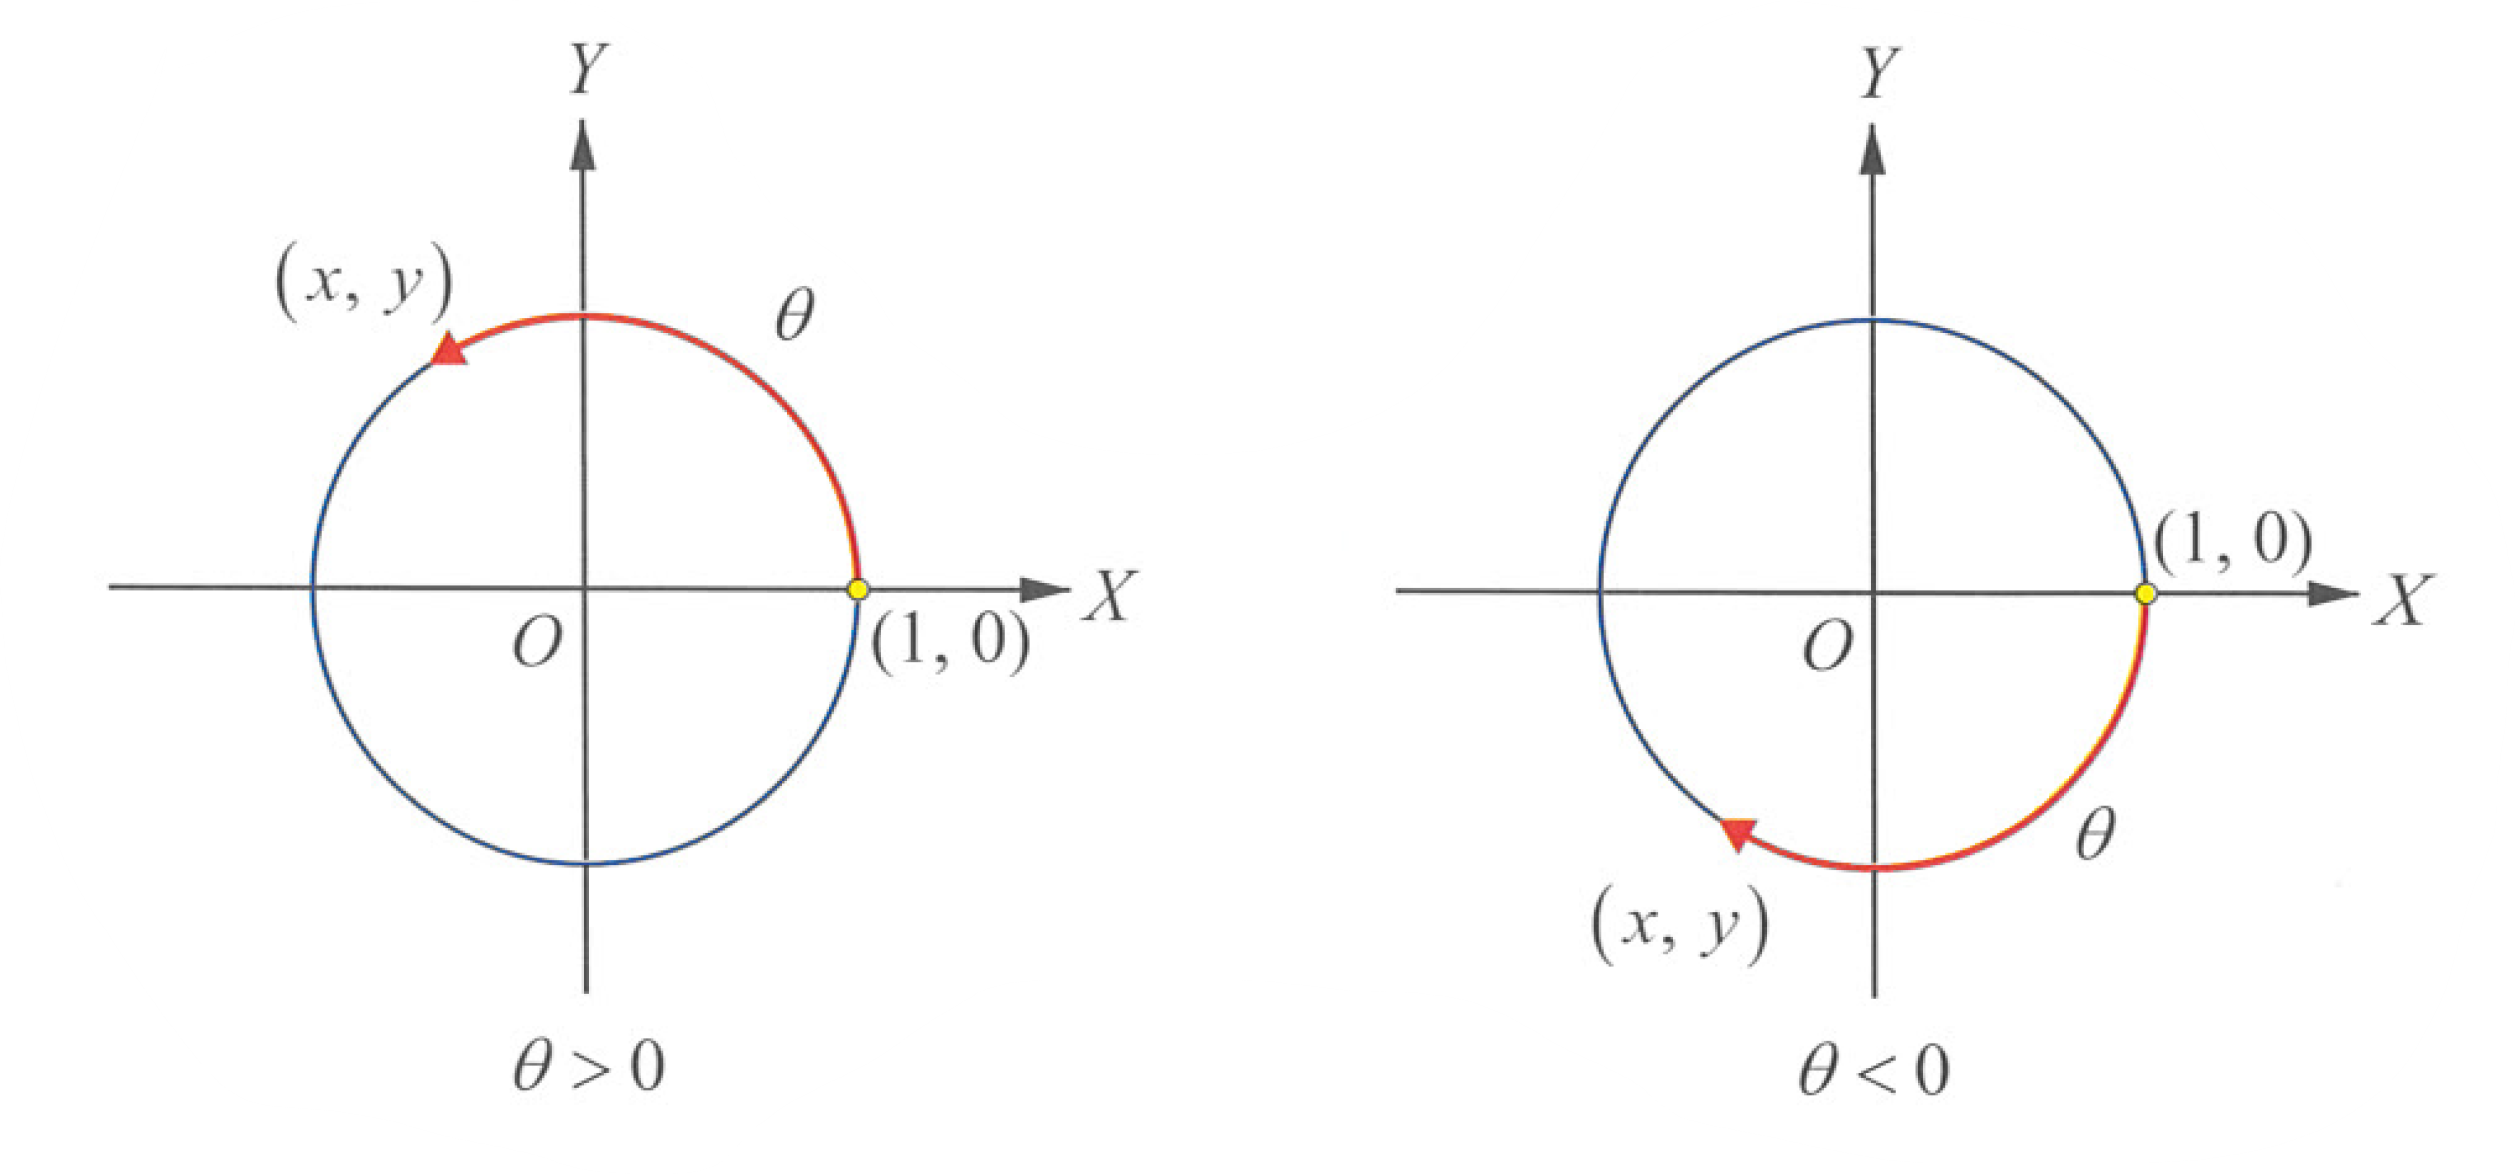
\includegraphics[scale=0.40]{1} 
	\caption{} 
	\label{Figure1} 
\end{figure}

รูปต่อไปนี้แสดงตำแหน่งของจุดปลายส่วนโค้งของวงกลมหนึ่งหน่วย เมื่อกำหนด $\theta$ ให้มีค่าต่าง ๆ กัน

\begin{figure}[H] 
	\centering 
	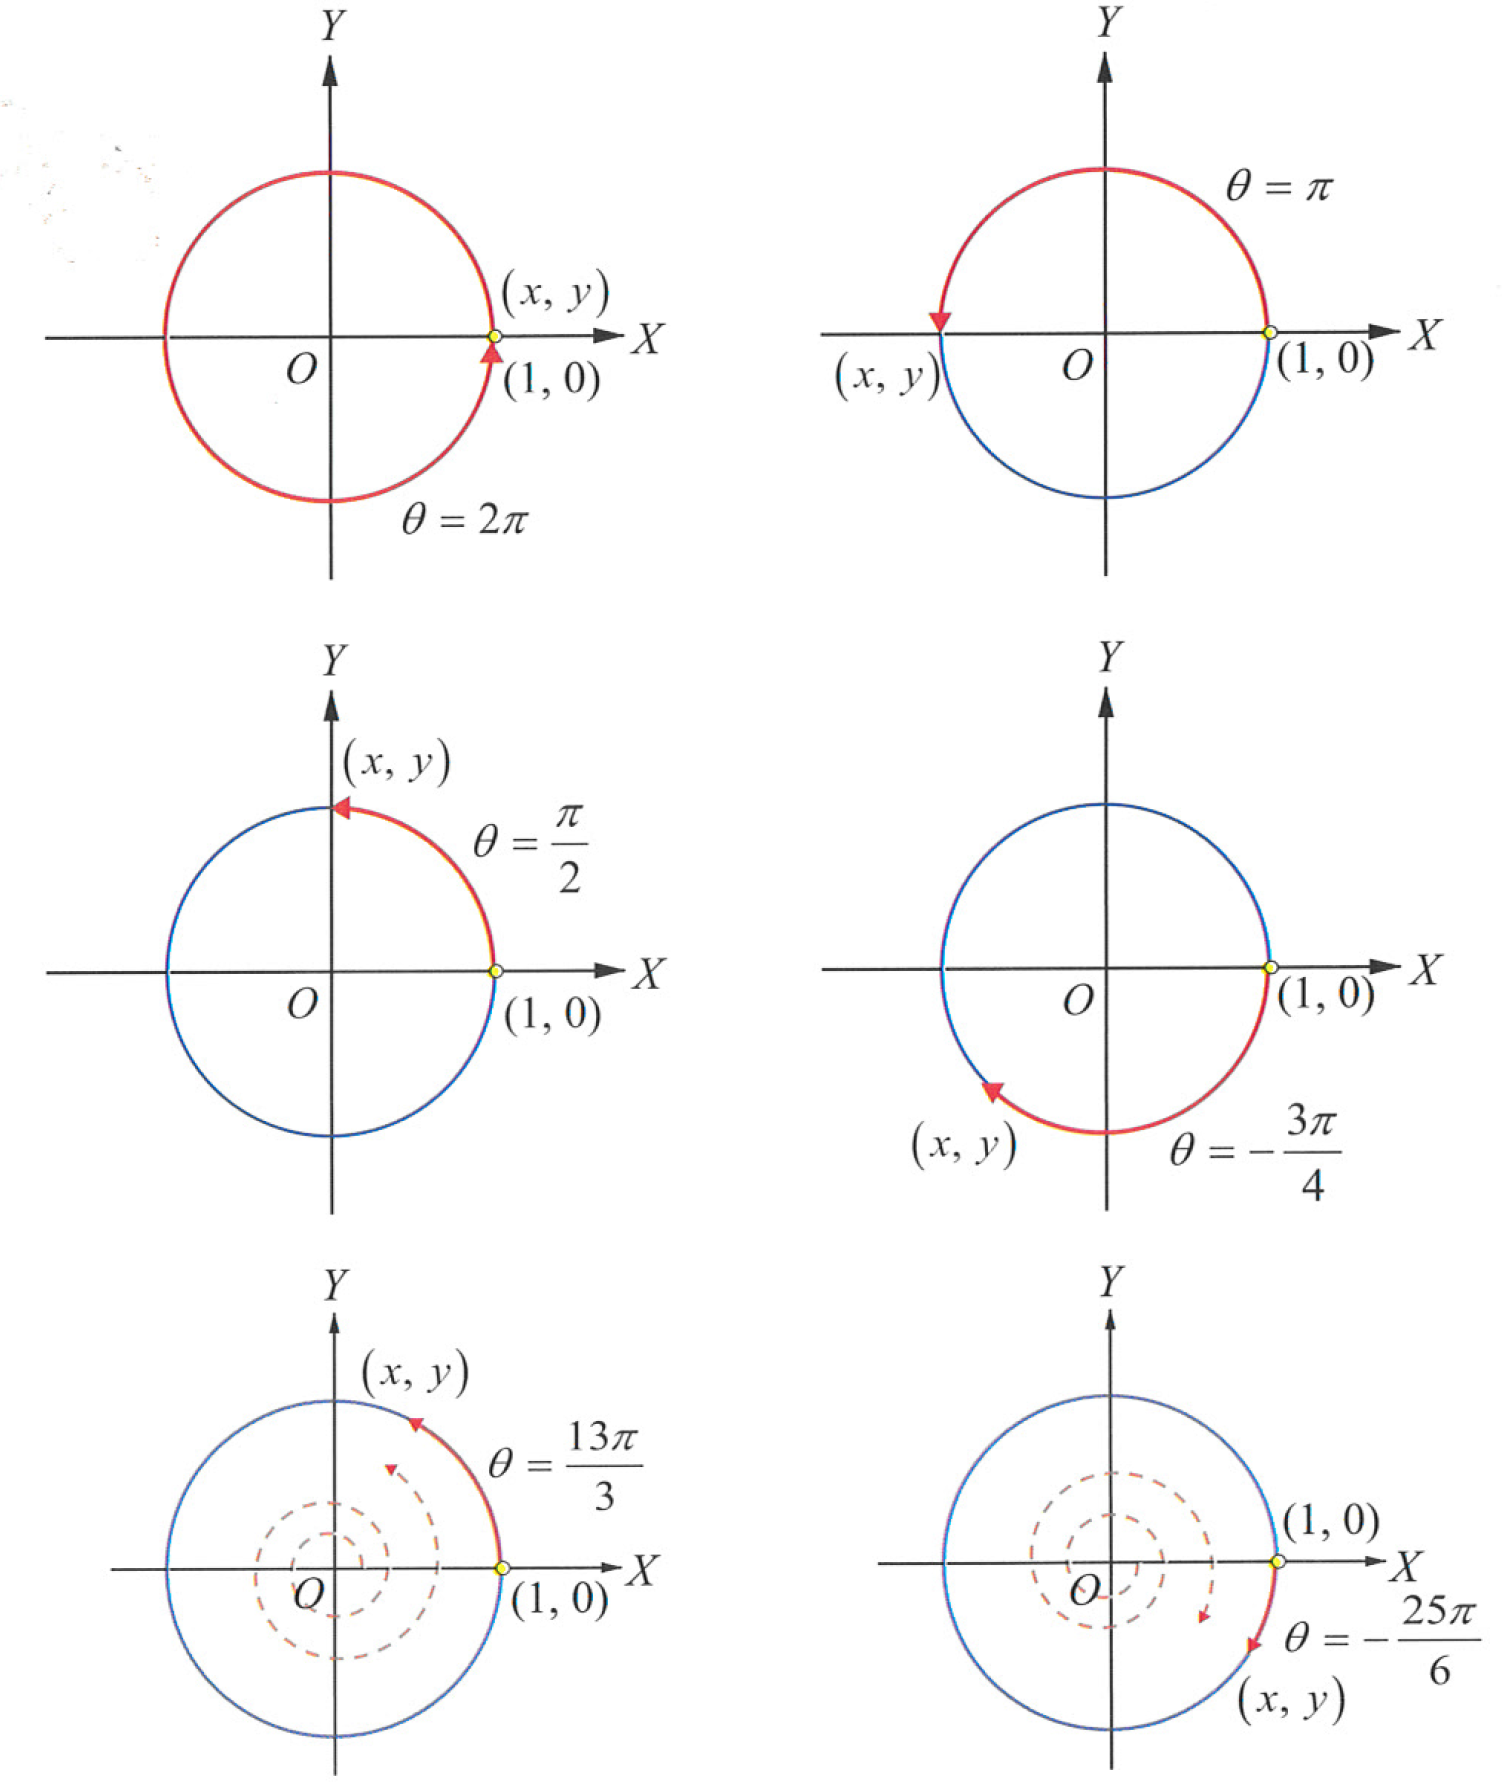
\includegraphics[scale=0.70]{2} 
	\caption{} 
	\label{Figure2} 
\end{figure}

จะเห็นว่า เมื่อกำหนดจำนวนจริง $\theta$ ให้ จะสามารถหาจุด $(x, y)$ ซึ่งเป็นจุดปลายส่วนโค้งที่ยาว $|\theta|$ หน่วย ในทิศทางการวัดที่กำหนดได้เพียงจุดเดียวเท่านั้น ถ้า $|\theta| > 2\pi$ แสดงว่าวัดส่วนโค้งเกิน $1$ รอบ เพราะเส้นรอบวงของวงกลมหนึ่งหน่วยยาว $2\pi$ หน่วย

\vspace{0.5em}
ดังนั้น จึงสามารถกำหนดฟังก์ชัน $f: \mathbb{R} \rightarrow \mathbb{R}$ และ $g: \mathbb{R} \rightarrow \mathbb{R}$ โดยที่สำหรับแต่ละจำนวนจริง $\theta$ ใด ๆ
$$f(\theta) = x$$
$$g(\theta) = y$$

เมื่อ $(x, y)$ เป็นจุดปลายส่วนโค้งของวงกลมหนึ่งหน่วยที่วัดจากจุด $(1,0)$ ยาว $|\theta|$ หน่วย ในทิศทางตามที่กล่าวข้างต้น

\vspace{0.5em}
เรียกฟังก์ชัน $g$ และ $f$ ดังกล่าวนี้ว่า \textbf{ฟังก์ชันไซน์ (sine function)} และ \textbf{ฟังก์ชันโคไซน์ (cosine function)} ตามลำดับ และจะเขียนแทน $g$ ด้วย $\sin$ และเขียนแทน $f$ ด้วย $\cos$ ดังนี้
$$y = \sin\theta \quad (\text{อ่านว่า วาย เท่ากับ ไซน์ทีตา})$$
$$x = \cos\theta \quad (\text{อ่านว่า เอกซ์ เท่ากับ คอสทีตา})$$

\vspace{0.5em}
วงกลมหนึ่งหน่วยซึ่งมีจุดศูนย์กลางอยู่ที่จุดกำเนิด เป็นกราฟของความสัมพันธ์
$$\left\{(x, y) \in \mathbb{R} \times \mathbb{R} \;\middle|\; x^2 + y^2 = 1\right\}$$

จะเห็นว่า $-1 \leq y \leq 1$ และ $-1 \leq x \leq 1$ ดังนั้น ค่าของฟังก์ชันไซน์และฟังก์ชันโคไซน์จะเป็นจำนวนจริงตั้งแต่ $-1$ ถึง $1$

\vspace{0.5em}
นั่นคือ เรนจ์ของฟังก์ชันไซน์และฟังก์ชันโคไซน์ คือเซตของจำนวนจริงตั้งแต่ $-1$ ถึง $1$ และโดเมนของฟังก์ชันทั้งสอง คือเซตของจำนวนจริง

\vspace{0.5em}
จากสมการ $x^2 + y^2 = 1, \; y = \sin\theta$ และ $x = \cos\theta$ จะได้ความสัมพันธ์ของ $\sin\theta$ และ $\cos\theta$ ดังนี้
$$(\cos\theta)^2 + (\sin\theta)^2 = 1 \quad \text{เมื่อ } \theta \text{ เป็นจำนวนจริง}$$
หรือ
$$\cos^2\theta + \sin^2\theta = 1 \quad \text{เมื่อ } \theta \text{ เป็นจำนวนจริง}$$

\vspace{1em}
\remark
\begin{itemize}
	\item $\cos^2\theta$  หมายถึง $(\cos\theta)(\cos\theta)$ 
	\item $\cos\theta^2$  หมายถึง $\cos$ ของจำนวนจริง $\theta^2$
\end{itemize}

\newpage
\subsection*{ค่าของฟังก์ชันไซน์และโคไซน์ของจำนวนจริงบางจำนวน}
ในหัวข้อนี้จะหาค่าของ $\sin \theta$ และ $\cos \theta$ สำหรับ $\theta$ บางค่าที่สามารถหาพิกัดของจุดปลายส่วนโค้ง ที่วัดจากจุด $(1,0)$ ยาว $|\theta|$ หน่วย ได้ด้วยวิธีง่าย ๆ

ถ้า $\theta=0$ จะได้ จุดปลายส่วนโค้งที่ยาว $0$ หน่วย คือ $(1,0)$ ดังรูป ดังนั้น $\sin 0=0$ และ $\cos 0=1$

\begin{figure}[H] 
	\centering 
	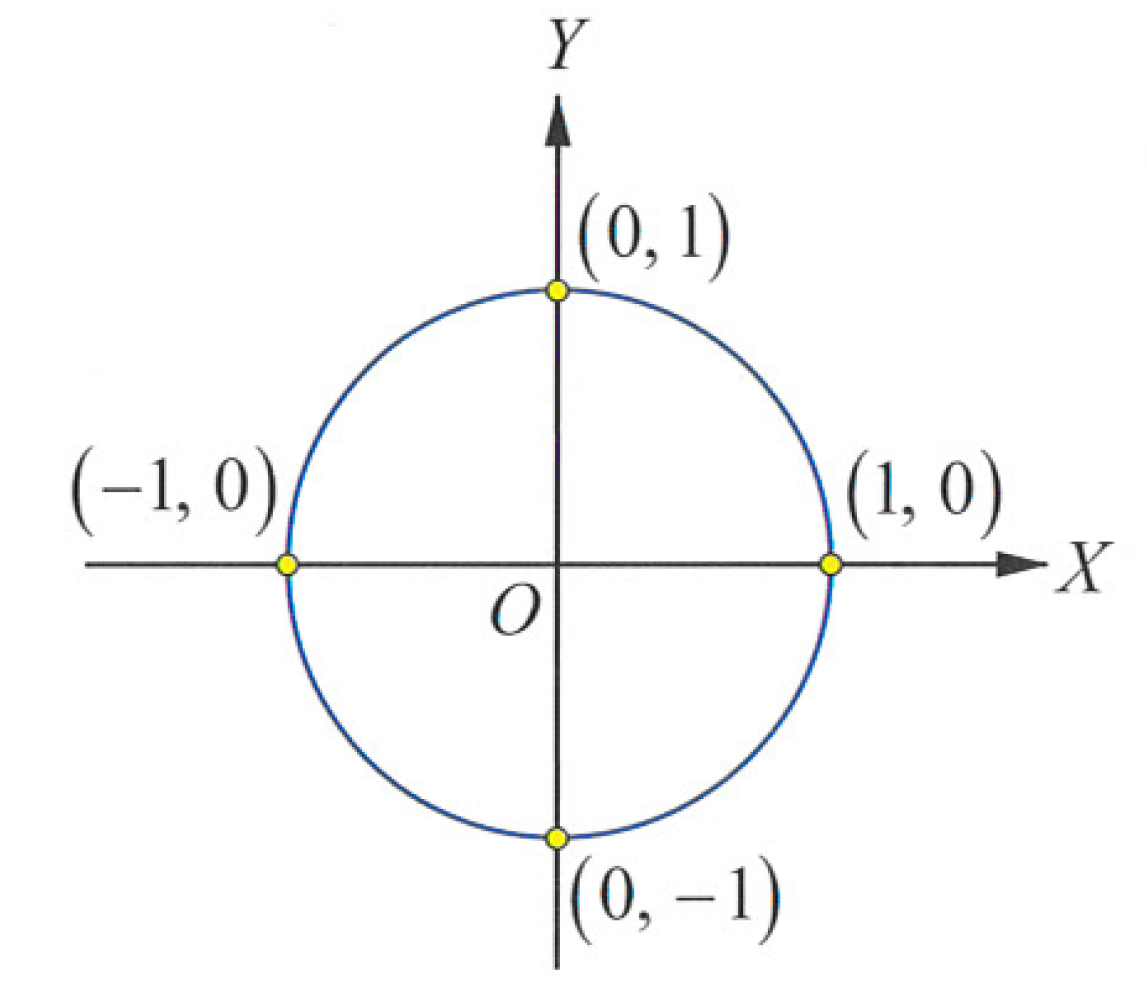
\includegraphics[scale=0.40]{3} 
	\caption{} 
	\label{Figure3} 
\end{figure}

เนื่องจากเส้นรอบวงของวงกลมหนึ่งหน่วยยาว $2\pi$ หน่วย และจุด $(1,0), \; (0,1), \; (-1,0)$ และ $(0,-1)$ เป็นจุดที่แบ่งเส้นรอบวงของวงกลมออกเป็นสี่ส่วนเท่า ๆ กัน โดยแต่ละส่วนยาว $\dfrac{\pi}{2}$ หน่วย ทำให้ได้ว่า

\vspace{1em}
$$\sin\dfrac{\pi}{2} = 1 \quad \text{และ} \quad \sin\left(-\dfrac{\pi}{2}\right) = -1$$
$$\sin\pi = 0 \quad \text{และ} \quad \sin(-\pi) = 0$$
$$\sin\dfrac{3\pi}{2} = -1 \quad \text{และ} \quad \sin\left(-\dfrac{3\pi}{2}\right) = 1$$
\vspace{0.5em}
$$\cos\dfrac{\pi}{2} = 0 \quad \text{และ} \quad \cos\left(-\dfrac{\pi}{2}\right) = 0$$
$$\cos\pi = -1 \quad \text{และ} \quad \cos(-\pi) = -1$$
$$\cos\dfrac{3\pi}{2} = 0 \quad \text{และ} \quad \cos\left(-\dfrac{3\pi}{2}\right) = 0$$
\vspace{1em}

จะเห็นว่า ค่าของ $\sin\theta$ และ $\cos\theta$ เมื่อ $\theta = \dfrac{n\pi}{2}$ โดยที่ $n$ เป็นจำนวนเต็ม หาได้จากพิกัดของจุดปลายส่วนโค้งที่ยาว $\left|\dfrac{n\pi}{2}\right|$ หน่วย โดยวัดในทิศทางที่สอดคล้องกับ $\theta$ ซึ่งจุดปลายนั้นจะเป็นจุดใดจุดหนึ่งในสี่จุดต่อไปนี้คือ $(1,0), \; (0,1), \; (-1,0)$ และ $(0,-1)$

\vspace{1em}
ต่อไปจะพิจารณาค่าของ $\sin\theta$ และ $\cos\theta$ เมื่อ $\theta$ เป็น $\dfrac{\pi}{4}, \; \dfrac{\pi}{6}$ และ $\dfrac{\pi}{3}$

\newpage
\subsection*{ค่าของ $\sin\dfrac{\pi}{4}$ และ $\cos\dfrac{\pi}{4}$}

\begin{figure}[H] 
	\centering 
	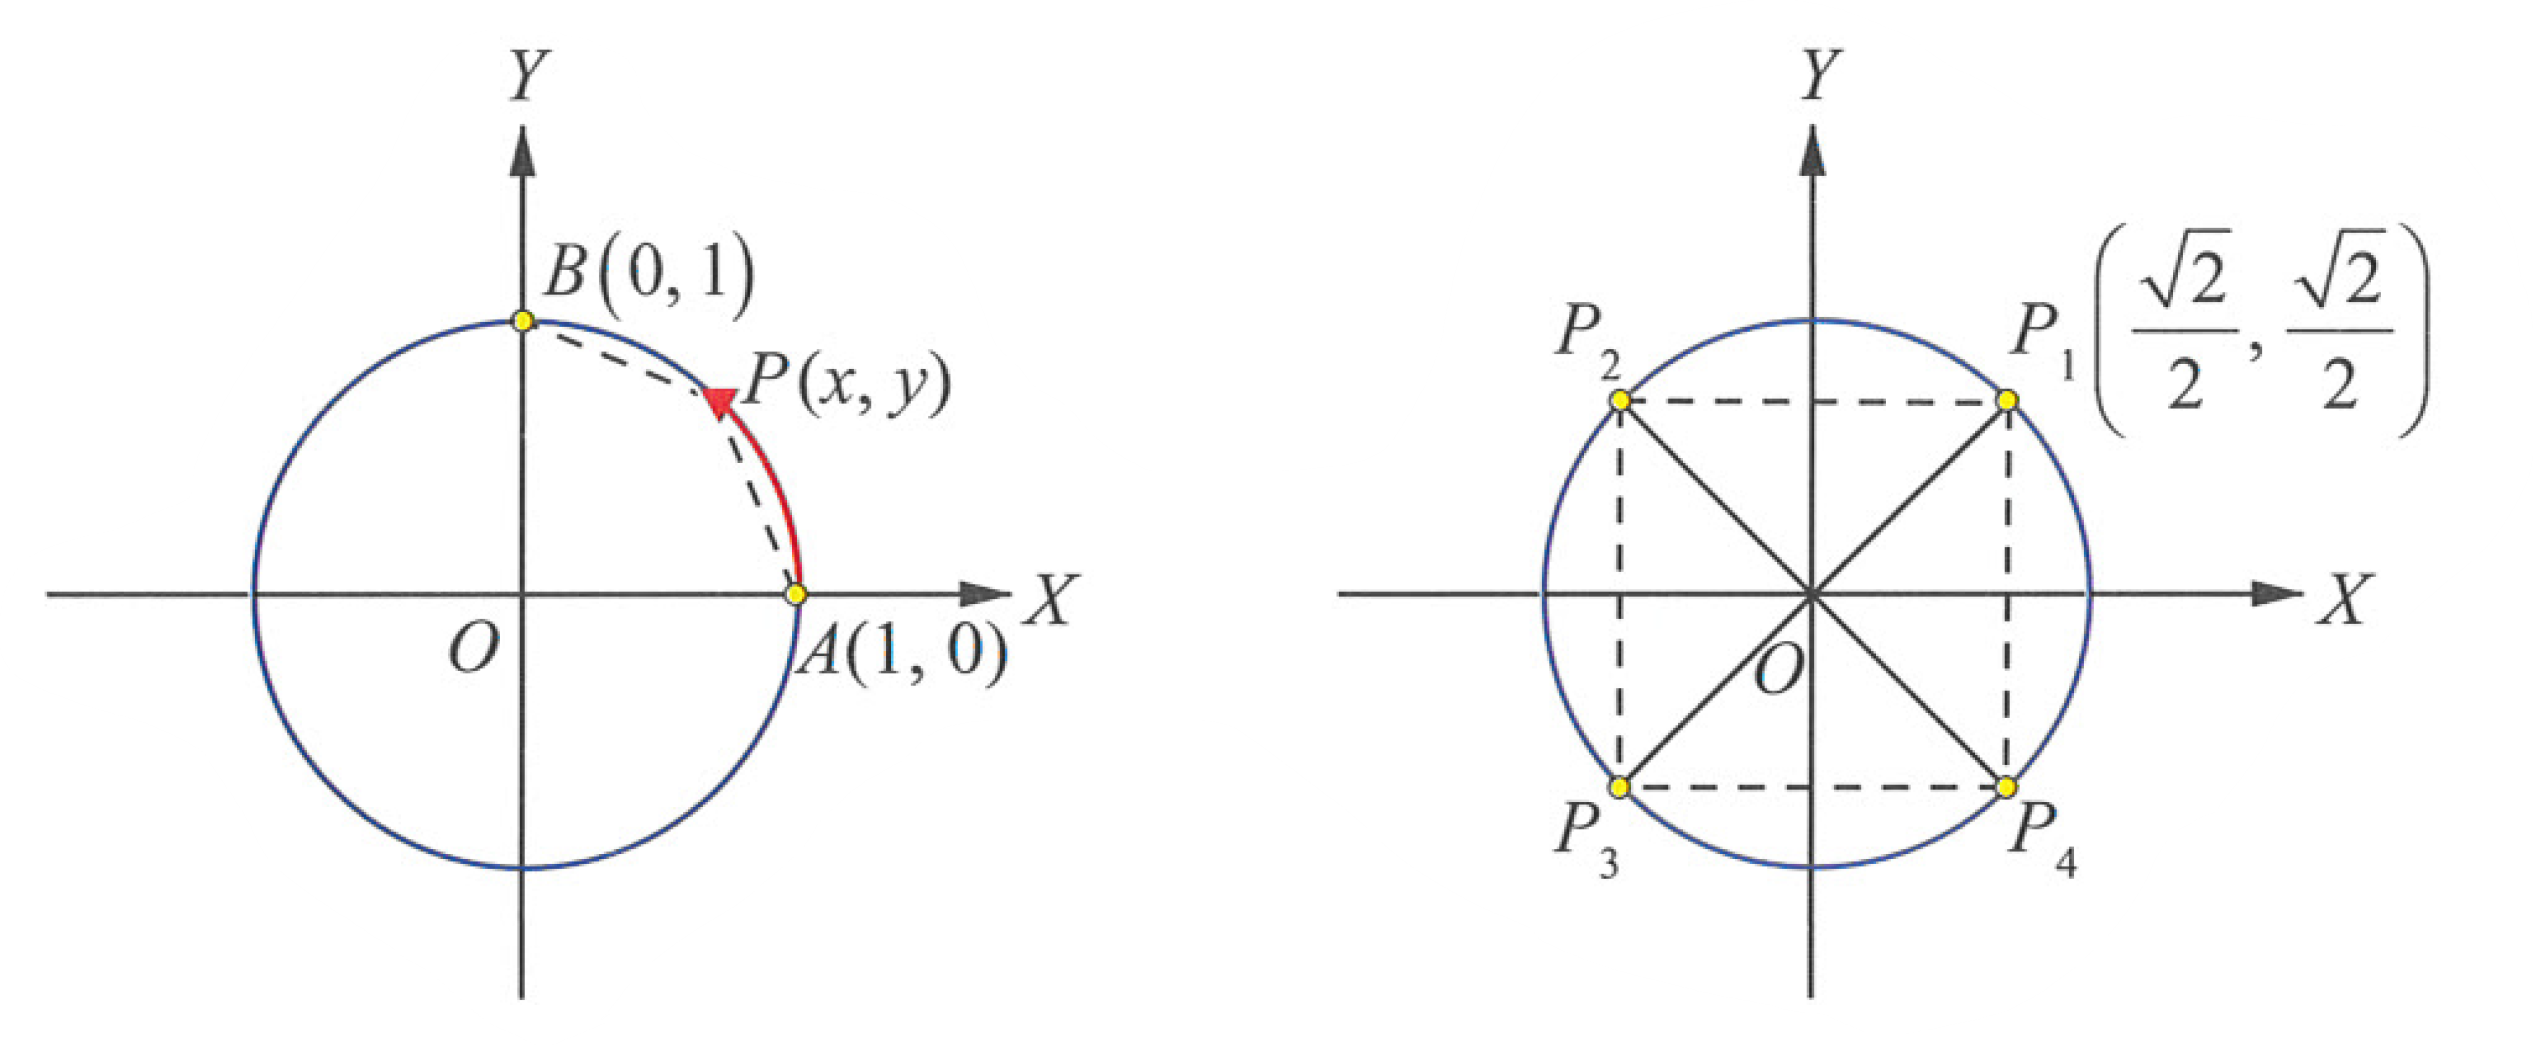
\includegraphics[scale=0.40]{4} 
	\caption{การหาพิกัดของจุดปลายส่วนโค้งที่ยาว $\dfrac{\pi}{4}$ หน่วย บนวงกลมหนึ่งหน่วย} 
	\label{Figure4} 
\end{figure}

\noindent ให้ $P(x, y)$ เป็นจุดกึ่งกลางของส่วนโค้ง $AB$ \\
เนื่องจากส่วนโค้ง $AB$ ยาว $\dfrac{\pi}{2}$ หน่วย 
\\
ดังนั้น ส่วนโค้ง $AP$ ยาวเท่ากับส่วนโค้ง $PB$ และยาว $\dfrac{\pi}{4}$ หน่วย ย่อมส่งผลให้คอร์ด $PB$ มีความยาวเท่ากับคอร์ด $PA$ นั่นคือ
$$PB = PA$$
$$\sqrt{x^2 + (y - 1)^2} = \sqrt{(x - 1)^2 + y^2}$$
$$x^2 + y^2 - 2y + 1 = x^2 - 2x + 1 + y^2$$

\vspace{0.5em}
\noindent เมื่อทอนพจน์ที่เหมือนกันทั้งสองข้างออก จะได้
$$x = y$$

\vspace{0.5em}
\noindent แต่เนื่องจาก $P(x, y)$ เป็นจุดที่อยู่บนวงกลมหนึ่งหน่วย ซึ่งสอดคล้องกับสมบัติ 
$$x^2 + y^2 = 1$$
เมื่อแทนค่า $y = x$ ลงในสมการข้างต้น จะได้
$$2x^2 = 1$$
$$x^2 = \dfrac{1}{2}$$

\vspace{0.5em}
\noindent ถอดรากที่สองเพื่อหาค่าตัวแปร จะได้
$$x = \dfrac{1}{\sqrt{2}} \quad \text{หรือ} \quad x = -\dfrac{1}{\sqrt{2}}$$

\vspace{0.8em}
\noindent เนื่องจากจุด $P(x, y)$ เป็นจุดกึ่งกลางส่วนโค้งในจตุภาคที่ 1 (Quadrant I) ย่อมส่งผลให้ทั้งพิกัด $x$ และ $y$ ต้องเป็นจำนวนจริงบวกเท่านั้น 
\\
ดังนั้น จึงเลือกใช้เฉพาะค่าบวก ทำให้ได้ว่า
$$x = y = \dfrac{1}{\sqrt{2}} = \dfrac{\sqrt{2}}{2}$$

\vspace{0.8em}
\noindent สรุปได้ว่า จุดปลายส่วนโค้งที่ยาว $\dfrac{\pi}{4}$ หน่วย โดยวัดในทิศทางทวนเข็มนาฬิกา คือ จุด $\left(\dfrac{\sqrt{2}}{2}, \; \dfrac{\sqrt{2}}{2}\right)$ นั่นคือ
$$\sin\dfrac{\pi}{4} = \dfrac{\sqrt{2}}{2} \quad \text{และ} \quad \cos\dfrac{\pi}{4} = \dfrac{\sqrt{2}}{2}$$

\newpage
\subsection*{ค่าของ $\sin\dfrac{\pi}{6}$ และ $\cos\dfrac{\pi}{6}$}

\begin{figure}[H] 
	\centering 
	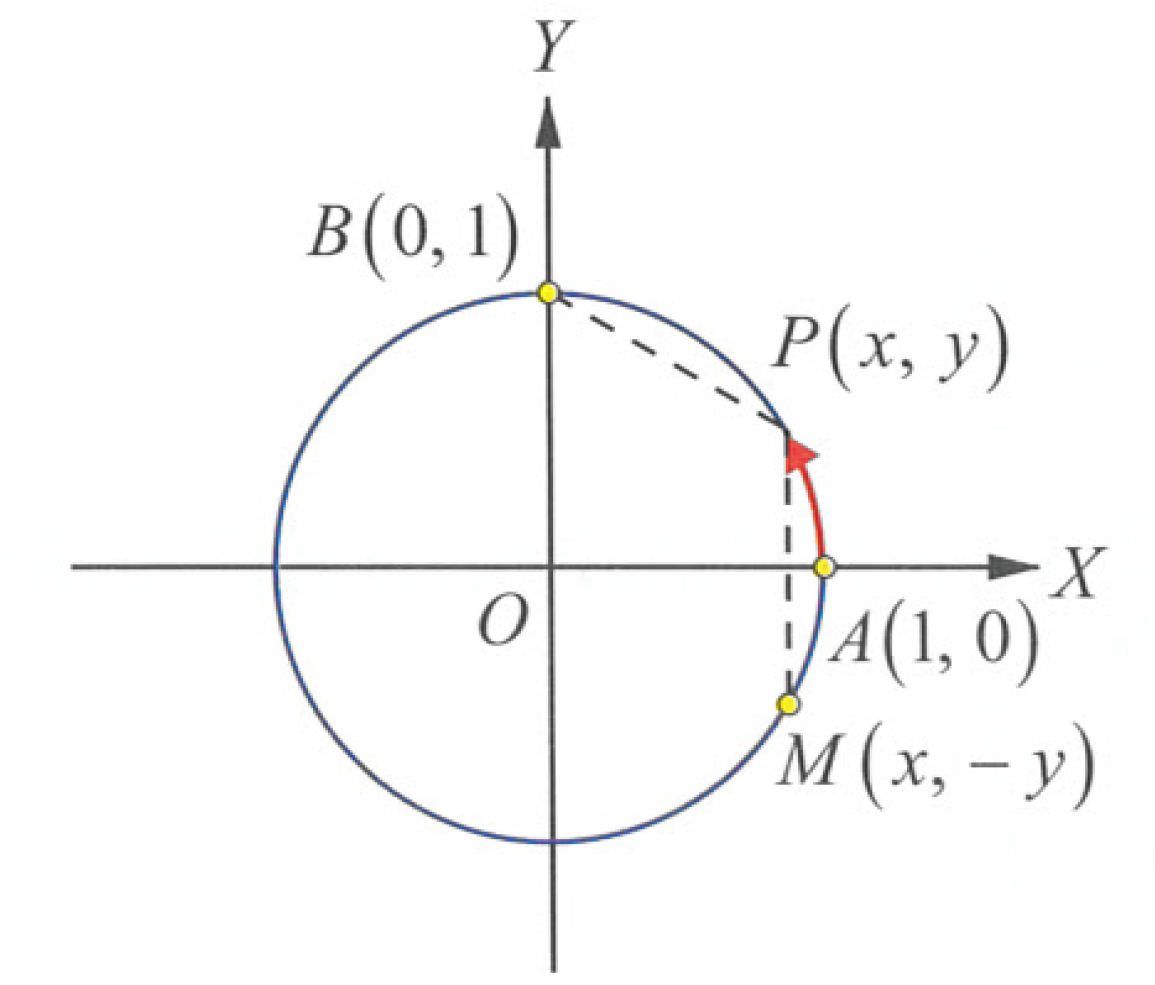
\includegraphics[scale=0.40]{5} 
	\caption{การหาพิกัดของจุดปลายส่วนโค้งที่ยาว $\dfrac{\pi}{6}$ หน่วย บนวงกลมหนึ่งหน่วย} 
	\label{Figure5} 
\end{figure}

\noindent ให้ $P(x, y)$ เป็นจุดบนส่วนโค้ง $AB$ ที่ทำให้ส่วนโค้ง $AP$ ยาว $\dfrac{\pi}{6}$ หน่วย 
\\
เนื่องจากส่วนโค้ง $AB$ ยาว $\dfrac{\pi}{2}$ หน่วย ดังนั้น ส่วนโค้ง $PB$ ยาว $\dfrac{\pi}{2} - \dfrac{\pi}{6} = \dfrac{\pi}{3}$ หน่วย 

\vspace{0.5em}
\noindent ให้จุด $M$ เป็นภาพสะท้อนของจุด $P$ โดยมีแกน $X$ เป็นเส้นสะท้อน จะได้ส่วนโค้ง $AM$ ยาวเท่ากับส่วนโค้ง $AP$ ซึ่งยาว $\dfrac{\pi}{6}$ หน่วย และจุด $M$ มีพิกัดเป็น $(x, -y)$ 
\\
ดังนั้น ส่วนโค้ง $PM$ ยาว $\dfrac{\pi}{6} + \dfrac{\pi}{6} = \dfrac{\pi}{3}$ หน่วย ย่อมส่งผลให้คอร์ด $PM$ มีความยาวเท่ากับคอร์ด $PB$ นั่นคือ
$$PM = PB$$
$$\sqrt{(x - x)^2 + (y - (-y))^2} = \sqrt{(x - 0)^2 + (y - 1)^2}$$
$$4y^2 = x^2 + y^2 - 2y + 1$$

\vspace{0.3em}
\noindent เนื่องจากจุด $P(x, y)$ อยู่บนวงกลมหนึ่งหน่วย ซึ่งสอดคล้องกับสมบัติ $x^2 + y^2 = 1$ เมื่อแทนค่าลงในสมการข้างต้น จะได้
$$4y^2 + 2y - 2 = 0$$
$$2y^2 + y - 1 = 0$$
$$(2y - 1)(y + 1) = 0$$

\vspace{0.3em}
\noindent เมื่อแก้สมการกำลังสอง จะได้
$$y = \dfrac{1}{2} \quad \text{หรือ} \quad y = -1$$

\vspace{0.5em}
\noindent เนื่องจากจุด $P(x, y)$ เป็นจุดในจตุภาคที่ 1 (Quadrant I) ย่อมส่งผลให้ทั้งพิกัด $x$ และ $y$ ต้องเป็นจำนวนจริงบวกเท่านั้น 
\\
ดังนั้น จึงเลือกใช้เฉพาะค่าบวก ทำให้ได้ว่า
$$y = \dfrac{1}{2}$$

\vspace{0.5em}
\noindent และจากสมบัติ $x^2 + y^2 = 1$ เมื่อแทนค่า $y$ ลงไปจะได้ $x^2 = 1 - \left(\dfrac{1}{2}\right)^2 = \dfrac{3}{4}$ ถอดรากฝั่งค่าบวกจะได้
$$x = \dfrac{\sqrt{3}}{2}$$

\vspace{0.5em}
\noindent สรุปได้ว่า จุดปลายส่วนโค้งที่ยาว $\dfrac{\pi}{6}$ หน่วย โดยวัดในทิศทางทวนเข็มนาฬิกา คือ จุด $\left(\dfrac{\sqrt{3}}{2}, \; \dfrac{1}{2}\right)$ นั่นคือ
$$\sin\dfrac{\pi}{6} = \dfrac{1}{2} \quad \text{และ} \quad \cos\dfrac{\pi}{6} = \dfrac{\sqrt{3}}{2}$$

\newpage
\subsection*{ค่าของ $\sin\dfrac{\pi}{3}$ และ $\cos\dfrac{\pi}{3}$}

\begin{figure}[H] 
	\centering 
	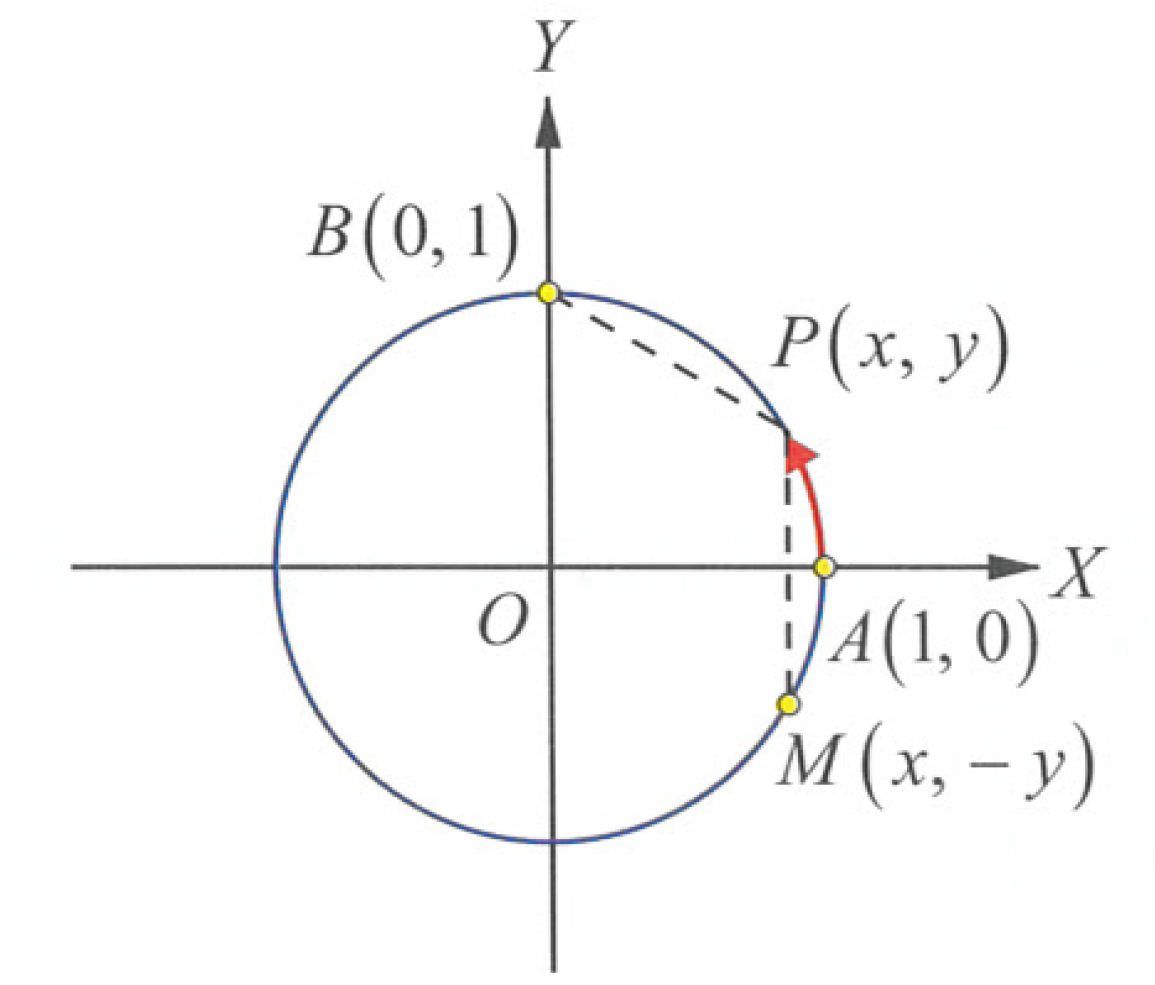
\includegraphics[scale=0.40]{5} 
	\caption{การหาพิกัดของจุดปลายส่วนโค้งที่ยาว $\dfrac{\pi}{3}$ หน่วย บนวงกลมหนึ่งหน่วย} 
	\label{Figure5} 
\end{figure}

\noindent สำหรับการหาค่าของ $\sin\dfrac{\pi}{3}$ และ $\cos\dfrac{\pi}{3}$ สามารถพิจารณาได้ในทำนองเดียวกัน โดยให้ $Q(x, y)$ เป็นจุดปลายส่วนโค้งที่ยาว $\dfrac{\pi}{3}$ หน่วยในจตุภาคที่ 1 

\vspace{0.5em}
\noindent เนื่องจากส่วนโค้ง $AQ$ ยาว $\dfrac{\pi}{3}$ หน่วย ทำให้ส่วนโค้งที่เหลือ $QB$ ยาว $\dfrac{\pi}{2} - \dfrac{\pi}{3} = \dfrac{\pi}{6}$ หน่วย 
\\
เมื่อพิจารณาภาพสะท้อนข้ามเส้นตรง $y = x$ หรืออาศัยสมมาตรของส่วนโค้งเทียบกับหัวข้อ $\dfrac{\pi}{6}$ ที่ผ่านกระบวนการพิสูจน์ข้างต้น จะได้ว่าพิกัดของจุด $Q$ จะสลับตแหน่งกับพิกัดของจุด $P$ บนส่วนโค้งที่ยาว $\dfrac{\pi}{6}$ หน่วย นั่นคือ
$$x = \dfrac{1}{2} \quad \text{และ} \quad y = \dfrac{\sqrt{3}}{2}$$

\vspace{0.5em}
\noindent สรุปได้ว่า จุดปลายส่วนโค้งที่ยาว $\dfrac{\pi}{3}$ หน่วย โดยวัดในทิศทางทวนเข็มนาฬิกา คือ จุด $\left(\dfrac{1}{2}, \; \dfrac{\sqrt{3}}{2}\right)$ นั่นคือ
$$\sin\dfrac{\pi}{3} = \dfrac{\sqrt{3}}{2} \quad \text{และ} \quad \cos\dfrac{\pi}{3} = \dfrac{1}{2}$$

\newpage
\subsection*{ค่าของฟังก์ชันไซน์และโคไซน์ของจำนวนจริงใด ๆ}

พิจารณาจำนวนจริง $\theta > 0$ และให้ $(x, y)$ เป็นจุดปลายส่วนโค้งของวงกลมหนึ่งหน่วยที่วัดจากจุด $(1,0)$ ไปในทิศทางทวนเข็มนาฬิกาเป็นระยะทาง $\theta$ หน่วย (เนื่องจาก $\theta > 0$ จึงได้ $|\theta| = \theta$) 

\vspace{0.5em}
เมื่อสะท้อนจุด $(x, y)$ โดยมีแกน $X$ เป็นเส้นสะท้อน จะได้จุด $(x, -y)$ เป็นภาพสะท้อน ย่อมส่งผลให้จุด $(x, -y)$ เป็นจุดปลายส่วนโค้งของวงกลมดังกล่าวที่วัดจากจุด $(1,0)$ ไปในทิศทางตามเข็มนาฬิกาเป็นระยะทาง $\theta$ หน่วย ดังรูป หรือกล่าวตามข้อตกลงเรื่องการวัดส่วนโค้งได้ว่า $(x, -y)$ เป็นจุดปลายของส่วนโค้งที่เกิดจากจำนวนจริง $-\theta$

\vspace{1em}

\begin{figure}[H] 
	\centering 
	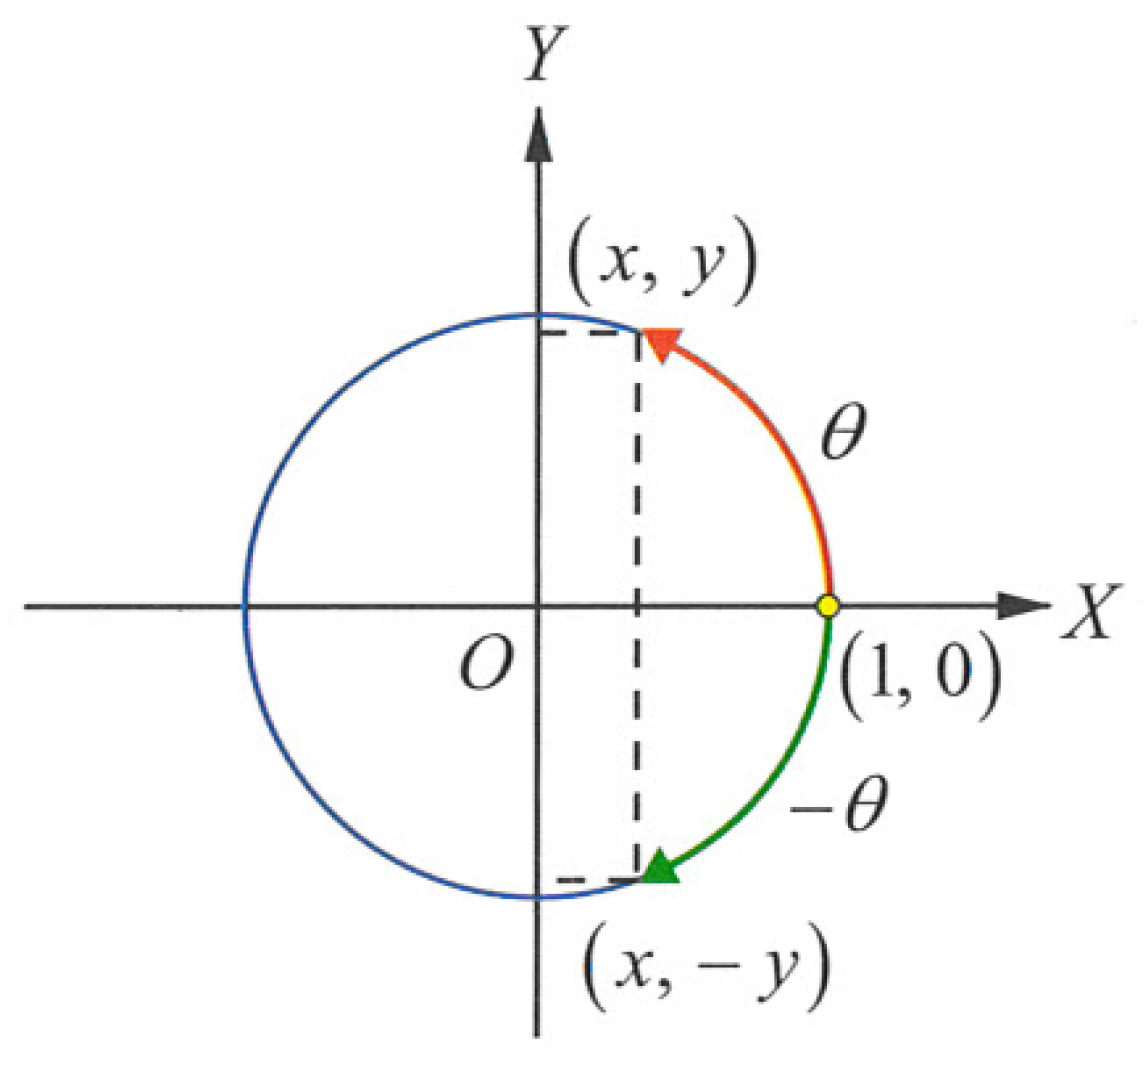
\includegraphics[scale=0.40]{7} 
	\caption{พิกัดของจุดปลายส่วนโค้งบนวงกลมหนึ่งหน่วยสำหรับจำนวนจริง $\theta$ และ $-\theta$} 
	\label{Figure7} 
\end{figure}

\vspace{1em}
\noindent จากพิกัดของจุด $(x, y)$ และจุดปลายภาพสะท้อน $(x, -y)$ จะได้ว่า
$$\cos\theta = x \quad \text{และ} \quad \sin\theta = y$$
และ
$$\cos(-\theta) = x \quad \text{และ} \quad \sin(-\theta) = -y$$

\vspace{0.5em}
\noindent เมื่อเปรียบเทียบพิกัดตัวแปรทั้งสองระบบ จึงสรุปเป็นความสัมพันธ์ได้ดังนี้
$$\sin(-\theta) = -\sin\theta$$
$$\cos(-\theta) = \cos\theta$$

\vspace{1em}
\noindent นั่นคือ ถ้าสามารถหาค่าของฟังก์ชันไซน์และโคไซน์ของจำนวนจริงบวกใด ๆ ได้ ก็จะสามารถหาค่าของฟังก์ชันไซน์และโคไซน์ของจำนวนจริงลบที่เป็นตัวผกผันการบวกของจำนวนจริงบวกนั้น ๆ ได้ด้วย

\begin{examplebox}
	จงหาค่าของ $\sin\left(-\dfrac{\pi}{6}\right)$ และ $\cos\left(-\dfrac{\pi}{6}\right)$
\end{examplebox}
\solution
\vspace{0.5em}
\noindent จากสมบัติมุมผกผันและค่ามาตรฐาน เนื่องจาก $\sin\dfrac{\pi}{6} = \dfrac{1}{2}$ และ $\cos\dfrac{\pi}{6} = \dfrac{\sqrt{3}}{2}$
\\
จะได้
$$\sin\left(-\dfrac{\pi}{6}\right) = -\sin\dfrac{\pi}{6} = -\dfrac{1}{2}$$
และ
$$\cos\left(-\dfrac{\pi}{6}\right) = \cos\dfrac{\pi}{6} = \dfrac{\sqrt{3}}{2}$$

\vspace{1.5em}
\noindent เนื่องจากเส้นรอบวงของวงกลมหนึ่งหน่วยมีความยาว $2\pi$ หน่วย ดังนั้น จุดปลายของส่วนโค้งบนเส้นรอบวงของวงกลมหนึ่งหน่วยที่ยาว $2n\pi + \theta$ หน่วย จะเป็นจุดเดียวกับจุดปลายของส่วนโค้งที่ยาว $\theta$ หน่วย 

\vspace{0.5em}
\noindent โดยที่เมื่อ $n$ เป็นจำนวนเต็มบวก จะเป็นการวัดระยะในทิศทางทวนเข็มนาฬิกาซ้ำจำนวน $n$ รอบ แต่ถ้า $n$ เป็นจำนวนเต็มลบ จะเป็นการวัดระยะในทิศทางตามเข็มนาฬิกาซ้ำจำนวน $n$ รอบ จึงสรุปความสัมพันธ์ในกรณีทั่วไปได้ดังนี้

\vspace{1em}
\noindent เมื่อ $n$ เป็นจำนวนเต็มใด ๆ จะได้ว่า
$$\sin(2n\pi + \theta) = \sin\theta$$
$$\cos(2n\pi + \theta) = \cos\theta$$

\vspace{1em}
\noindent จากสมบัติข้างต้นนี้ จะเห็นว่าถ้าเราสามารถหาค่าของฟังก์ชันไซน์และโคไซน์ของจำนวนจริงที่มีค่าตั้งแต่ $0$ ถึง $2\pi$ ได้แล้ว ย่อมสามารถหาค่าของฟังก์ชันไซน์และโคไซน์ของจำนวนจริงทุกจำนวนบนระบบทางคณิตศาสตร์ได้เสมอ

\begin{examplebox}
	จงหาค่าของ $\sin\left(\dfrac{25\pi}{4}\right)$ และ $\cos\left(-\dfrac{11\pi}{3}\right)$
\end{examplebox}
\solution
\vspace{6cm}

\noindent จากที่ทราบว่า เมื่อหาค่าของฟังก์ชันไซน์และโคไซน์ของจำนวนจริงตั้งแต่ $0$ ถึง $2\pi$ ได้ ก็จะหาค่าของฟังก์ชันไซน์และโคไซน์ของจำนวนจริงใด ๆ ได้ 
\\
แต่เนื่องจากวงกลมหนึ่งหน่วยมีแกน $X$ และแกน $Y$ เป็นแกนสมมาตร การหาค่าของฟังก์ชันไซน์และโคไซน์ของจำนวนจริงตั้งแต่ $0$ ถึง $2\pi$ จึงหาได้จากค่าของฟังก์ชันไซน์และโคไซน์ของจำนวนจริงตั้งแต่ $0$ ถึง $\dfrac{\pi}{2}$ ดังแสดงได้ดังนี้


\subsection*{1. เมื่อจุดปลายส่วนโค้งที่ยาว $\theta$ หน่วย อยู่ในจตุภาคที่ $2$ $\left(\dfrac{\pi}{2} < \theta < \pi\right)$}

\begin{figure}[H] 
	\centering 
	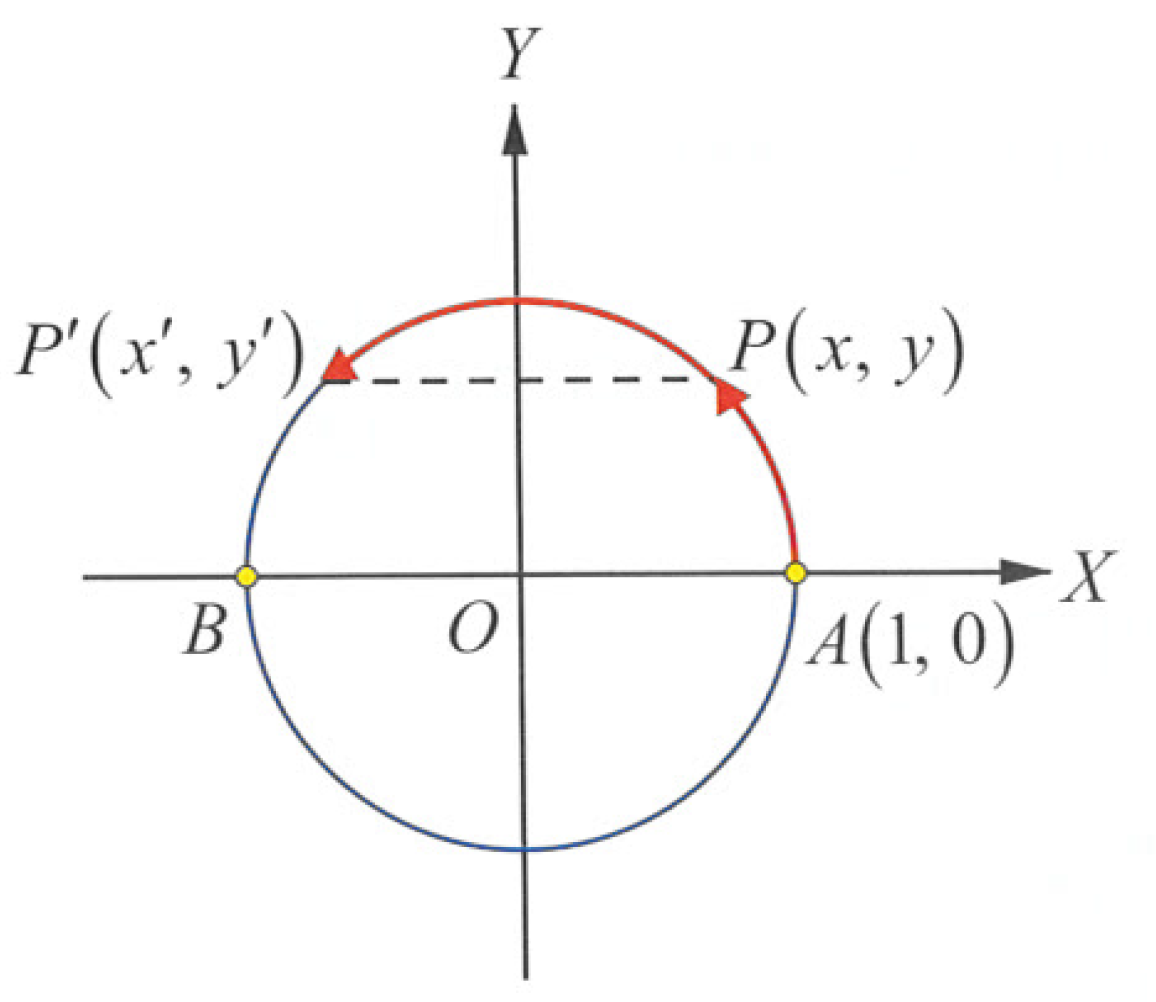
\includegraphics[scale=0.40]{8} 
	\caption{} 
	\label{Figure8} 
\end{figure}

\noindent ให้ $P^{\prime}(x^{\prime}, y^{\prime})$ เป็นจุดปลายส่วนโค้งที่ยาว $\theta$ หน่วย 
\\
ดังนั้น $y^{\prime} = \sin\theta$ และ $x^{\prime} = \cos\theta$
\\
ให้ $\alpha = \pi - \theta$ จะได้ว่า $0 < \alpha < \dfrac{\pi}{2}$

\vspace{0.5em}
\noindent เนื่องจากส่วนโค้งของครึ่งวงกลมยาว $\pi$ หน่วย ดังนั้น ส่วนโค้งจากจุดปลายไปยังแกน $X$ ทางซ้ายจึงยาว $\alpha$ หน่วย 
\\
เมื่อให้จุด $P(x, y)$ เป็นภาพสะท้อนของจุด $P^{\prime}(x^{\prime}, y^{\prime})$ โดยมีแกน $Y$ เป็นเส้นสะท้อน จะได้ว่าส่วนโค้ง $AP$ ในจตุภาคที่ 1 ยาว $\alpha$ หน่วย และมีความสัมพันธ์ของพิกัดเป็น $y^{\prime} = y$ และ $x^{\prime} = -x$

\vspace{0.5em}
\noindent เนื่องจาก $P(x, y)$ เป็นจุดปลายส่วนโค้งที่ยาว $\alpha$ หน่วยในจตุภาคที่ 1 
\\
ดังนั้น
$$y = \sin\alpha \quad \text{และ} \quad x = \cos\alpha$$

\vspace{0.3em}
\noindent เมื่อจับคู่เทียบความสัมพันธ์กับจุดสะท้อน จะได้ว่า
$$y^{\prime} = y \implies \sin\theta = \sin\left(\dfrac{\pi}{2} - \text{หรือการจัดรูปปกติ}\right)$$
$$\sin\theta = \sin(\pi - \alpha) = \sin\alpha$$
\\[0.3em]
และ
$$x^{\prime} = -x \implies \cos\theta = \cos(\pi - \alpha) = -\cos\alpha$$

\vspace{1em}
\noindent สรุปความสัมพันธ์เชิงเรขาคณิตสำหรับจตุภาคที่ 2 ได้ดังนี้
$$\sin(\pi - \alpha) = \sin\alpha \quad \text{เมื่อ} \quad 0 < \alpha < \dfrac{\pi}{2}$$
$$\cos(\pi - \alpha) = -\cos\alpha \quad \text{เมื่อ} \quad 0 < \alpha < \dfrac{\pi}{2}$$

\begin{examplebox}
	กำหนดให้ $\sin\left(\dfrac{\pi}{12}\right) \approx \dfrac{13}{50}$ จงหาค่าประมาณของ
	\begin{enumerate}
		\item $\sin\left(\dfrac{11\pi}{12}\right)$
		\item $\cos\left(\dfrac{11\pi}{12}\right)$
	\end{enumerate}
\end{examplebox}
\solution

\newpage

\subsection*{2. เมื่อจุดปลายส่วนโค้งที่ยาว $\theta$ หน่วย อยู่ในจตุภาคที่ $3$ $\left(\pi < \theta < \dfrac{3\pi}{2}\right)$}

\begin{figure}[H] 
	\centering 
	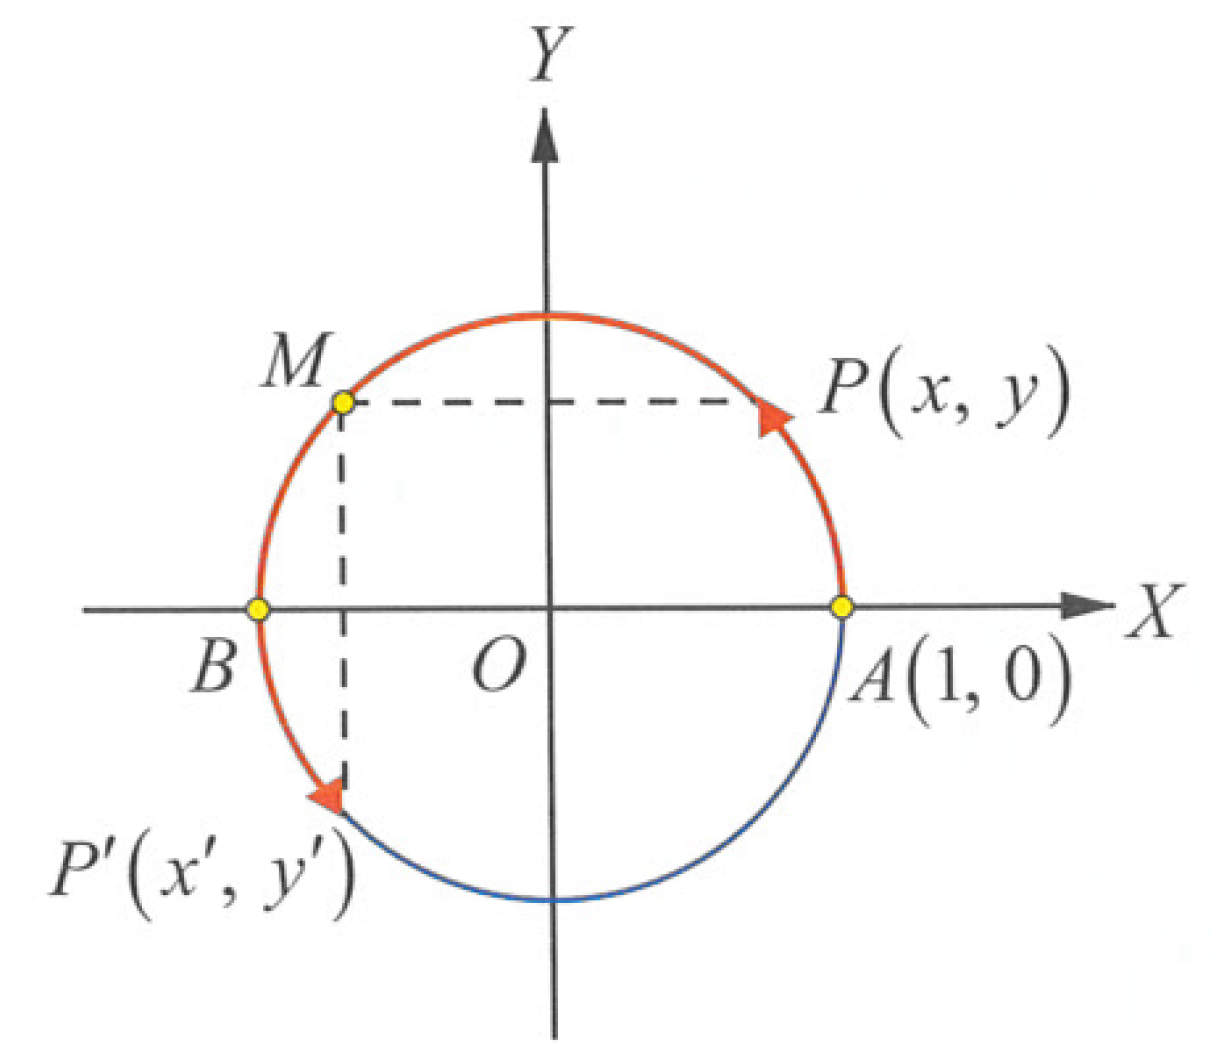
\includegraphics[scale=0.40]{9} 
	\caption{} 
	\label{Figure9} 
\end{figure}

\noindent ให้ $P^{\prime}(x^{\prime}, y^{\prime})$ เป็นจุดปลายส่วนโค้งที่ยาว $\theta$ หน่วย 
\\
ดังนั้น $y^{\prime} = \sin\theta$ และ $x^{\prime} = \cos\theta$
\\
ให้ $\alpha = \theta - \pi$ จะได้ว่า $0 < \alpha < \dfrac{\pi}{2}$

\vspace{0.5em}
\noindent เนื่องจากส่วนโค้งของครึ่งวงกลมยาว $\pi$ หน่วย ดังนั้น ส่วนโค้งจากจุดปลายแกน $X$ ทางซ้ายมายังจุด $P^{\prime}$ ย่อมยาว $\alpha$ หน่วย 
\\
เมื่อกำหนดให้จุด $M$ เป็นภาพสะท้อนของจุด $P^{\prime}(x^{\prime}, y^{\prime})$ โดยมีแกน $X$ เป็นเส้นสะท้อน และจุด $P(x, y)$ เป็นภาพสะท้อนของจุด $M$ โดยมีแกน $Y$ เป็นเส้นสะท้อน 
\\
จะได้ว่าส่วนโค้ง $AP$ ในจตุภาคที่ 1 ยาว $\alpha$ หน่วย และมีความสัมพันธ์ของพิกัดสะท้อนเป็น $y^{\prime} = -y$ และ $x^{\prime} = -x$

\vspace{0.5em}
\noindent เนื่องจากจุด $P(x, y)$ เป็นจุดปลายส่วนโค้งที่ยาว $\alpha$ หน่วยในจตุภาคที่ 1
\\
ดังนั้น 
$$y = \sin\alpha \quad \text{และ} \quad x = \cos\alpha$$

\vspace{0.3em}
\noindent เมื่อพิจารณาความสัมพันธ์ร่วมกับพิกัดจุดสะท้อนข้ามสองแกน จะได้ว่า
$$y^{\prime} = -y \implies \sin\theta = -\sin\alpha$$
$$\sin\left(\pi + \alpha\right) = -\sin\alpha$$
\\[0.3em]
และ
$$x^{\prime} = -x \implies \cos\theta = -\cos\alpha$$
$$\cos\left(\pi + \alpha\right) = -\cos\alpha$$

\vspace{1em}
\noindent สรุปความสัมพันธ์เชิงเรขาคณิตสำหรับจตุภาคที่ 3 ได้ดังนี้
$$\sin\left(\pi + \alpha\right) = -\sin\alpha \quad \text{เมื่อ} \quad 0 < \alpha < \dfrac{\pi}{2}$$
$$\cos\left(\pi + \alpha\right) = -\cos\alpha \quad \text{เมื่อ} \quad 0 < \alpha < \dfrac{\pi}{2}$$

\begin{examplebox}
	กำหนดให้ $\sin\left(\dfrac{\pi}{18}\right) \approx \dfrac{17}{100}$ จงหาค่าประมาณของ
	\begin{enumerate}
		\item $\sin\left(\dfrac{19\pi}{18}\right)$
		\item $\cos\left(\dfrac{19\pi}{18}\right)$
	\end{enumerate}
\end{examplebox}
\solution

\newpage
\subsection*{3. เมื่อจุดปลายส่วนโค้งที่ยาว $\theta$ หน่วย อยู่ในจตุภาคที่ $4$ $\left(\dfrac{3\pi}{2} < \theta < 2\pi\right)$}

\begin{figure}[H] 
	\centering 
	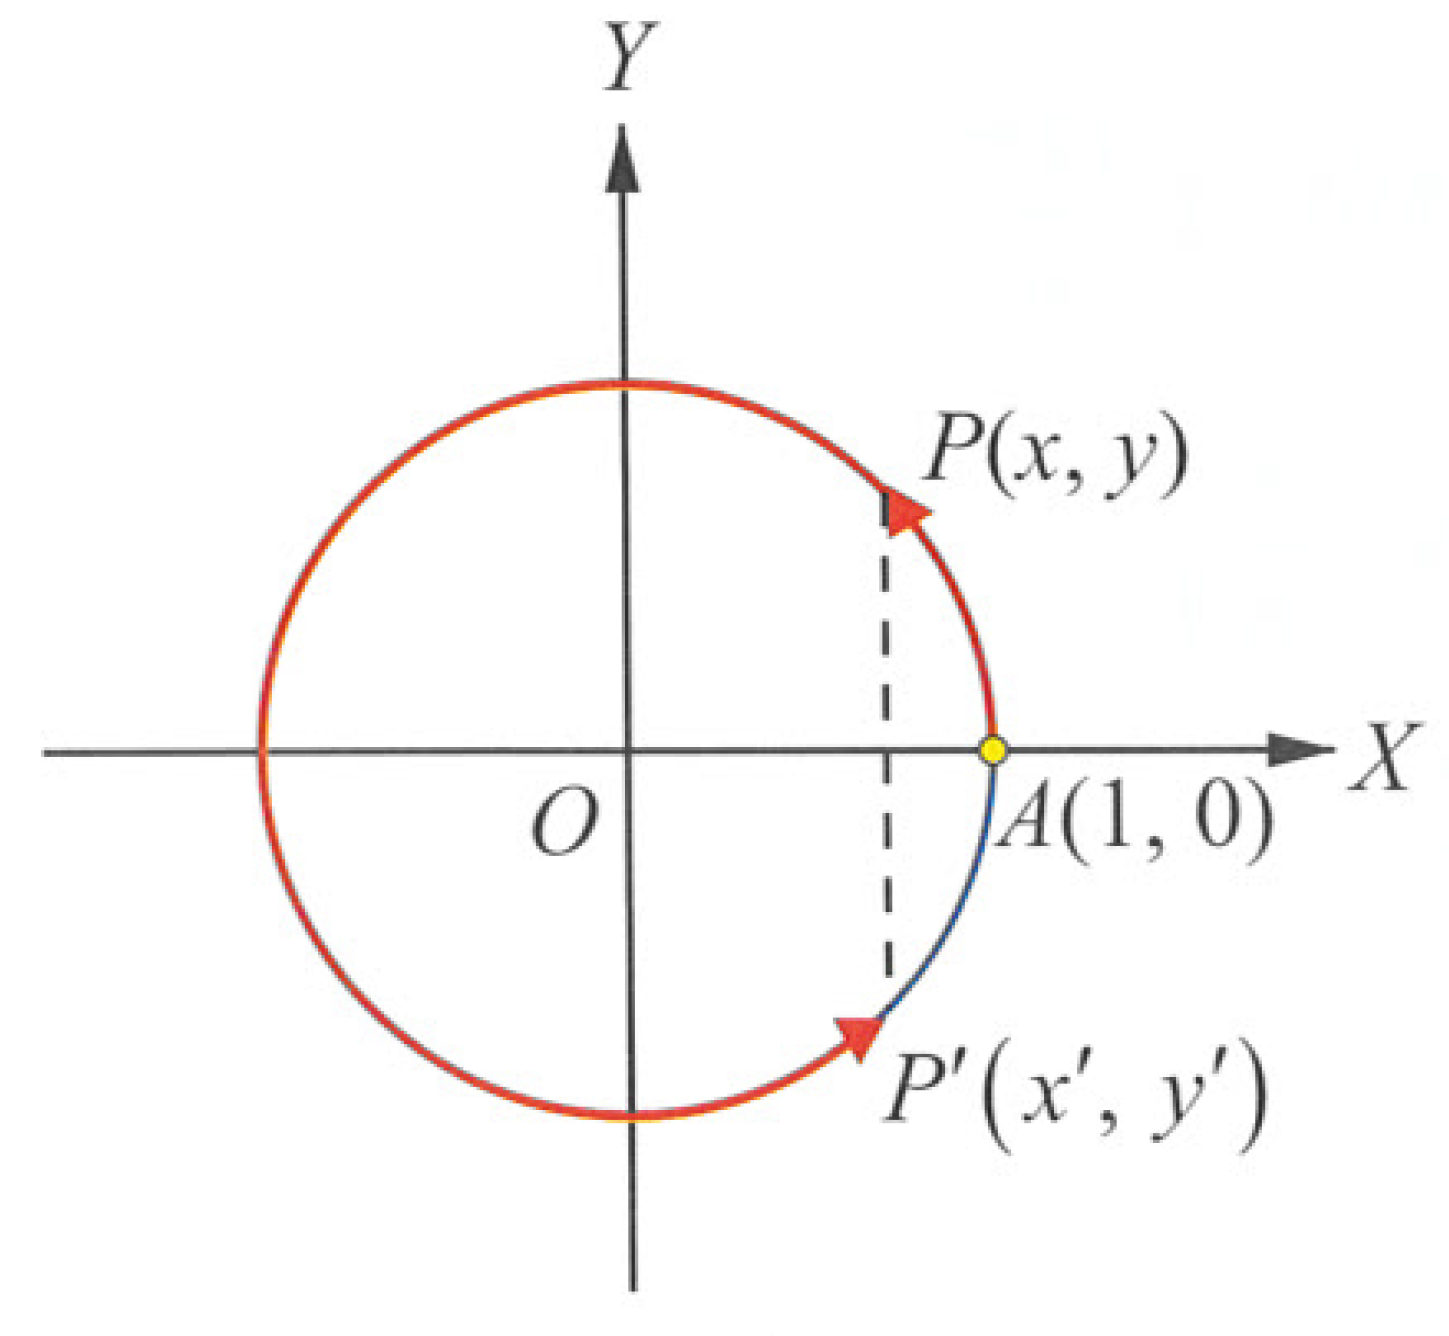
\includegraphics[scale=0.40]{10} 
	\caption{} 
	\label{Figure10} 
\end{figure}

\noindent ให้ $P^{\prime}(x^{\prime}, y^{\prime})$ เป็นจุดปลายส่วนโค้งที่ยาว $\theta$ หน่วย 
\\
ดังนั้น $y^{\prime} = \sin\theta$ และ $x^{\prime} = \cos\theta$
\\
ให้ $\alpha = 2\pi - \theta$ จะได้ว่า $0 < \alpha < \dfrac{\pi}{2}$

\vspace{0.5em}
\noindent เนื่องจากเส้นรอบวงของวงกลมหนึ่งหน่วยยาว $2\pi$ หน่วย ดังนั้น ส่วนโค้งจากจุดปลาย $P^{\prime}$ ย้อนกลับมายังแกน $X$ ที่จุด $(1,0)$ ย่อมยาว $\alpha$ หน่วย 
\\
เมื่อให้จุด $P(x, y)$ เป็นภาพสะท้อนของจุด $P^{\prime}(x^{\prime}, y^{\prime})$ โดยมีแกน $X$ เป็นเส้นสะท้อน 
\\
จะได้ว่าส่วนโค้ง $AP$ ในจตุภาคที่ 1 ยาว $\alpha$ หน่วย และมีความสัมพันธ์ของพิกัดสะท้อนเป็น $y^{\prime} = -y$ และ $x^{\prime} = x$

\vspace{0.5em}
\noindent เนื่องจากจุด $P(x, y)$ เป็นจุดปลายส่วนโค้งที่ยาว $\alpha$ หน่วยในจตุภาคที่ 1
\\
ดังนั้น 
$$y = \sin\alpha \quad \text{และ} \quad x = \cos\alpha$$

\vspace{0.3em}
\noindent เมื่อพิจารณาความสัมพันธ์ร่วมกับพิกัดจุดสะท้อนข้ามแกน $X$ จะได้ว่า
$$y^{\prime} = -y \implies \sin\theta = -\sin\alpha$$
$$\sin\left(2\pi - \alpha\right) = -\sin\alpha$$
\\[0.3em]
และ
$$x^{\prime} = x \implies \cos\theta = \cos\alpha$$
$$\cos\left(2\pi - \alpha\right) = \cos\alpha$$

\vspace{1em}
\noindent สรุปความสัมพันธ์เชิงเรขาคณิตสำหรับจตุภาคที่ 4 ได้ดังนี้
$$\sin\left(2\pi - \alpha\right) = -\sin\alpha \quad \text{เมื่อ} \quad 0 < \alpha < \dfrac{\pi}{2}$$
$$\cos\left(2\pi - \alpha\right) = \cos\alpha \quad \text{เมื่อ} \quad 0 < \alpha < \dfrac{\pi}{2}$$

\begin{examplebox}
จงหาค่าของฟังก์ชันไซน์และโคไซน์ของ $\dfrac{11 \pi}{6}$
\end{examplebox}
\solution

\newpage

\section{ฟังก์ชันตรีโกณมิติอื่น ๆ}
นอกจากฟังก์ชันไซน์และโคไซน์ดังกล่าวแล้ว ยังมีฟังก์ชันตรีโกณมิติที่สำคัญอีกหลายฟังก์ชัน ดังต่อไปนี้

\vspace{0.5em}
ฟังก์ชันแทนเจนต์ (tangent function) เขียนแทนด้วย $\tan$ (อ่านว่า แทน) ฟังก์ชันเซแคนต์ (secant function) เขียนแทนด้วย $\sec$ (อ่านว่า เซก) ฟังก์ชันโคเซแคนต์ (cosecant function) เขียนแทนด้วย $\operatorname{cosec}$ หรือ $\csc$ (อ่านว่า โคเซก) และฟังก์ชันโคแทนเจนต์ (cotangent function) เขียนแทนด้วย $\cot$ (อ่านว่า คอต)

\vspace{0.5em}
\noindent นิยามค่าของฟังก์ชันตรีโกณมิติเหล่านี้ โดยอาศัยค่าของฟังก์ชันไซน์และโคไซน์ ดังนี้

\begin{definitionbox}
	สำหรับจำนวนจริง $\theta$ ใด ๆ จะได้นิยามความสัมพันธ์ทางตรีโกณมิติดังต่อไปนี้
	$$\tan\theta = \dfrac{\sin\theta}{\cos\theta} \quad \text{เมื่อ} \quad \cos\theta \neq 0$$
	$$\sec\theta = \dfrac{1}{\cos\theta} \quad \text{เมื่อ} \quad \cos\theta \neq 0$$
	$$\operatorname{cosec}\theta = \dfrac{1}{\sin\theta} \quad \text{เมื่อ} \quad \sin\theta \neq 0$$
	$$\cot\theta = \dfrac{\cos\theta}{\sin\theta} \quad \text{เมื่อ} \quad \sin\theta \neq 0$$
\end{definitionbox}

\vspace{1em}
\noindent จากบทนิยามข้างต้น จะได้รายละเอียดของโดเมนและเรนจ์ดังนี้
\begin{enumerate}
	\item โดเมนของฟังก์ชัน $\tan$ และ $\sec$ คือ $\mathbb{R} - \left\{x \;\middle|\; x = \dfrac{(2n+1)\pi}{2}, \; n \in \mathbb{Z}\right\}$
	\item โดเมนของฟังก์ชัน $\cot$ และ $\operatorname{cosec}$ คือ $\mathbb{R} - \{x \mid x = n\pi, \; n \in \mathbb{Z}\}$
	\item เรนจ์ของฟังก์ชัน $\tan$ และ $\cot$ คือ $\mathbb{R}$
	\item เรนจ์ของฟังก์ชัน $\sec$ และ $\operatorname{cosec}$ คือ $\mathbb{R} - \{x \mid -1 < x < 1\}$
\end{enumerate}

\vspace{1.5em}
\noindent นอกจากนี้ สามารถหาความสัมพันธ์เชื่อมโยงระหว่างฟังก์ชันตรีโกณมิติต่าง ๆ ได้เพิ่มเติม เช่น
$$\cot\theta = \dfrac{1}{\tan\theta} \quad \text{เมื่อ} \quad \tan\theta \neq 0$$
$$1 + \tan^2\theta = \sec^2\theta \quad \text{เมื่อ} \quad \cos\theta \neq 0$$
$$1 + \cot^2\theta = \operatorname{cosec}^2\theta \quad \text{เมื่อ} \quad \sin\theta \neq 0$$

\newpage
\noindent เอกลักษณ์และความสัมพันธ์เหล่านี้ สามารถพิสูจน์ข้อเท็จจริงได้ดังนี้

\vspace{0.5em}
\noindent\textbf{(1) การพิสูจน์ความสัมพันธ์} $\cot\theta = \dfrac{1}{\tan\theta}$ เมื่อ $\tan\theta \neq 0$
$$\cot\theta = \dfrac{\cos\theta}{\sin\theta}$$
$$\cot\theta = \dfrac{1}{\;\dfrac{\sin\theta}{\cos\theta}\;}$$
$$\cot\theta = \dfrac{1}{\tan\theta}$$

\vspace{1em}
\noindent\textbf{(2) การพิสูจน์ความสัมพันธ์} $1 + \tan^2\theta = \sec^2\theta$ เมื่อ $\cos\theta \neq 0$
$$1 + \tan^2\theta = 1 + \dfrac{\sin^2\theta}{\cos^2\theta}$$
$$1 + \tan^2\theta = \dfrac{\cos^2\theta + \sin^2\theta}{\cos^2\theta}$$
$$\text{เนื่องจาก } \cos^2\theta + \sin^2\theta = 1 \text{ จะได้ว่า}$$
$$1 + \tan^2\theta = \dfrac{1}{\cos^2\theta}$$
$$1 + \tan^2\theta = \sec^2\theta$$

\vspace{1.5em}
\noindent สำหรับความสัมพันธ์อื่น ๆ ที่ไม่ได้แสดงการพิสูจน์ไว้ สามารถพิสูจน์ได้ในทำนองเดียวกัน โดยความสัมพันธ์ระหว่างฟังก์ชันตรีโกณมิติต่าง ๆ นอกเหนือจากที่กล่าวมาข้างต้น จะนำไปกล่าวถึงโดยละเอียดในหัวข้อถัดไป

\vspace{0.5em}
\noindent ค่าของฟังก์ชันตรีโกณมิติที่กำหนดใหม่ทั้งหมด สามารถหาได้จากการเทียบเคียงกับฟังก์ชันไซน์และโคไซน์ ดังแสดงในตัวอย่างต่อไปนี้

\begin{examplebox}
จงหาค่าของฟังก์ชันตรีโกณมิติทุกฟังก์ชันของ $\dfrac{\pi}{3}$
\end{examplebox}
\solution

\newpage
\subsection*{ตารางแสดงค่าของฟังก์ชันตรีโกณมิติของจำนวนจริง $\theta$ บางจำนวน เมื่อ $0 \leq \theta \leq \dfrac{\pi}{2}$}

\begin{figure}[H] 
	\centering 
	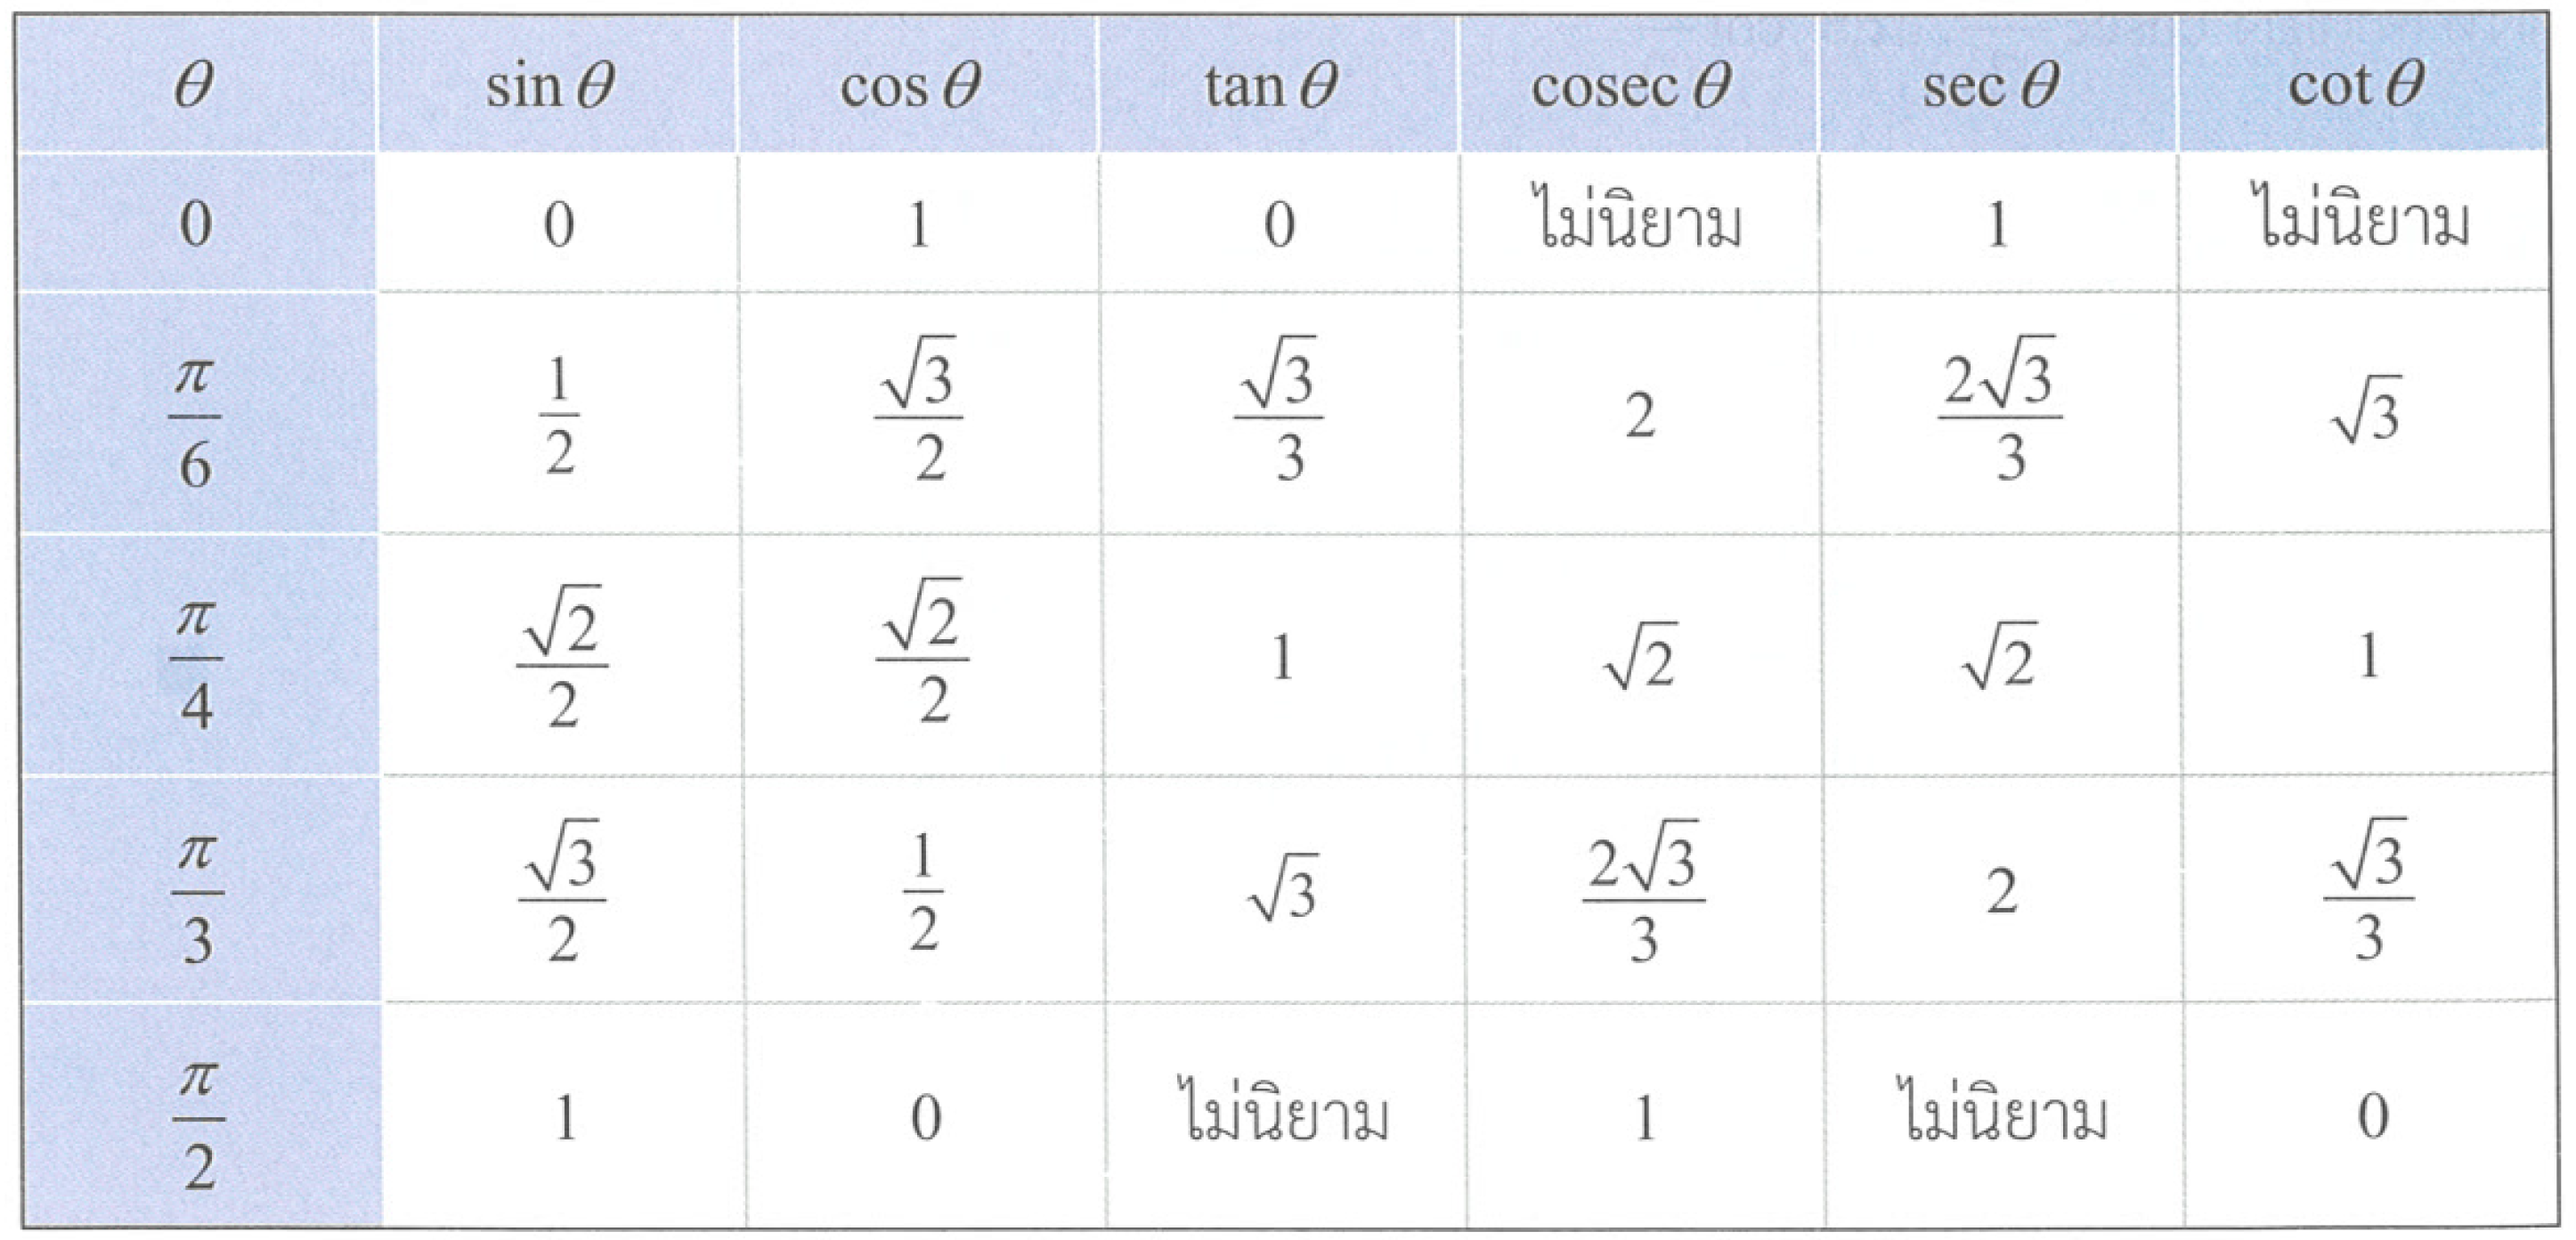
\includegraphics[scale=0.35]{11} 
	\caption{} 
	\label{Figure11} 
\end{figure}

\begin{examplebox}
	จงหาค่าของ $\tan\pi$ และ $\sec\pi$
\end{examplebox}
\solution
\vspace{5cm}

\begin{examplebox}
	จงหาค่าของ $\tan\left(-\dfrac{3\pi}{2}\right)$ และ $\sec\left(-\dfrac{3\pi}{2}\right)$
\end{examplebox}
\solution
\vspace{5cm}

\begin{examplebox}
	จงหาค่าของ $\operatorname{cosec}\left(\dfrac{5\pi}{2}\right)$ และ $\cot\left(\dfrac{5\pi}{2}\right)$
\end{examplebox}
\solution
\vspace{5cm}

\begin{examplebox}
	จงหาค่าของ $\operatorname{cosec}3\pi$ และ $\operatorname{\cot}3\pi$
	\end{examplebox}
	\solution
	\vspace{5cm}
	
\begin{examplebox}
จงหาค่าของ $\sin\left(\dfrac{\pi}{3}\right)\cos\left(\dfrac{5\pi}{6}\right) + \sin\left(\dfrac{4\pi}{3}\right)\cos\left(\dfrac{\pi}{6}\right)$
\end{examplebox}
\solution
\newpage

\begin{examplebox}
	จงแสดงว่า $\tan(n\pi + \theta) = \tan\theta$ เมื่อ $n$ เป็นจำนวนเต็มใด ๆ
\end{examplebox}
\solution 
\vspace{0.5em}\\
\noindent\textbf{กรณีที่ 1:} เมื่อ $n$ เป็นจำนวนคู่
\\
สมมติให้เขียน $n = 2k$ เมื่อ $k$ เป็นจำนวนเต็มใด ๆ
\\
ดังนั้น จะได้ว่า $\tan(n\pi + \theta) = \tan(2k\pi + \theta)$ ซึ่งกระจายตามนิยามได้เป็น
$$\tan(2k\pi + \theta) = \dfrac{\sin(2k\pi + \theta)}{\cos(2k\pi + \theta)}$$
จากสมบัติการวนรอบรอบวงกลมหนึ่งหน่วย ($2k\pi$) จะลดรูปได้เป็น
$$\tan(2k\pi + \theta) = \dfrac{\sin\theta}{\cos\theta}$$
$$\tan(2k\pi + \theta) = \tan\theta$$

\vspace{1.5em}
\noindent\textbf{กรณีที่ 2:} เมื่อ $n$ เป็นจำนวนคี่
\\
สมมติให้เขียน $n = 2k + 1$ เมื่อ $k$ เป็นจำนวนเต็มใด ๆ
\\
ดังนั้น จะได้ว่า $\tan(n\pi + \theta) = \tan((2k + 1)\pi + \theta)$ ซึ่งจัดรูปมุมสัมพันธ์ได้เป็น
$$\tan((2k + 1)\pi + \theta) = \tan(2k\pi + \pi + \theta)$$
จากสมบัติการวนรอบรอบวงกลมหนึ่งหน่วย สามารถตัดพจน์ $2k\pi$ ออกได้เหลือเพียง
$$\tan((2k + 1)\pi + \theta) = \tan(\pi + \theta)$$
เมื่อกระจายตามนิยามอัตราส่วนตรีโกณมิติ จะได้
$$\tan(\pi + \theta) = \dfrac{\sin(\pi + \theta)}{\cos(\pi + \theta)}$$
และจากสมบัติพิกัดภาพสะท้อนในจตุภาคที่ 3 (Quadrant III) จะเปลี่ยนรูปพจน์ได้ดังนี้
$$\tan(\pi + \theta) = \dfrac{-\sin\theta}{-\cos\theta}$$
$$\tan(\pi + \theta) = \dfrac{\sin\theta}{\cos\theta} = \tan\theta$$

\vspace{1.5em}
\noindent จากผลการพิสูจน์ทั้งสองกรณี จึงสรุปได้ว่า
$$\tan(n\pi + \theta) = \tan\theta \quad \text{เมื่อ } n \text{ เป็นจำนวนเต็มใด ๆ}$$

\section{ฟังก์ชันตรีโกณมิติของมุม}
\subsection*{มุมและการวัดมุม}

\noindent กำหนดส่วนของเส้นตรง $AP$ ต้องการสร้างมุม $P\hat{A}Q$ ให้มีขนาด $30$ องศา โดยใช้โพรแทรกเตอร์วัดขนาดของมุม ทำได้โดยวางโพรแทรกเตอร์ทับส่วนของเส้นตรง $AP$ ซึ่งสามารถวัดขนาดของมุมที่ต้องการสร้างได้ $2$ แบบ คือ วัดในทิศทางทวนเข็มนาฬิกา และวัดในทิศทางตามเข็มนาฬิกา ดังรูป

\begin{figure}[H] 
	\centering 
	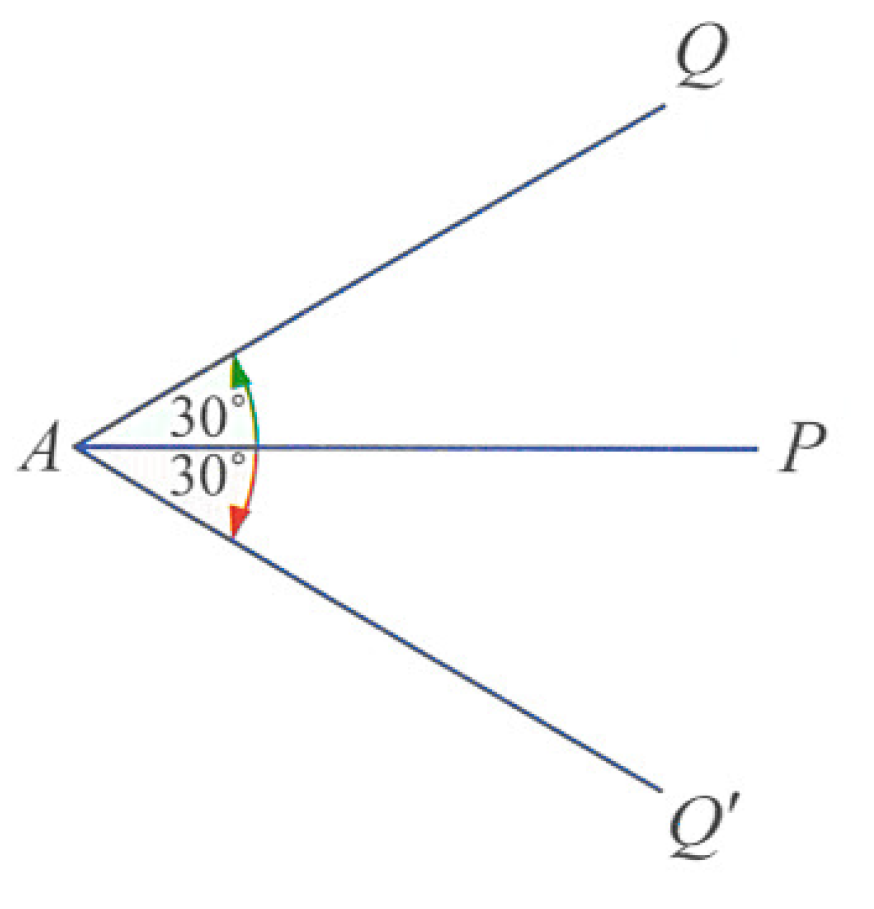
\includegraphics[scale=0.45]{12} 
	\caption{} 
	\label{Figure12} 
\end{figure}

\noindent เรียกจุด $A$ ว่า \textbf{จุดยอด (vertex)} ของมุม 
\\
เรียกส่วนของเส้นตรง $AP$ ว่า \textbf{ด้านเริ่มต้น (initial side)} ของมุม 
\\
เรียกส่วนของเส้นตรง $AQ$ และ $AQ'$ ว่า \textbf{ด้านสิ้นสุด (terminal side)} ของมุม

\vspace{0.5em}
\noindent ดังนั้น การวัดขนาดของมุมทำได้โดยการวัดจากด้านเริ่มต้นไปยังด้านสิ้นสุด สำหรับการบอกขนาดของมุมมีข้อตกลงว่า ถ้าวัดมุมในทิศทางทวนเข็มนาฬิกา จะแสดงขนาดของมุมด้วยจำนวนจริงบวก แต่ถ้าวัดมุมในทิศทางตามเข็มนาฬิกา จะแสดงขนาดของมุมด้วยจำนวนจริงลบ

\vspace{0.5em}
\noindent หน่วยในการวัดมุมที่รู้จักกันแล้ว คือ\textbf{ องศา (degree)} เขียนแทนด้วยสัญลักษณ์ $^{\circ}$ โดยมุมที่ด้านเริ่มต้นและด้านสิ้นสุดทับกันพอดีมีขนาด $0$ องศา หรือ $360$ องศา และแบ่งหน่วยองศาออกเป็นหน่วยย่อยคือ ลิปดา ($'$) และพิลิปดา ($''$) ตามความสัมพันธ์ดังนี้
$$
\begin{aligned}
	1^{\circ} &= 60' \\
	1' &= 60''
\end{aligned}
$$

\vspace{1em}
\noindent หน่วยวัดมุมที่สำคัญอีกหน่วยหนึ่งในทางคณิตศาสตร์ระดับสูงคือ \textbf{เรเดียน (radian)}

\begin{figure}[H] 
	\centering 
	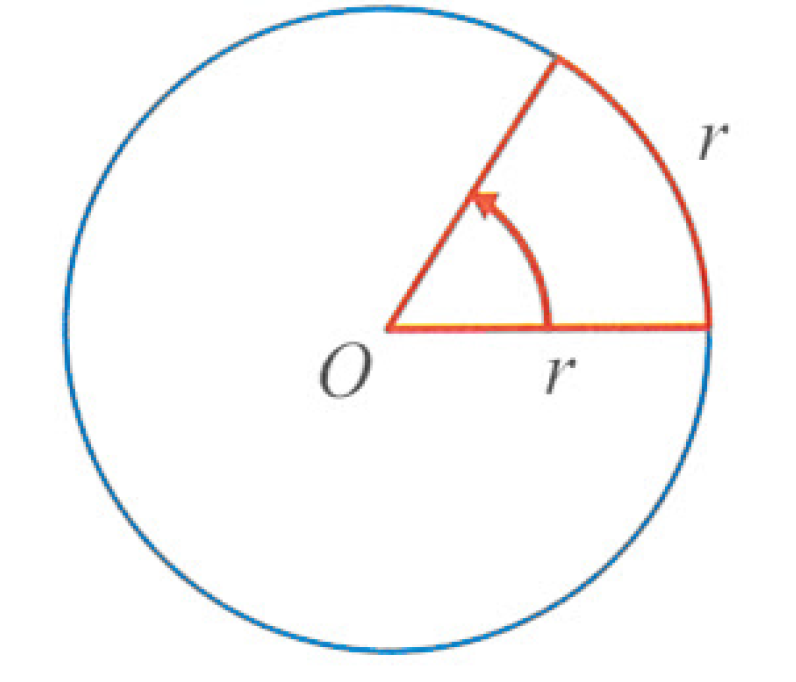
\includegraphics[scale=0.33]{13} 
	\caption{} 
	\label{Figure13} 
\end{figure}

\vspace{0.5em}
\textbf{ มุมที่จุดศูนย์กลางของวงกลมซึ่งรองรับด้วยส่วนโค้งของวงกลมที่ยาวเท่ากับรัศมีของวงกลมนั้น เป็นมุมที่มีขนาด $1$ เรเดียน}

\vspace{0.5em}
\noindent เนื่องจากวงกลมที่มีรัศมียาว $r$ หน่วย จะมีเส้นรอบวงยาว $2\pi r$ หน่วย 
\\
ดังนั้น มุมที่จุดศูนย์กลางของวงกลมซึ่งรองรับด้วยส่วนโค้งของวงกลมที่ยาว $2\pi r$ หน่วย จึงมีขนาด $\dfrac{2\pi r}{r} = 2\pi$ เรเดียน และมุมที่จุดศูนย์กลางของวงกลมซึ่งรองรับด้วยส่วนโค้งครึ่งวงกลมที่ยาว $\pi r$ หน่วย จะมีขนาด $\dfrac{\pi r}{r} = \pi$ เรเดียน

\vspace{0.5em}
\noindent ในกรณีทั่วไป สำหรับมุมที่จุดศูนย์กลางของวงกลมที่มีรัศมียาว $r$ หน่วย ซึ่งรองรับด้วยส่วนโค้งของวงกลมที่ยาว $a$ หน่วย จะมีขนาด $\dfrac{a}{r}$ เรเดียน และถ้าให้ขนาดของมุมดังกล่าวเป็น $\theta$ เรเดียน จะได้ความสัมพันธ์เป็น
$$\theta = \dfrac{a}{r}$$

\noindent เนื่องจากมุมที่จุดศูนย์กลางของวงกลมที่มีรัศมียาว $r$ หน่วย มีขนาด $2\pi$ เรเดียน หรือ 360 องศา ดังนั้น ย่อมได้ความสัมพันธ์ว่า

\vspace{0.5em}
\centerline{\textbf{360 องศา เท่ากับ $2\pi$ เรเดียน}}
\vspace{0.5em}

\noindent หรือสรุปในรูปอย่างง่ายได้ว่า \textbf{180 องศา เท่ากับ $\pi$ เรเดียน}
\\
ดังนั้น จึงได้ข้อสรุปในการแปลงหน่วยมุมดังนี้
$$1 \text{ องศา} = \dfrac{\pi}{180} \text{ เรเดียน} \approx 0.01745 \text{ เรเดียน}$$
และ
$$1 \text{ เรเดียน} = \dfrac{180}{\pi} \text{ องศา} \approx 57.3^{\circ} \quad \text{หรือ} \quad 57^{\circ}18'$$

\vspace{1em}
\noindent โดยทั่วไปการเขียนขนาดของมุมที่มีหน่วยเป็นเรเดียนมักจะไม่เขียนหน่วยกำกับไว้ ดังนั้น ถ้ากล่าวถึงขนาดของมุมโดยไม่มีหน่วยกำกับ ให้ถือว่ามุมนั้นมีหน่วยเป็นเรเดียนเสมอ

\vspace{0.5em}
\noindent จากความสัมพันธ์ระหว่างขนาดของมุมในหน่วยองศาและหน่วยเรเดียนที่กล่าวมาข้างต้น จะเห็นว่าเมื่อเราทราบขนาดของมุมในหน่วยใดหน่วยหนึ่งแล้ว จะสามารถคำนวณเปลี่ยนเทียบขนาดของมุมนั้นในอีกหน่วยหนึ่งได้ ดังจะแสดงในตัวอย่างต่อไปนี้

\begin{examplebox}
	มุมที่มีขนาด $\dfrac{1}{2}$ เรเดียน มีขนาดกี่องศา
\end{examplebox}
\solution
\vspace{7cm}

\begin{examplebox}
	มุมที่มีขนาด $75$ องศา มีขนาดกี่เรเดียน
\end{examplebox}
\solution

\newpage
\subsection*{ฟังก์ชันตรีโกณมิติของมุม}
\noindent ฟังก์ชันตรีโกณมิติที่กล่าวมาในบทเรียนก่อนหน้านี้นั้น เป็นฟังก์ชันของจำนวนจริง ต่อไปนี้จะพิจารณาขยายแนวคิดไปถึง \textbf{ฟังก์ชันตรีโกณมิติของมุม}

\vspace{0.5em}
\noindent เมื่อจุดยอดของมุมอยู่ที่จุด $(0,0)$ และด้านเริ่มต้นของมุมนั้นทาบไปตามแกน $X$ ทางบวก จะกล่าวว่า มุมนั้นอยู่ใน \textbf{ตำแหน่งมาตรฐาน (standard position)}

\vspace{0.5em}
\noindent สมมติว่า มุมหนึ่งมีขนาด $\theta$ เรเดียน อยู่ในตำแหน่งมาตรฐาน ดังรูป

\begin{figure}[H] 
	\centering 
	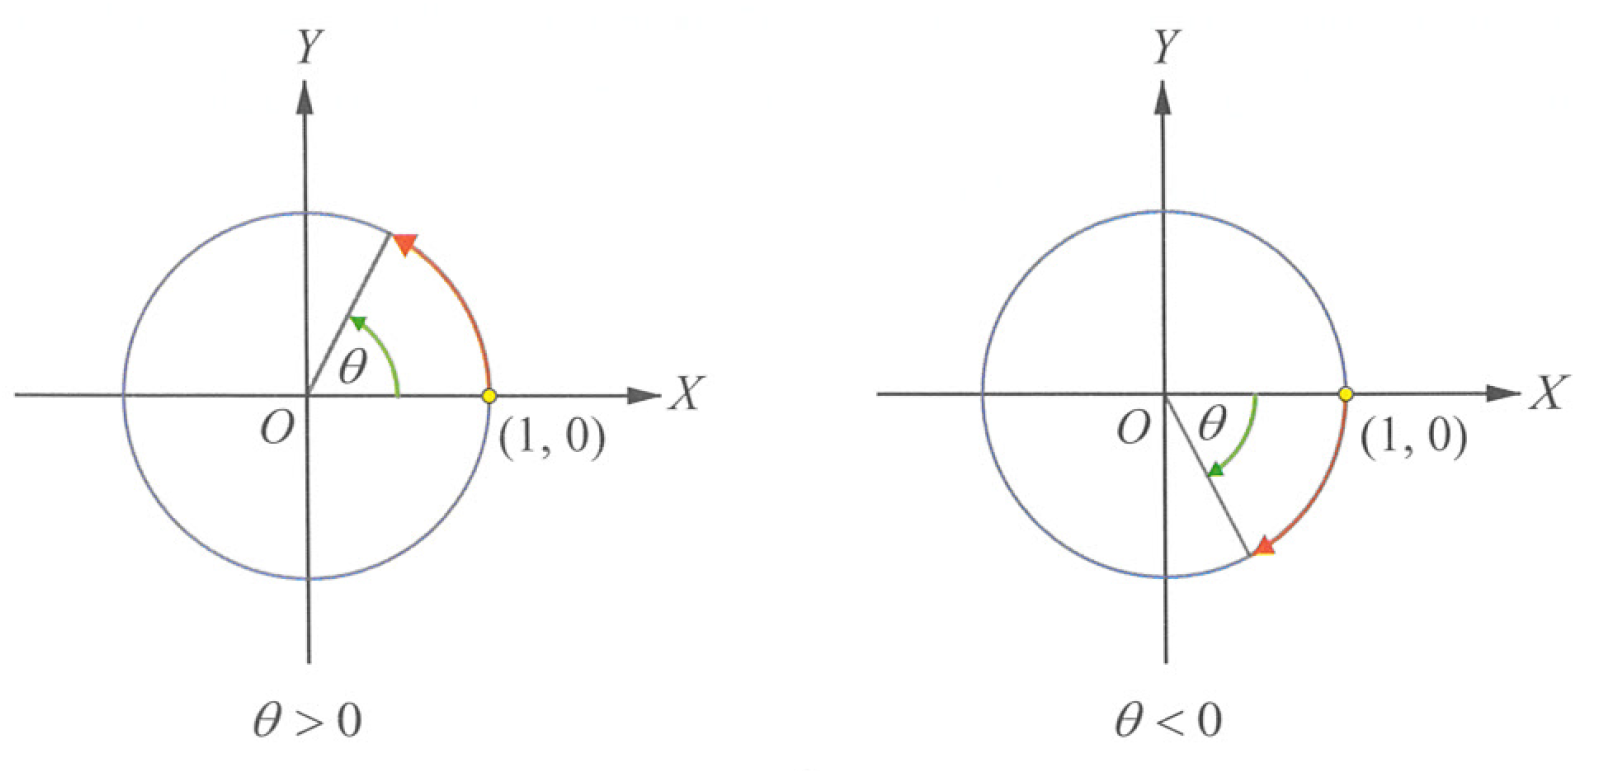
\includegraphics[scale=0.6]{14} 
	\caption{มุมขนาด $\theta$ เรเดียน ในตำแหน่งมาตรฐานบนระบบพิกัดฉาก} 
	\label{Figure14} 
\end{figure}

\vspace{0.5em}
\noindent เนื่องจากส่วนโค้งของวงกลมหนึ่งหน่วยที่รองรับมุมที่จุดศูนย์กลางขนาด $1$ เรเดียนนั้น ยาว $1$ หน่วย ดังนั้น ส่วนโค้งของวงกลมหนึ่งหน่วยที่รองรับมุมที่จุดศูนย์กลางขนาด $\theta$ เรเดียน จึงยาว $\theta$ หน่วยด้วย

\vspace{0.5em}
\noindent จะเห็นว่า จุดที่ด้านสิ้นสุดของมุมขนาด $\theta$ เรเดียน ตัดกับวงกลมหนึ่งหน่วยนั้นมีเพียงจุดเดียว และย่อมเป็นจุดเดียวกันกับจุดปลายส่วนโค้งที่วัดจากจุด $(1,0)$ เป็นระยะทาง $|\theta|$ หน่วย ในทิศทางที่สอดคล้องตามเครื่องหมายของมุม $\theta$ 

\vspace{0.5em}
\noindent เช่น จุดที่ด้านสิ้นสุดของมุมขนาด $-\dfrac{\pi}{4}$ เรเดียน ตัดกับวงกลมหนึ่งหน่วย คือ จุด $\left(\dfrac{\sqrt{2}}{2}, -\dfrac{\sqrt{2}}{2}\right)$ ซึ่งเป็นจุดพิกัดเดียวกันกับจุดปลายส่วนโค้งที่วัดระยะจากจุด $(1,0)$ ไปในทิศทางตามเข็มนาฬิกาเป็นระยะทางยาว $\dfrac{\pi}{4}$ หน่วย

\vspace{0.5em}
\noindent ดังนั้น เมื่อกำหนดมุมขนาด $\theta$ เรเดียนให้หนึ่งมุม จะสามารถหาจุดที่ด้านสิ้นสุดของมุมนั้นตัดกับวงกลมหนึ่งหน่วยได้เพียงจุดเดียวเสมอ และจุดนั้นจะเป็นจุดปลายส่วนโค้งที่ยาว $|\theta|$ หน่วยด้วย หรือกล่าวได้ว่าส่วนโค้งของวงกลมหนึ่งหน่วยที่รองรับมุม $\theta$ เรเดียน จะยาว $|\theta|$ หน่วย 

\vspace{0.5em}
\noindent สังเกตได้ว่า ไม่ว่าจะใช้วิธีวัดมุมหรือวัดความยาวส่วนโค้งของวงกลม จุดที่ด้านสิ้นสุดของมุมตัดกับวงกลมหนึ่งหน่วยจะเป็นจุดเดียวกันกับจุดปลายส่วนโค้งทุกประการ

\vspace{1em}
\noindent จากข้อเท็จจริงทางเรขาคณิตนี้ จึงสรุปได้ว่า \textbf{ไม่ว่าจะนิยามฟังก์ชันตรีโกณมิติในแง่ของมุม หรือในแง่ของความยาวส่วนโค้งของวงกลมหนึ่งหน่วยที่รองรับมุม ค่าของฟังก์ชันตรีโกณมิติของจำนวนเหล่านั้นจะเท่ากันเสมอ} เช่น พจน์ $\cos\theta$ อาจหมายถึงค่า $\cos$ ของมุมที่มีขนาด $\theta$ เรเดียน หรือค่า $\cos$ ของจำนวนจริง $\theta$ ก็ได้ตามบริบทแวดล้อม

\vspace{1em}
\noindent ในการหาค่าของฟังก์ชันตรีโกณมิติของมุมที่มีหน่วยเป็นองศานั้น อาจหาได้โดยการคำนวณเปลี่ยนหน่วยวัดขนาดของมุมจากหน่วยองศาให้เป็นหน่วยเรเดียนก่อน แล้วจึงทำการหาค่าของฟังก์ชันนั้นในลักษณะเดียวกันกับการหาค่าของฟังก์ชันตรีโกณมิติของจำนวนจริงทั่ว ๆ ไป

\begin{examplebox}
จงหาค่าของ $\sin 60^{\circ}$
\end{examplebox}
\solution
\vspace{7cm}

\begin{examplebox}
จงหาค่าของ $\sec \left(-405^{\circ}\right)$
\end{examplebox}
\solution
\newpage

\subsection*{ฟังก์ชันตรีโกณมิติของมุมของรูปสามเหลี่ยมมุมฉาก}

ประโยชน์ที่สำคัญประการหนึ่งของฟังก์ชันตรีโกณมิติ คือ การนำไปใช้ในการหาส่วนต่าง ๆ ของรูปสามเหลี่ยม ต่อไปนี้จะพิจารณาฟังก์ชันตรีโกณมิติของมุมของรูปสามเหลี่ยมมุมฉาก

\vspace{0.5em}
\noindent กำหนดรูปสามเหลี่ยมมุมฉาก $ABC$ ที่มี $A\hat{C}B$ เป็นมุมฉาก ดังนั้น $B\hat{A}C < 90^{\circ}$
\\
ให้ $a, b$ และ $c$ เป็นความยาวของด้านตรงข้ามมุม $A, B$ และ $C$ ของรูปสามเหลี่ยม $ABC$ ตามลำดับ
\\
ให้ $B\hat{A}C$ อยู่ในตำแหน่งมาตรฐาน และส่วนโค้งของวงกลมหนึ่งหน่วยที่รองรับมุม $A$ คือ ส่วนโค้ง $FD$ ดังรูป

\begin{figure}[H] 
	\centering 
	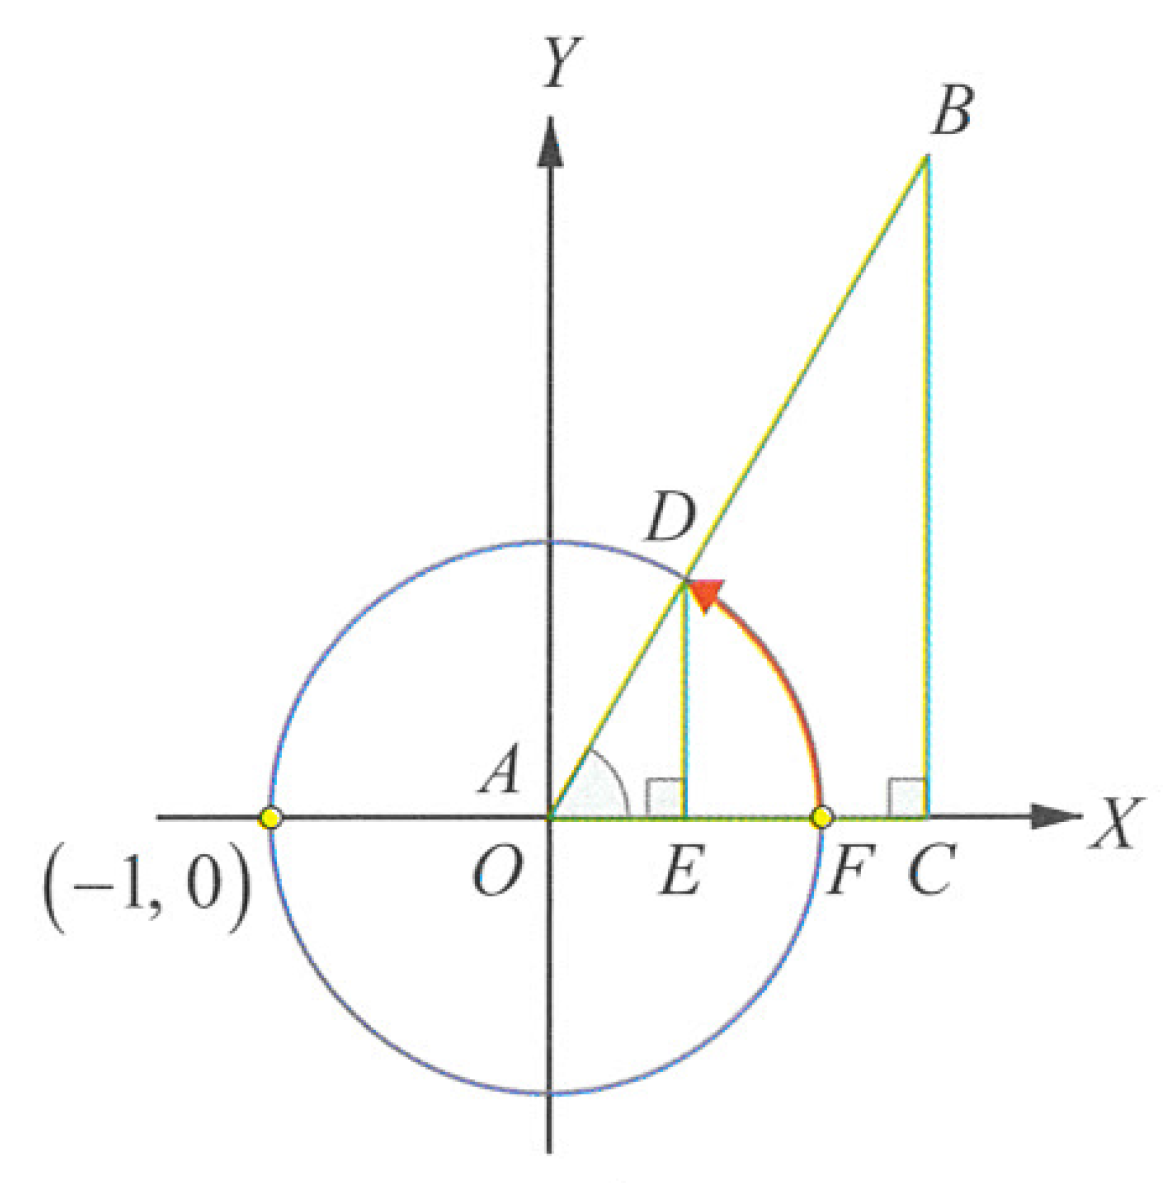
\includegraphics[scale=0.5]{15} 
	\caption{} 
	\label{Figure15} 
\end{figure}

\noindent จากนิยามของฟังก์ชันตรีโกณมิติบนวงกลมหนึ่งหน่วย จะได้ว่า
\\
$\sin A = \sin(\text{ความยาวส่วนโค้ง } FD) = DE$
\\
$\cos A = \cos(\text{ความยาวส่วนโค้ง } FD) = AE$

\vspace{0.5em}
\noindent เนื่องจากรูปสามเหลี่ยมมุมฉาก $ADE$ เป็นรูปสามเหลี่ยมที่คล้ายกับรูปสามเหลี่ยม $ABC$
\\
จากสมบัติของรูปสามเหลี่ยมคล้าย จะได้อัตราส่วนความยาวด้านที่สมนัยกันดังนี้
$$\dfrac{DE}{AD} = \dfrac{BC}{AB} \quad \text{และ} \quad \dfrac{AE}{AD} = \dfrac{AC}{AB}$$
แต่เนื่องจากรัศมีของวงกลมหนึ่งหน่วยทำให้ $AD = 1$
\\
ดังนั้น ย่อมได้ว่า $DE = \dfrac{BC}{AB} = \dfrac{a}{c}$ และ $AE = \dfrac{AC}{AB} = \dfrac{b}{c}$

\vspace{0.5em}
\noindent นั่นคือ $\sin A = \dfrac{a}{c}$, $\cos A = \dfrac{b}{c}$ และสำหรับการหาค่าฟังก์ชันแทนเจนต์ จะได้ความสัมพันธ์เป็น
$$\tan A = \dfrac{\sin A}{\cos A} = \dfrac{\;\dfrac{a}{c}\;}{\;\dfrac{b}{c}} = \dfrac{a}{b}$$

\vspace{1em}
\noindent จากความสัมพันธ์ของรูปสามเหลี่ยมคล้ายข้างต้น จึงนำมาสรุปเป็นนิยามอัตราส่วนตรีโกณมิติบนรูปสามเหลี่ยมมุมฉากได้ดังนี้
$$\sin A = \dfrac{\text{ความยาวของด้านตรงข้ามมุม } A}{\text{ความยาวของด้านตรงข้ามมุมฉาก}}$$
$$\cos A = \dfrac{\text{ความยาวของด้านประชิดมุม } A}{\text{ความยาวของด้านตรงข้ามมุมฉาก}}$$
$$\tan A = \dfrac{\text{ความยาวของด้านตรงข้ามมุม } A}{\text{ความยาวของด้านประชิดมุม } A}$$

\vspace{1em}
\noindent ส่วนค่าของฟังก์ชันโคเซแคนต์ ฟังก์ชันเซแคนต์ และฟังก์ชันโคแทนเจนต์ของมุม $A$ จะเป็นส่วนกลับของค่าของฟังก์ชันไซน์ ฟังก์ชันโคไซน์ และฟังก์ชันแทนเจนต์ ตามลำดับ 

\vspace{0.5em}
\noindent สมการอัตราส่วนส่วนปลายเหล่านี้นั้น มีประโยชน์อย่างมากในการคำนวณหาส่วนต่าง ๆ ของรูปสามเหลี่ยมมุมฉาก ดังจะแสดงให้เห็นในตัวอย่างต่อไปนี้

\newpage
\begin{examplebox}
	รูปสามเหลี่ยมมุมฉาก $ABC$ มี $A\hat{C}B$ เป็นมุมฉาก ด้าน $AC$ ยาว $4$ หน่วย และมุม $A$ มีขนาด $30^{\circ}$ จงหาความยาวของด้าน $AB$ และ $BC$
\end{examplebox}
\solution 
\begin{figure}[H] 
	\centering 
	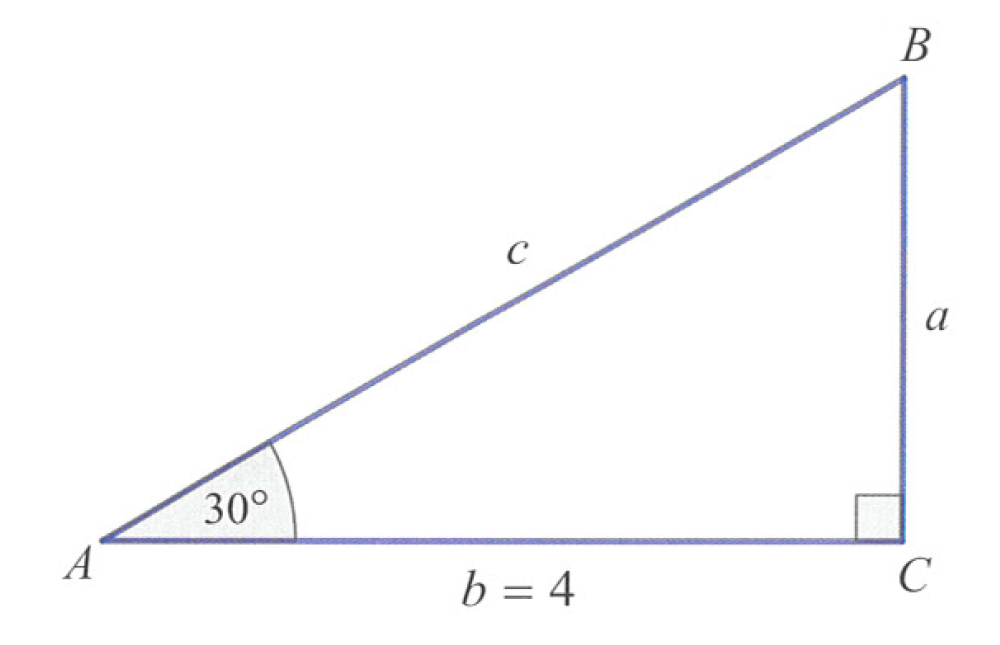
\includegraphics[scale=0.5]{16} 
	\caption{} 
	\label{Figure16} 
\end{figure}
\newpage

\begin{examplebox}
	ให้มุม $A$ เป็นมุมแหลม และ $\sin A = \dfrac{3}{7}$ จงหาค่าของฟังก์ชันตรีโกณมิติต่าง ๆ ที่เหลือของมุม $A$
\end{examplebox}
\solution 
\begin{figure}[H] 
	\centering 
	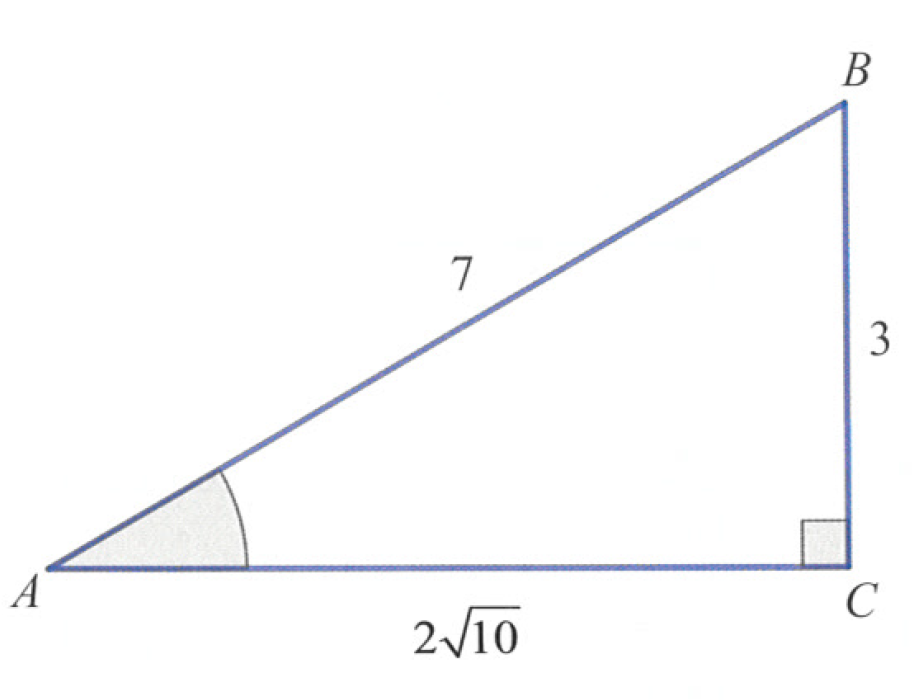
\includegraphics[scale=0.5]{17} 
	\caption{} 
	\label{Figure17} 
\end{figure}
\newpage

\begin{examplebox}
	ให้มุม $A$ เป็นมุมแหลม และ $\tan A = x$ โดยที่ $x \neq 0$ จงหาค่าของฟังก์ชันตรีโกณมิติต่าง ๆ ที่เหลือของมุม $A$
\end{examplebox}
\solution 
\begin{figure}[H] 
	\centering 
	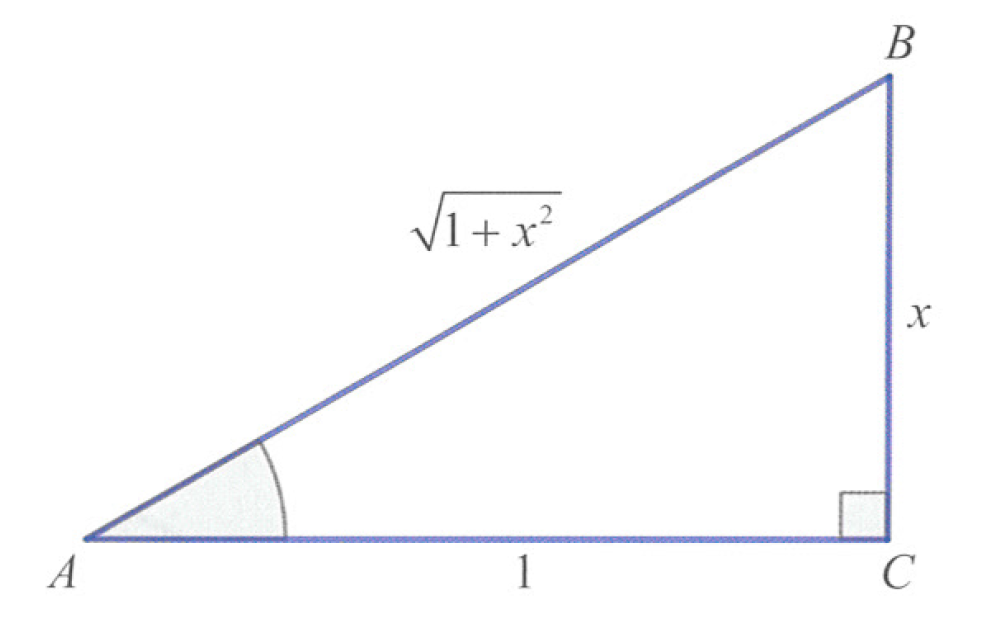
\includegraphics[scale=0.5]{18} 
	\caption{รูปสามเหลี่ยมมุมฉากสำหรับหาอัตราส่วนตรีโกณมิติในรูปของตัวแปร $x$} 
	\label{Figure18} 
\end{figure}
\newpage

\section{กราฟของฟังก์ชันตรีโกณมิติ}
กราฟของฟังก์ชันตรีโกณมิติ โดยเฉพาะกราฟของฟังก์ชันไซน์และโคไซน์เป็นกราฟที่มีความสำคัญ มากทั้งในวิชาคณิตศาสตร์และวิชาอื่น ๆ เช่น ในวิชาฟิสิกส์เรื่องกลศาสตร์ คลื่นแสง คลื่นเสียง คลื่นแม่เหล็กไฟฟ้า ดังนั้น จึงควรศึกษาลักษณะและการเขียนกราฟของฟังก์ชันทั้งสองและฟังก์ชัน อื่น ๆ ที่เกี่ยวข้องดังนี้

การเขียนกราฟของ $y=\sin x$ เขียนได้ดังนี้

กำหนดค่า $x$ และหาค่า $y$ จาก $y=\sin x$ เมื่อ $0 \leq x \leq \pi$ ได้ดังตาราง

\begin{figure}[H] 
	\centering 
	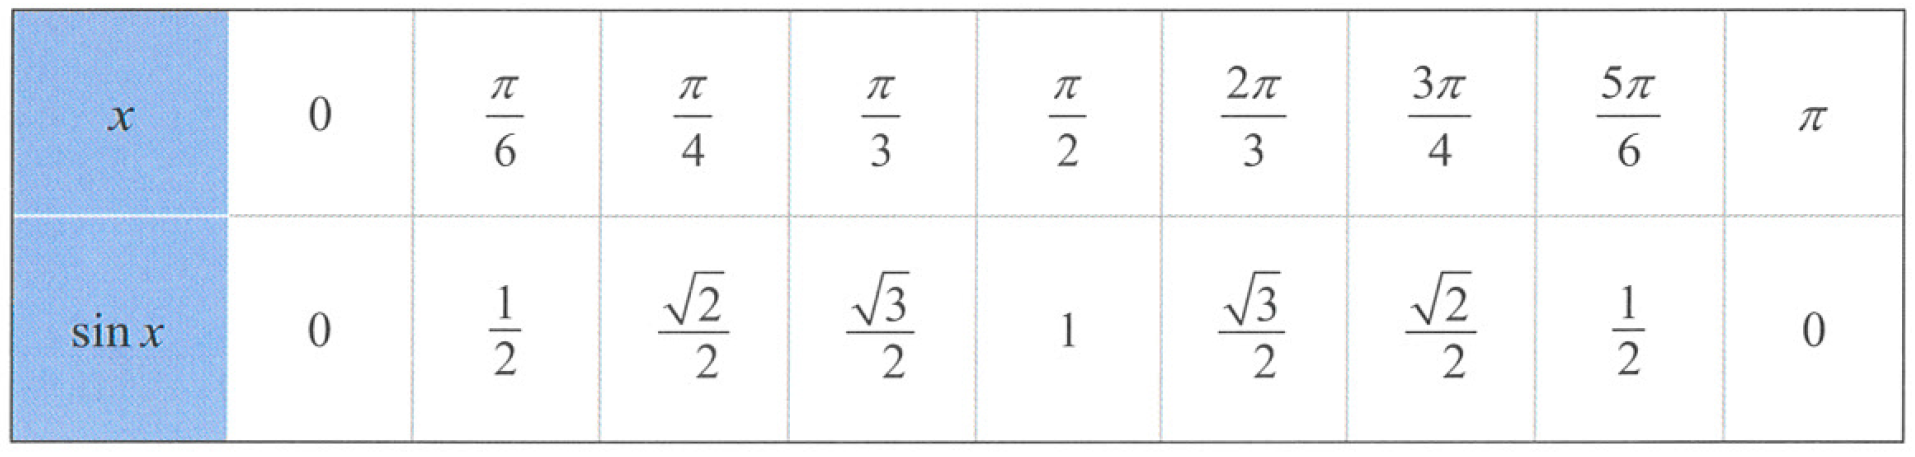
\includegraphics[scale=0.5]{19} 
	\caption{} 
	\label{Figure19} 
\end{figure}

จะได้ กราฟของ $y=\sin x$ เมื่อ $0 \leq x \leq \pi$ เป็นดังนี้

\begin{figure}[H] 
	\centering 
	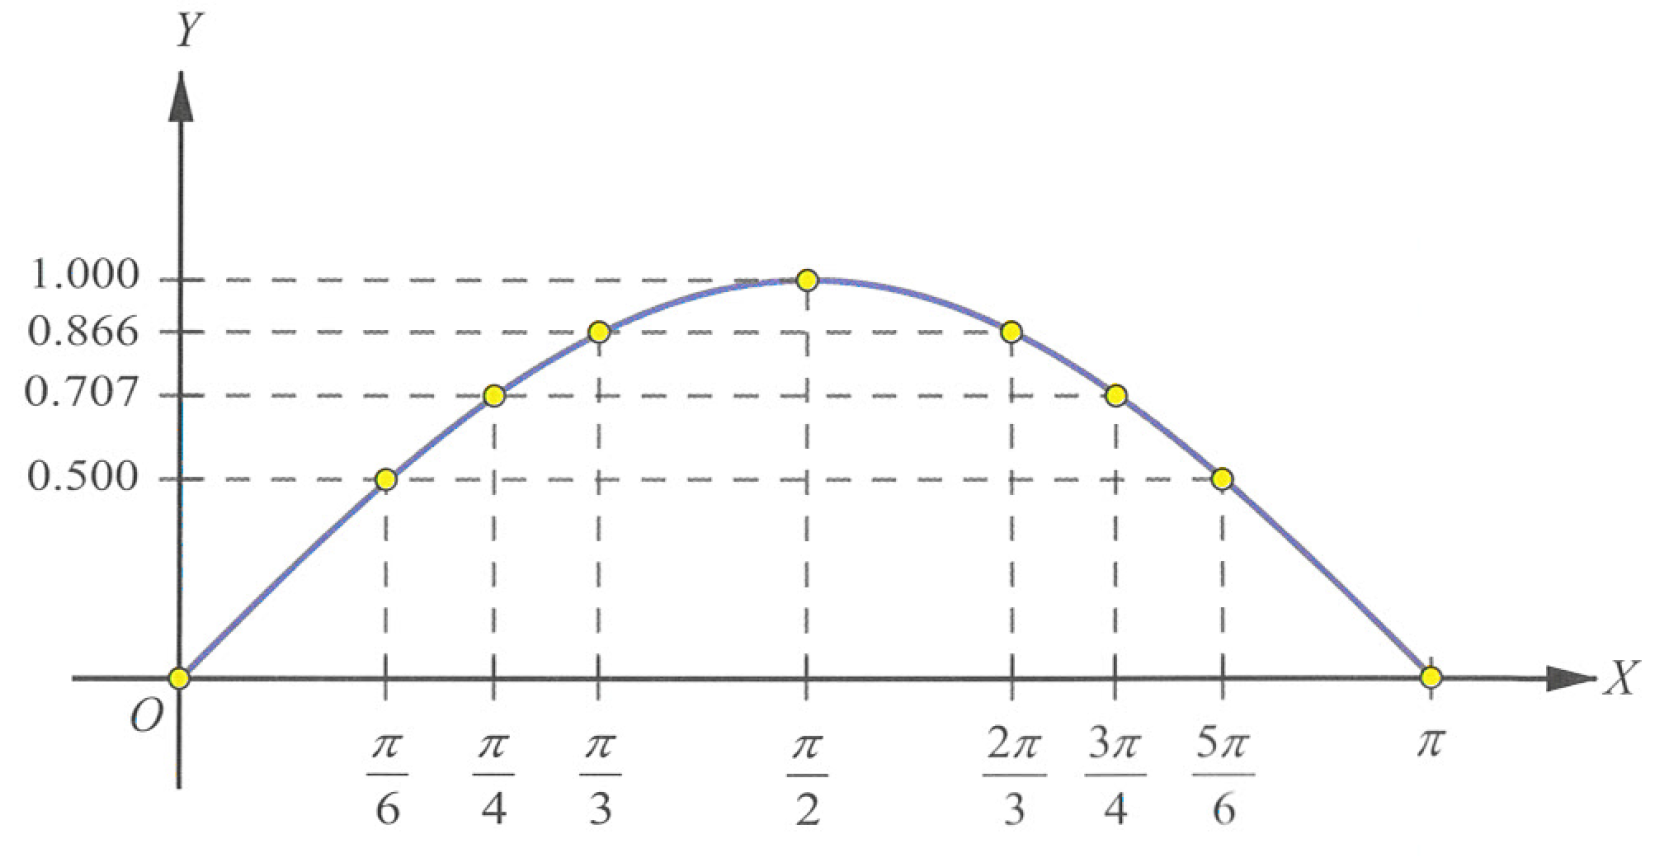
\includegraphics[scale=0.6]{20} 
	\caption{} 
	\label{Figure20} 
\end{figure}

\newpage
เนื่องจากเรนจ์ของฟังก์ชันไซน์ คือ เซตของจำนวนจริงตั้งแต่ $-1$ ถึง $1$ ดังนั้น ค่าของฟังก์ชันไซน์จึง มีค่าตั้งแต่ $-1$ ถึง $1$ ซึ่งค่าของ $\sin x$ เมื่อ $x$ เป็นจำนวนจริงตั้งแต่ $0$ ถึง $2 \pi$ จะมีค่าเพิ่มขึ้นหรือ ลดลงดังแสดงในตารางต่อไปนี้

\begin{figure}[H] 
	\centering 
	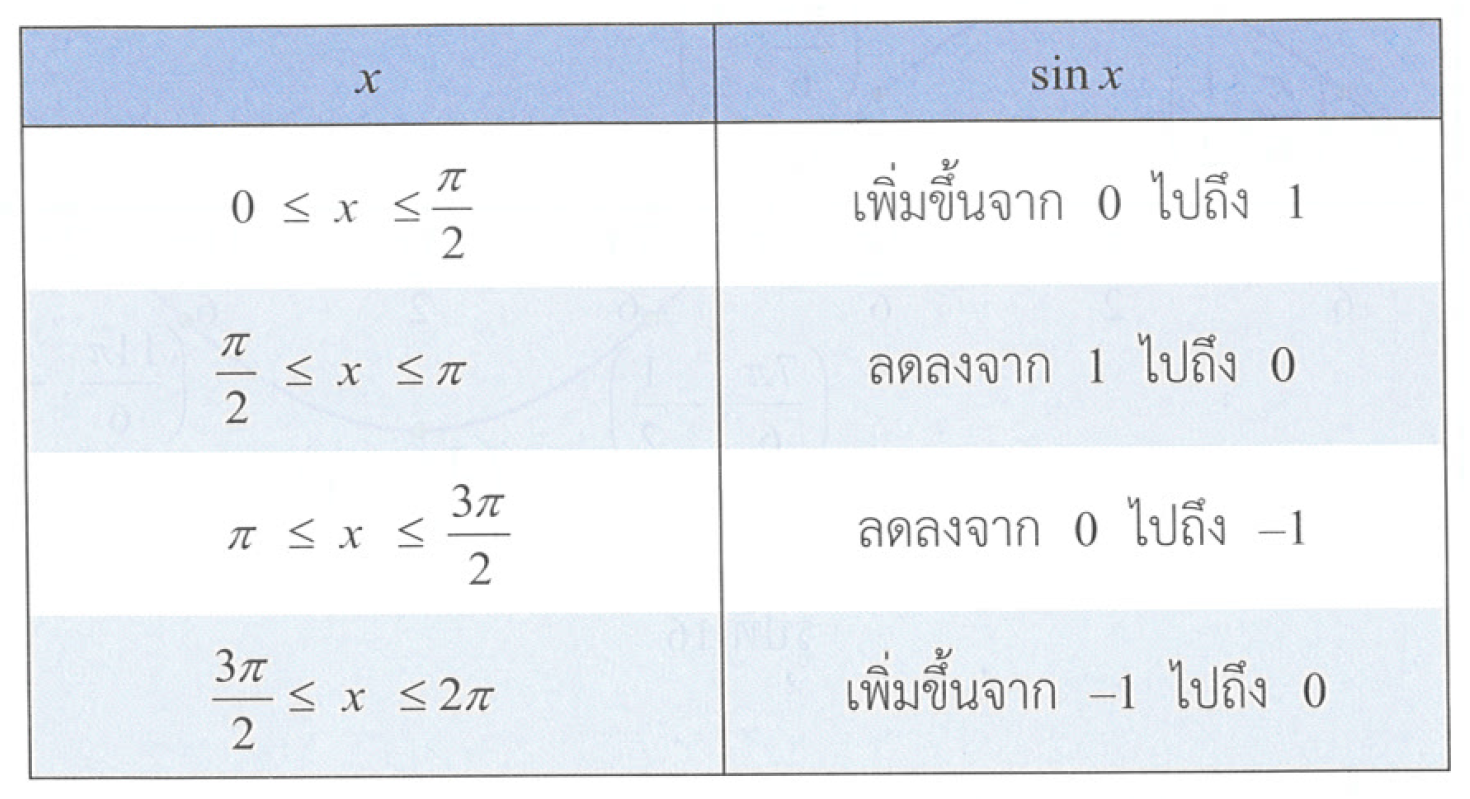
\includegraphics[scale=0.6]{21} 
	\caption{} 
	\label{Figure21} 
\end{figure}

กำหนดค่า $x$ และหาค่า $y$ จาก $y=\sin x$ เมื่อ $0 \leq x \leq 2 \pi$ ได้ดังตาราง

\begin{figure}[H] 
	\centering 
	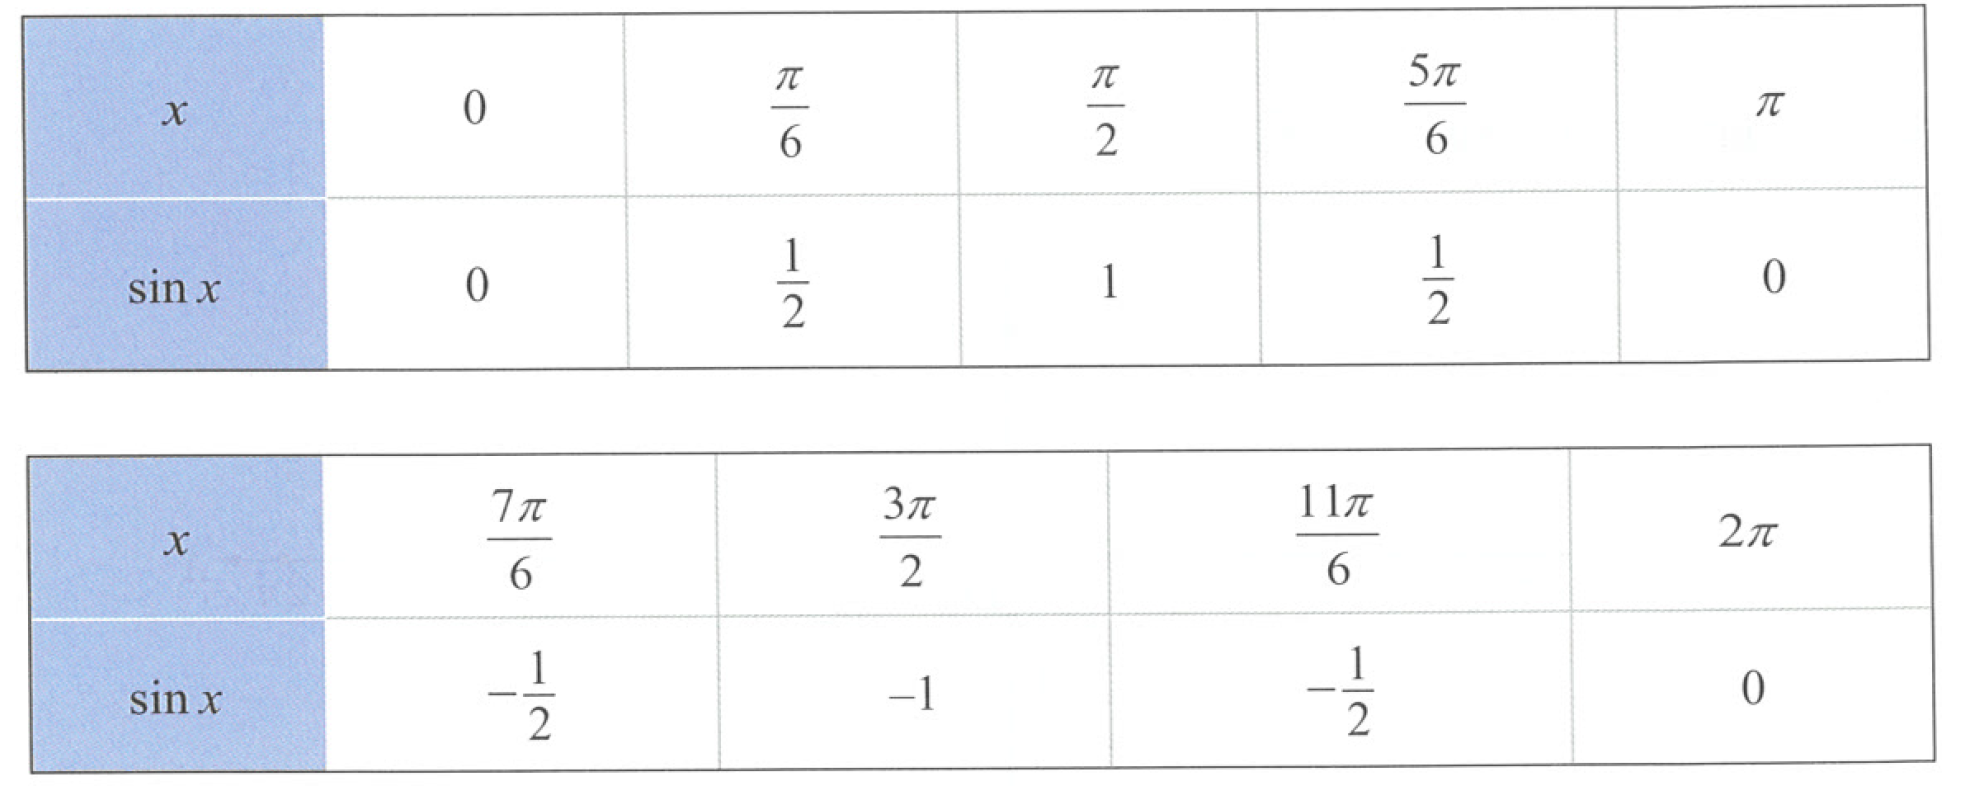
\includegraphics[scale=0.5]{22} 
	\caption{} 
	\label{Figure22} 
\end{figure}

\newpage
จะได้ กราฟของ $y=\sin x$ เมื่อ $0 \leq x \leq 2 \pi$ เป็นดังนี้

\begin{figure}[H] 
	\centering 
	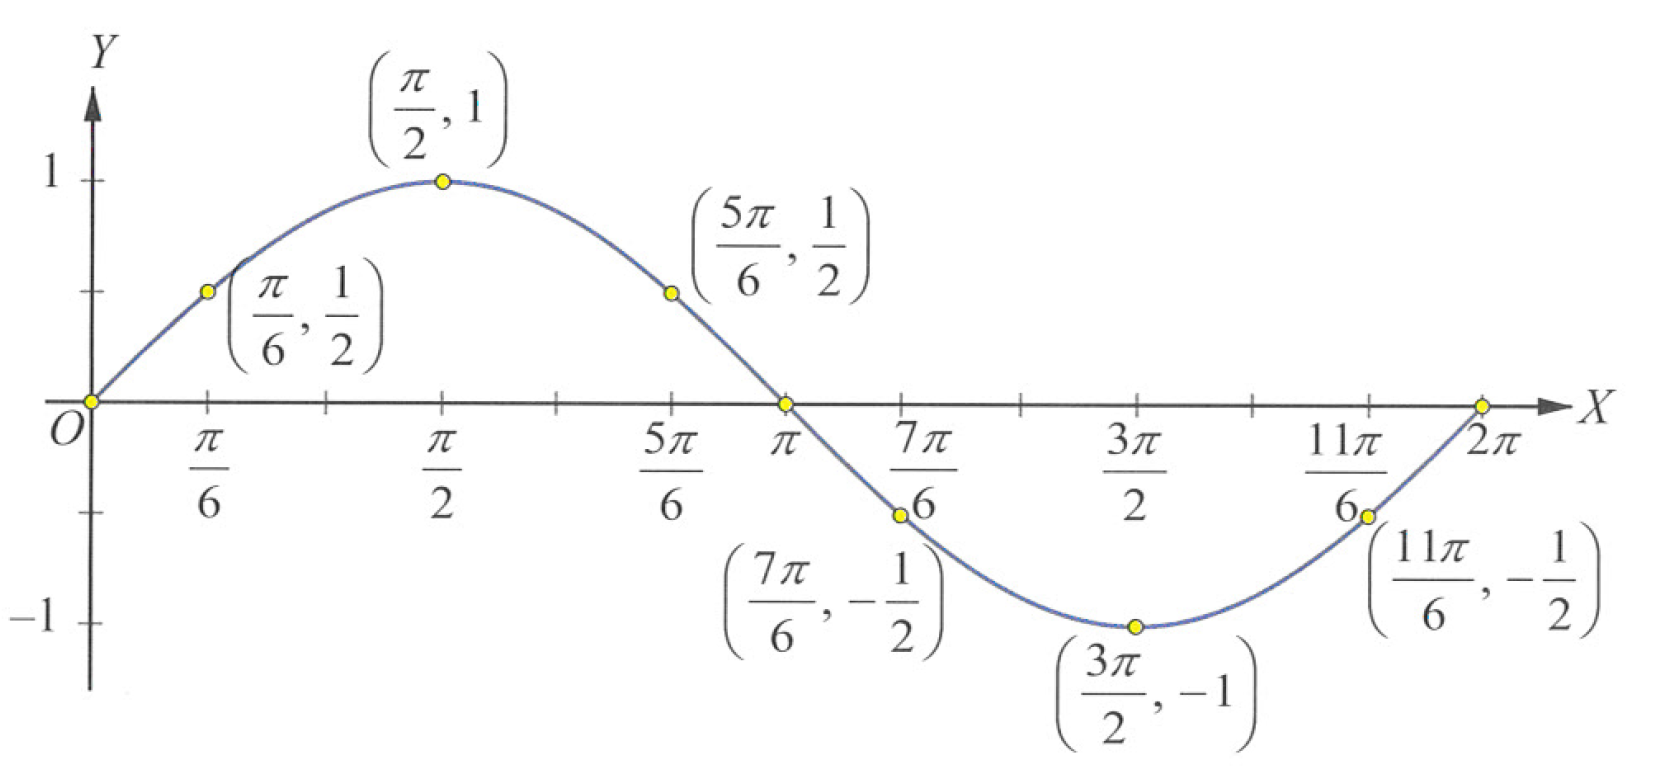
\includegraphics[scale=0.6]{23} 
	\caption{} 
	\label{Figure23} 
\end{figure}

จากที่ทราบมาแล้วว่า $\sin (2 n \pi+x)=\sin x$ เมื่อ $n$ เป็นจำนวนเต็ม สมบัตินี้เป็นสมบัติที่สำคัญ อย่างหนึ่งของฟังก์ชันไซน์ ทำให้กราฟของฟังก์ชันไซน์มีลักษณะซ้ำกันเป็นช่วง ๆ ซึ่งช่วยให้การเขียน กราฟง่ายขึ้น

จะได้ กราฟของ $y=\sin x$ เป็นดังนี้

\begin{figure}[H] 
	\centering 
	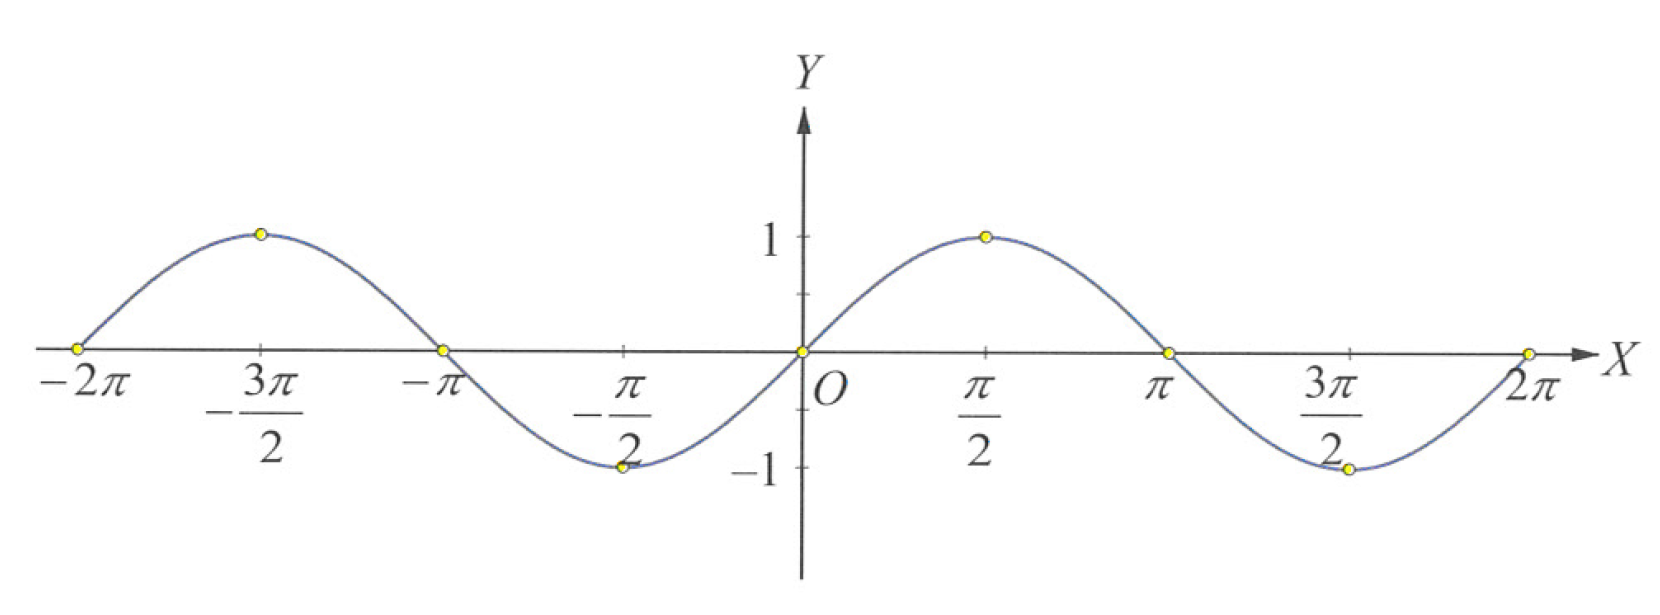
\includegraphics[scale=0.6]{24} 
	\caption{} 
	\label{Figure24} 
\end{figure}

จากกราฟ จะเห็นว่า โดเมนของฟังก์ชันไซน์ คือ เซตของจำนวนจริง
\\
เรนจ์ของฟังก์ชันไซน์ คือ $[-1,1]$
\\
กราฟของฟังก์ชันไซน์ตัดแกน $X$ ที่จุด $(x, 0)$ เมื่อ $x$ คือ $\ldots,-2 \pi,-\pi, 0, \pi, 2 \pi, \ldots$
\\
กราฟของฟังก์ชันไซน์ตัดแกน $Y$ ที่จุด $(0,0)$

\vspace{0.5em}
\noindent ในทำนองเดียวกันกับการเขียนกราฟของ $y=\sin x$ จะเขียนกราฟของ $y=\cos x$ ได้ดังนี้

\vspace{0.5em}
\noindent กำหนดค่า $x$ และหาค่า $y$ จาก $y=\cos x$ ได้ดังตาราง

\begin{figure}[H] 
	\centering 
	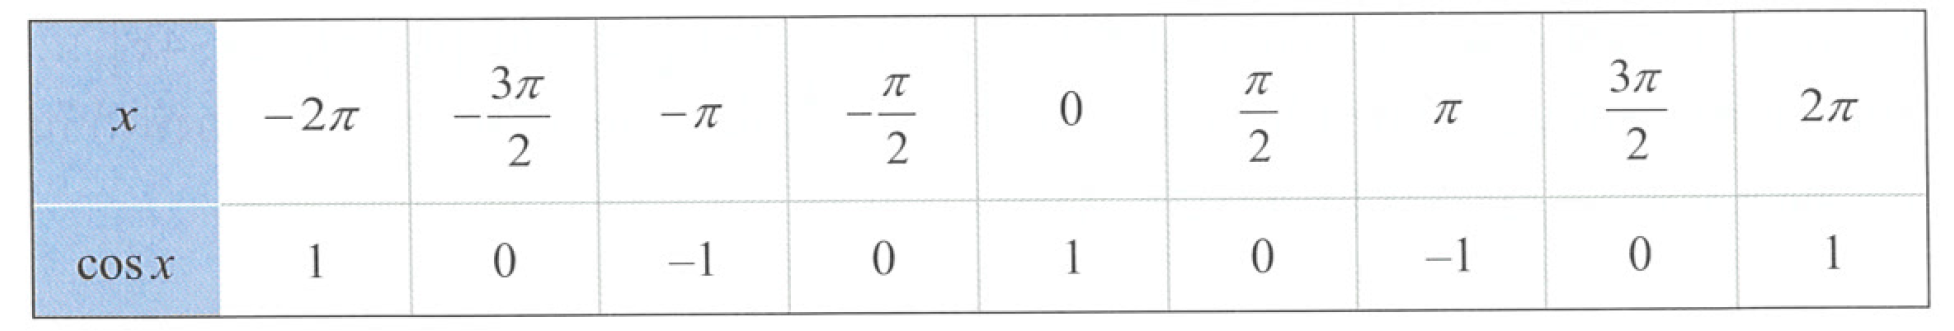
\includegraphics[scale=0.6]{25} 
	\caption{} 
	\label{Figure25} 
\end{figure}

จะได้ กราฟของ $y=\cos x$ เป็นดังนี้

\begin{figure}[H] 
	\centering 
	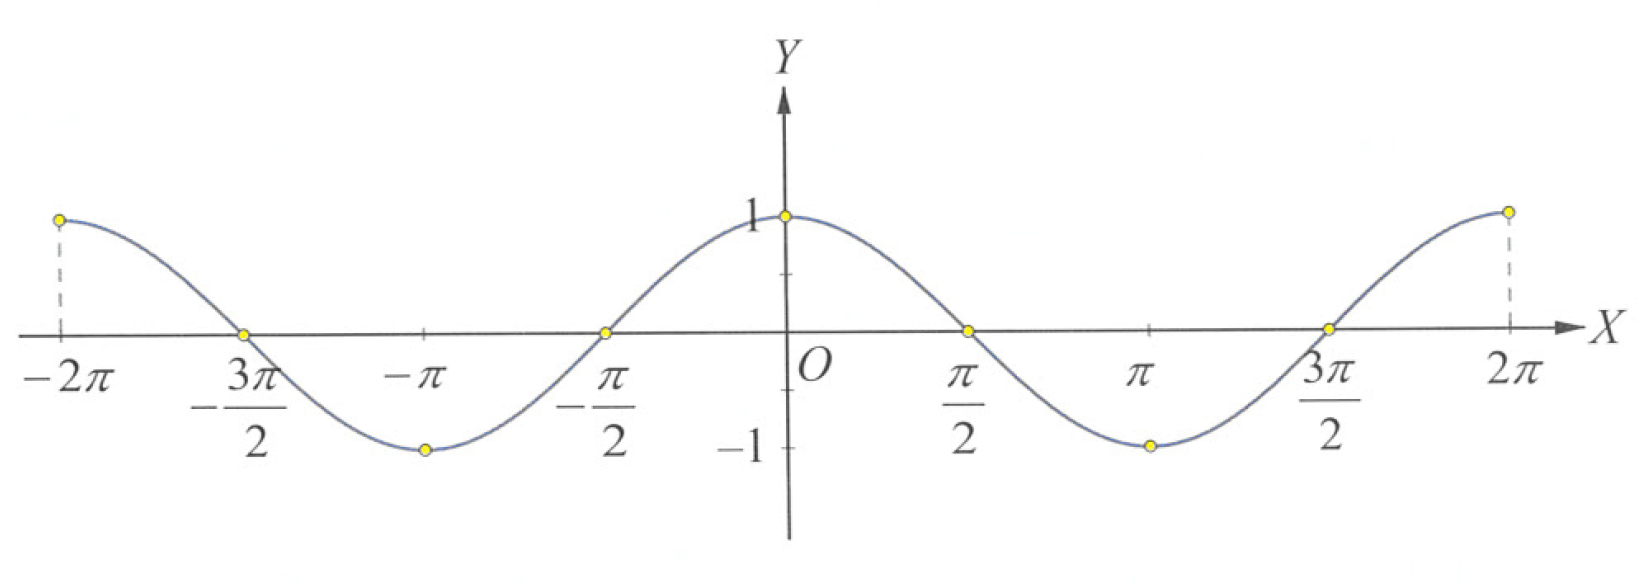
\includegraphics[scale=0.6]{26} 
	\caption{} 
	\label{Figure26} 
\end{figure}

\vspace{0.5em}
\noindent จากกราฟ จะเห็นว่า โดเมนของฟังก์ชันโคไซน์ คือ เซตของจำนวนจริง เรนจ์ของฟังก์ชันโคไซน์ คือ $[-1,1]$
\\
กราฟของฟังก์ชันโคไซน์ตัดแกน $X$ ที่จุด $(x, 0)$ เมื่อ $x$ คือ $\ldots,-\dfrac{3 \pi}{2},-\dfrac{\pi}{2}, \dfrac{\pi}{2}, \dfrac{3 \pi}{2}, \ldots$ กราฟของฟังก์ชันโคไซน์ตัดแกน $Y$ ที่จุด $(0,1)$

ฟังก์ชันตรีโกณมิติเป็น \textbf{ฟังก์ชันที่เป็นคาบ (periodic function)} กล่าวคือ สามารถแบ่งแกน $X$ ออกเป็น \textbf{ช่วงย่อย (subinterval)} โดยที่ความยาวของแต่ละช่วงย่อยเท่ากันและกราฟในแต่ละช่วงย่อยมีลักษณะ เหมือนกัน ความยาวของช่วงย่อยที่สั้นที่สุดที่มีสมบัติดังกล่าวเรียกว่า \textbf{คาบ (period)} ของฟังก์ชัน เช่น กราฟของ $y=\sin x$ และ $y=\cos x$ ในช่วง $\ldots,[-4 \pi,-2 \pi],[-2 \pi, 0],[0,2 \pi],[2 \pi, 4 \pi], \ldots$ เป็นช่วงที่สั้นที่สุดที่แบ่งแล้วทำให้กราฟในแต่ละช่วงเหล่านั้นมีลักษณะเหมือนกัน คาบของฟังก์ชัน $y=\sin x$ และ $y=\cos x$ จึงเท่ากับ $2 \pi$ ดังรูป

\begin{figure}[H] 
	\centering 
	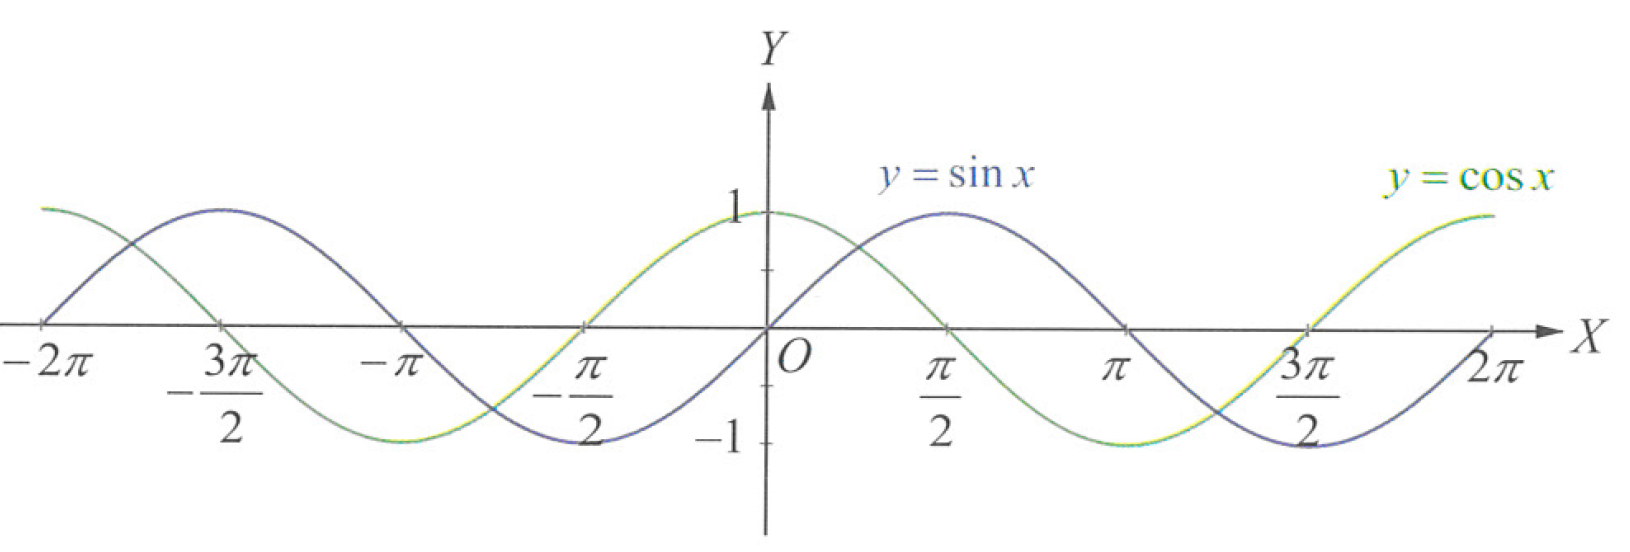
\includegraphics[scale=0.6]{27} 
	\caption{} 
	\label{Figure27} 
\end{figure}

สำหรับฟังก์ชันที่เป็นคาบซึ่งมีค่าสูงสุดและค่าต่ำสุด จะเรียกค่าที่เท่ากับครึ่งหนึ่งของผลต่างระหว่าง ค่าสูงสุดและค่าต่ำสุดของฟังก์ชันนั้นว่า \textbf{แอมพลิจูด (amplitude)}
\\
นั่นคือ ถ้า $a$ เป็นค่าสูงสุด และ $b$ เป็นค่าต่ำสุดของฟังก์ชันที่เป็นคาบ แล้วจะได้ว่าแอมพลิจูดของ ฟังก์ชันนี้ คือ $\dfrac{1}{2}(a-b)$
\\
ดังนั้น ฟังก์ชัน $y=\sin x$ และ $y=\cos x$ มีแอมพลิจูดเป็น $1$ เท่ากัน

\newpage
\begin{examplebox}
	จงเขียนกราฟของ $y=\sin x$ และ $y=2 \sin x$ ในระบบพิกัดฉากเดียวกัน พร้อมทั้งหาจุดตัดแกน $X$ โดเมน เรนจ์ คาบ และแอมพลิจูดของฟังก์ชัน $y=2 \sin x$
\end{examplebox}
\solution 
กำหนดค่า $x$ และหาค่า $y$ จาก $y=\sin x$ และ $y=2 \sin x$ ได้ดังตาราง
\begin{figure}[H] 
	\centering 
	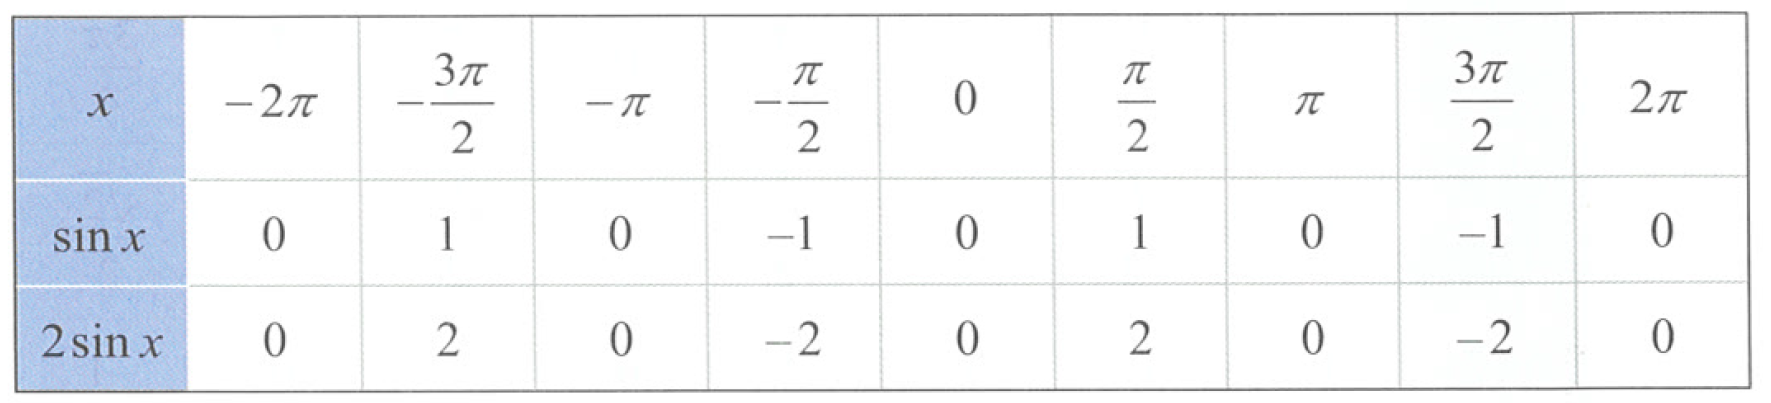
\includegraphics[scale=0.6]{28} 
	\caption{} 
	\label{Figure28} 
\end{figure}
จากตารางสามารถเขียนกราฟได้ดังนี้
\begin{figure}[H] 
	\centering 
	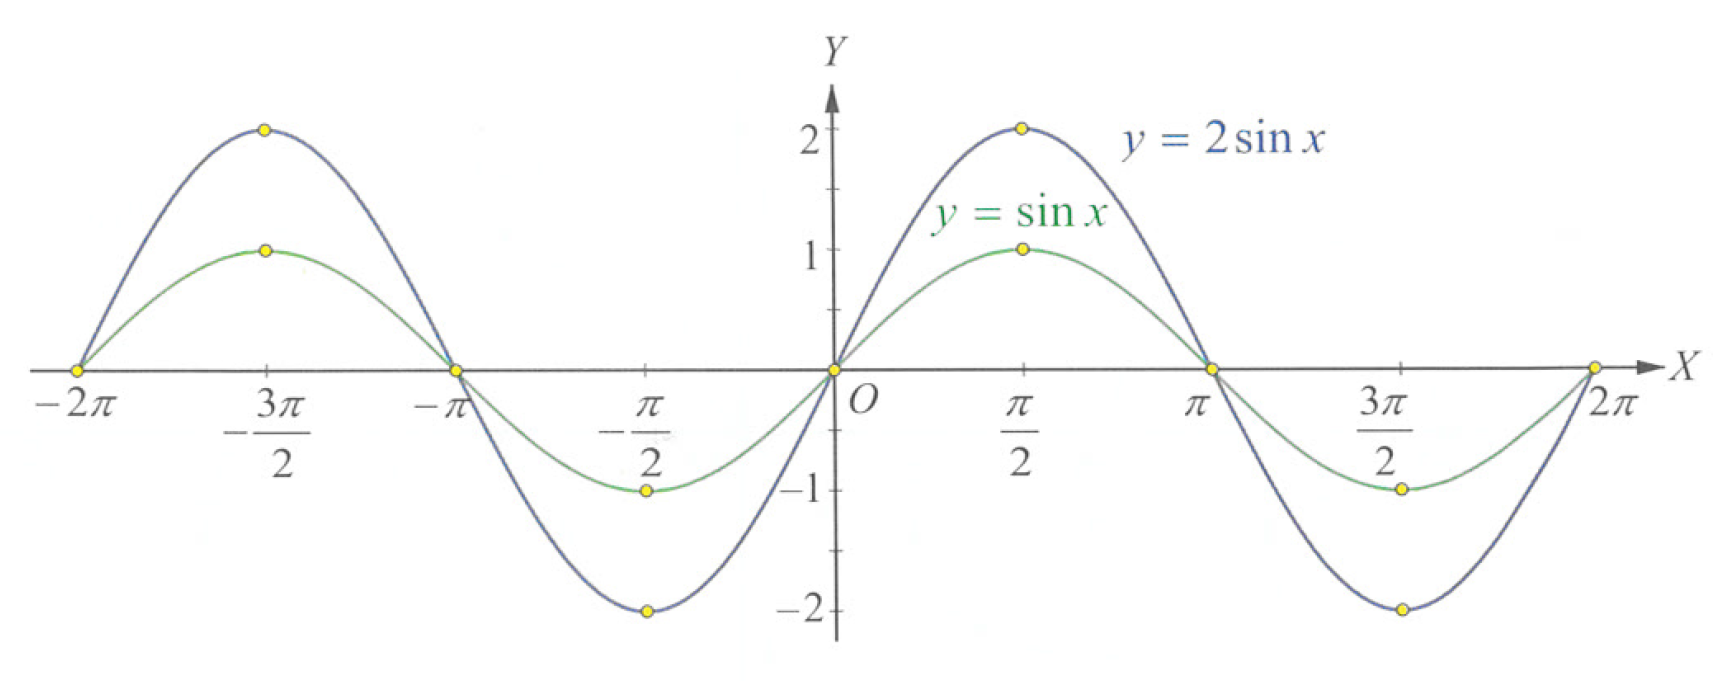
\includegraphics[scale=0.6]{29} 
	\caption{} 
	\label{Figure29} 
\end{figure}
จากกราฟ จะเห็นว่า กราฟของ $y=\sin x$ และ $y=2 \sin x$ ตัดแกน $X$ ที่จุดเดียวกัน คือ จุด $(x, 0)$ เมื่อ $x$ คือ $\ldots,-2 \pi,-\pi, 0, \pi, 2 \pi, \ldots$
\\
โดเมนของฟังก์ชัน $y=2 \sin x$ คือ เซตของจำนวนจริง
\\
เรนจ์ของฟังก์ชัน $y=2 \sin x$ คือ $[-2,2]$
\\
คาบของฟังก์ชัน $y=2 \sin x$ คือ $2 \pi$
\\
และแอมพลิจูดของฟังก์ชัน $y=2 \sin x$ คือ $\dfrac{2-(-2)}{2}=2$
\newpage
\begin{examplebox}
	จงเขียนกราฟของ $y=\sin x$ และ $y=\sin 2 x$ ในระบบพิกัดฉากเดียวกัน พร้อมทั้งหาจุดตัดแกน $X$ โดเมน เรนจ์ คาบ และแอมพลิจูดของฟังก์ชัน $y=\sin 2 x$
\end{examplebox}
\solution 
กำหนดค่า $x$ และหาค่า $y$ จาก $y=\sin x$ และ $y=\sin 2 x$ ได้ดังตาราง
\begin{figure}[H] 
	\centering 
	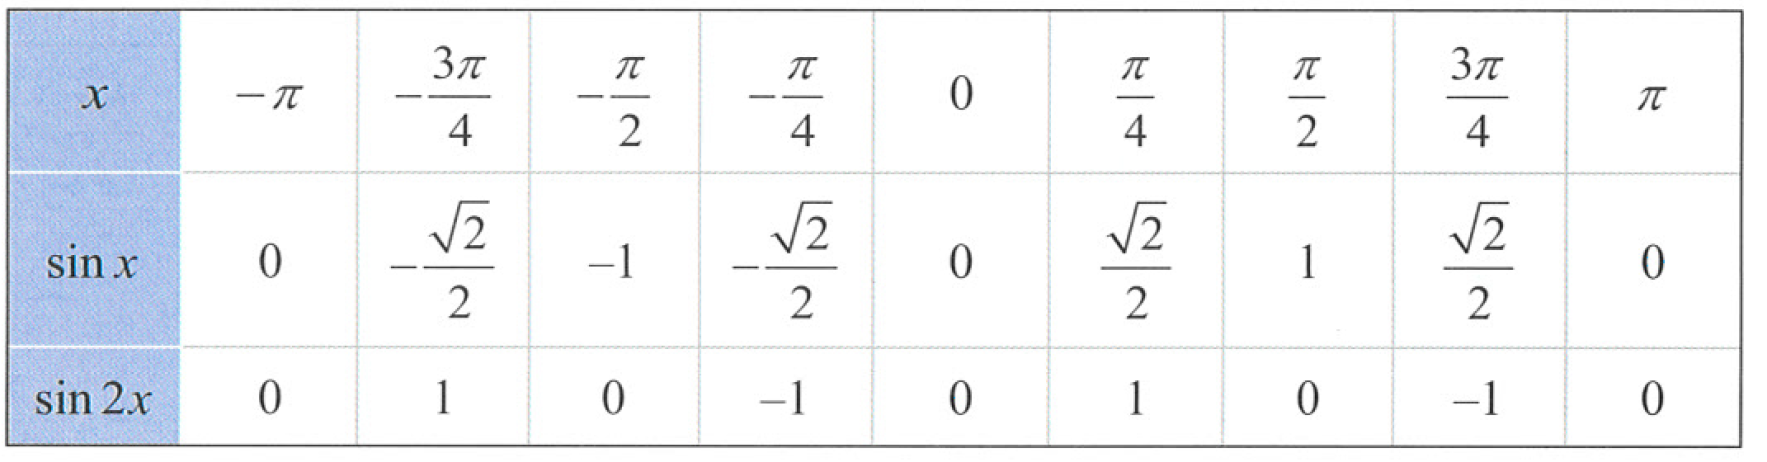
\includegraphics[scale=0.6]{30} 
	\caption{} 
	\label{Figure30} 
\end{figure}
จากตารางสามารถเขียนกราฟได้ดังนี้
\begin{figure}[H] 
	\centering 
	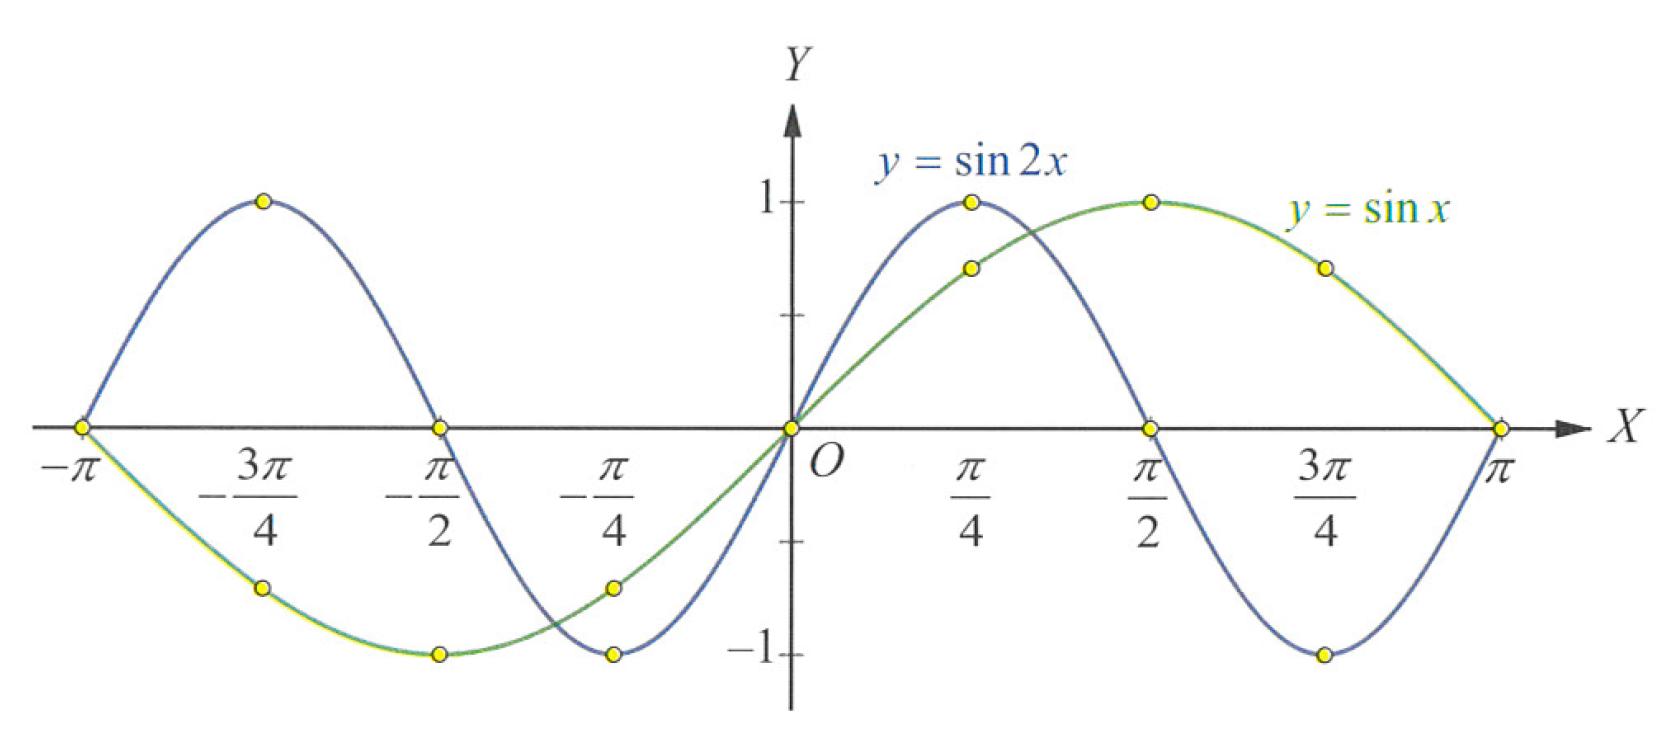
\includegraphics[scale=0.6]{31} 
	\caption{} 
	\label{Figure31} 
\end{figure}
จากกราฟ จะเห็นว่า กราฟของ $y=\sin 2 x$ ตัดแกน $X$ ที่จุด $(x, 0)$ เมื่อ $x$ คือ $\ldots$, $-2 \pi$, $-\dfrac{3 \pi}{2}$, $-\pi$, $-\dfrac{\pi}{2}$, $0$, $\dfrac{\pi}{2}$, $\pi$, $\dfrac{3 \pi}{2}$, $2 \pi$, $\ldots$
\\
โดเมนของฟังก์ชัน $y=\sin 2 x$ คือ เซตของจำนวนจริง
\\
เรนจ์ของฟังก์ชัน $y=\sin 2 x$ คือ $[-1,1]$
\\
คาบของฟังก์ชัน $y=\sin 2 x$ คือ $\pi$
\\
และแอมพลิจูดของฟังก์ชัน $y=\sin 2 x$ คือ $\dfrac{1-(-1)}{2}=1$

\newpage
\begin{examplebox}
	จงเขียนกราฟของ $y=\sin x$ และ $y=\sin \dfrac{x}{2}$ ในระบบพิกัดฉากเดียวกัน พร้อมทั้งหาจุดตัดแกน $X$ โดเมน เรนจ์ คาบ และแอมพลิจูดของฟังก์ชัน $y=\sin \dfrac{x}{2}$
\end{examplebox}
\solution 
กำหนดค่า $x$ และหาค่า $y$ จาก $y=\sin x$ และ $y=\sin \dfrac{x}{2}$ ได้ดังตาราง
\begin{figure}[H] 
	\centering 
	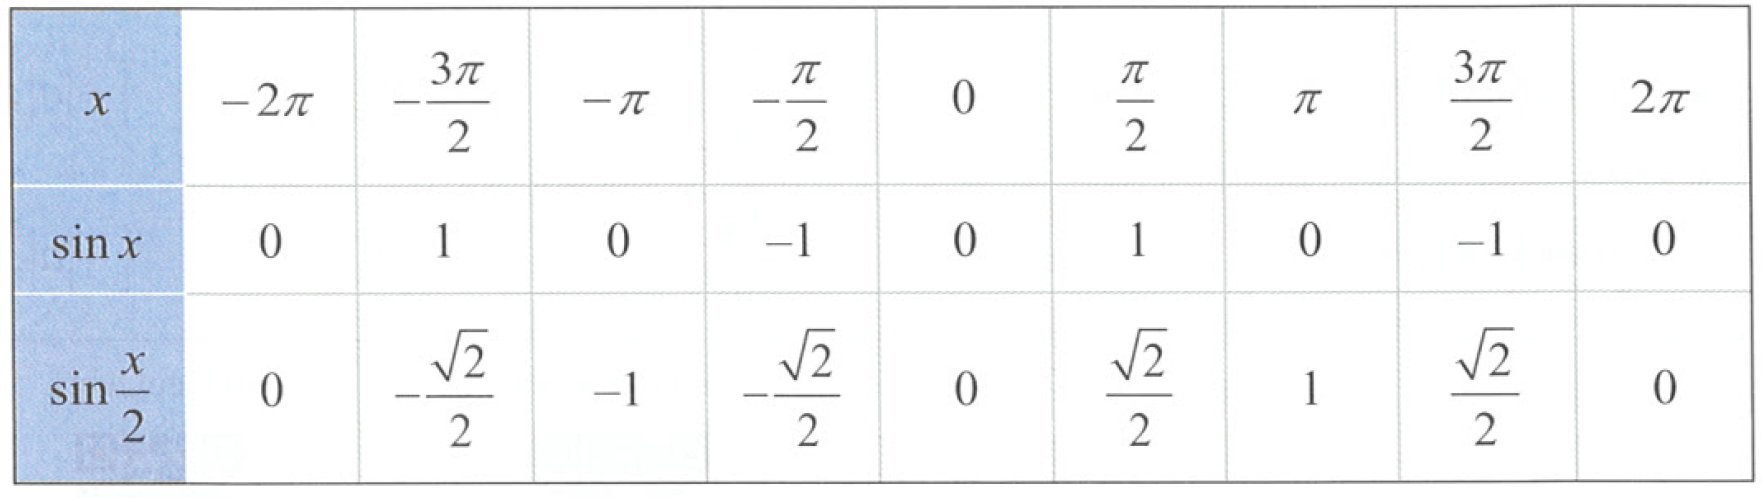
\includegraphics[scale=0.6]{32} 
	\caption{} 
	\label{Figure32} 
\end{figure}
จากตารางสามารถเขียนกราฟได้ดังนี้
\begin{figure}[H] 
	\centering 
	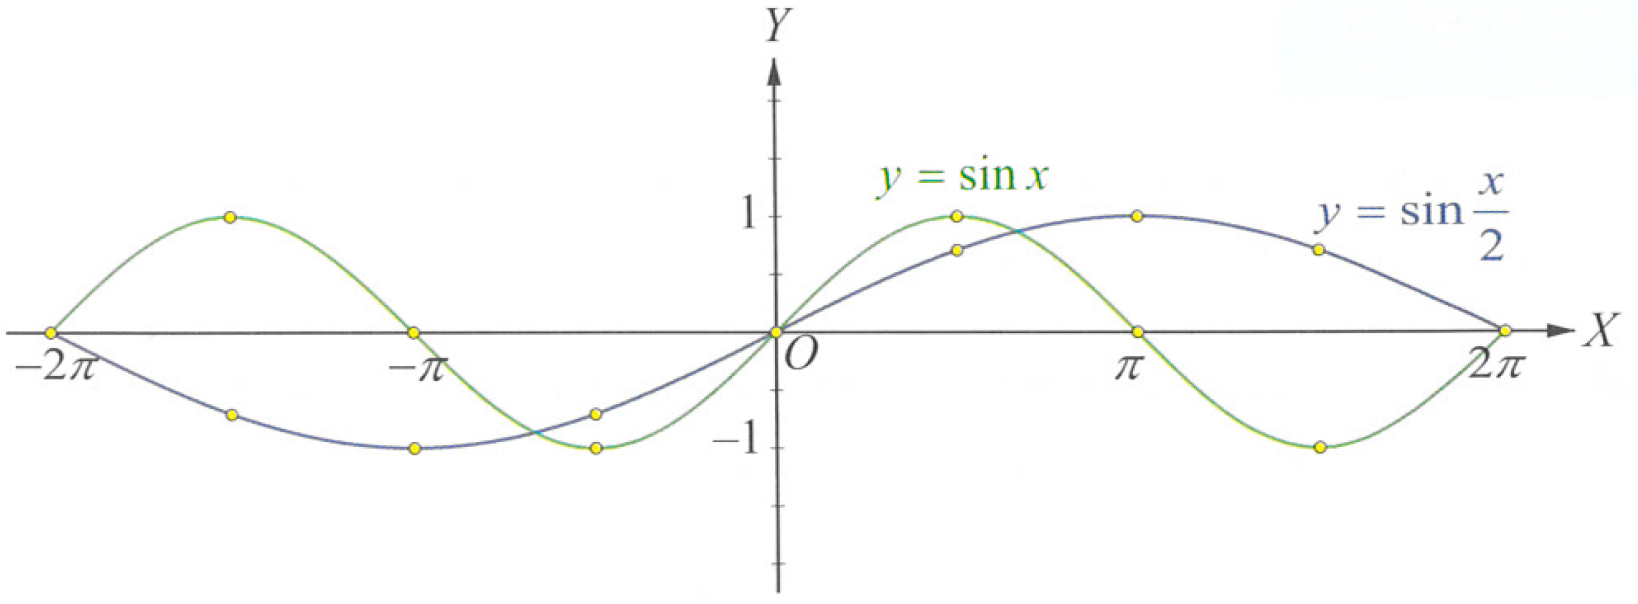
\includegraphics[scale=0.6]{33} 
	\caption{} 
	\label{Figure33} 
\end{figure}
จากกราฟ จะเห็นว่า กราฟของ $y=\sin \dfrac{x}{2}$ ตัดแกน $X$ ที่จุด $(x, 0)$ เมื่อ $x$ คือ $\ldots$, $-4 \pi$, $-2 \pi$, $0$, $2 \pi$, $4 \pi$, $\ldots$
\\
โดเมนของฟังก์ชัน $y=\sin \dfrac{x}{2}$ คือ เซตของจำนวนจริง
\\
เรนจ์ของฟังก์ชัน $y=\sin \dfrac{x}{2}$ คือ $[-1,1]$
\\
คาบของฟังก์ชัน $y=\sin \dfrac{x}{2}$ คือ $4 \pi$
\\
และแอมพลิจูดของฟังก์ชัน $y=\sin \dfrac{x}{2}$ คือ $\dfrac{1-(-1)}{2}=1$

\newpage
ในกรณีทั่วไป จะได้ว่า
\begin{figure}[H] 
	\centering 
	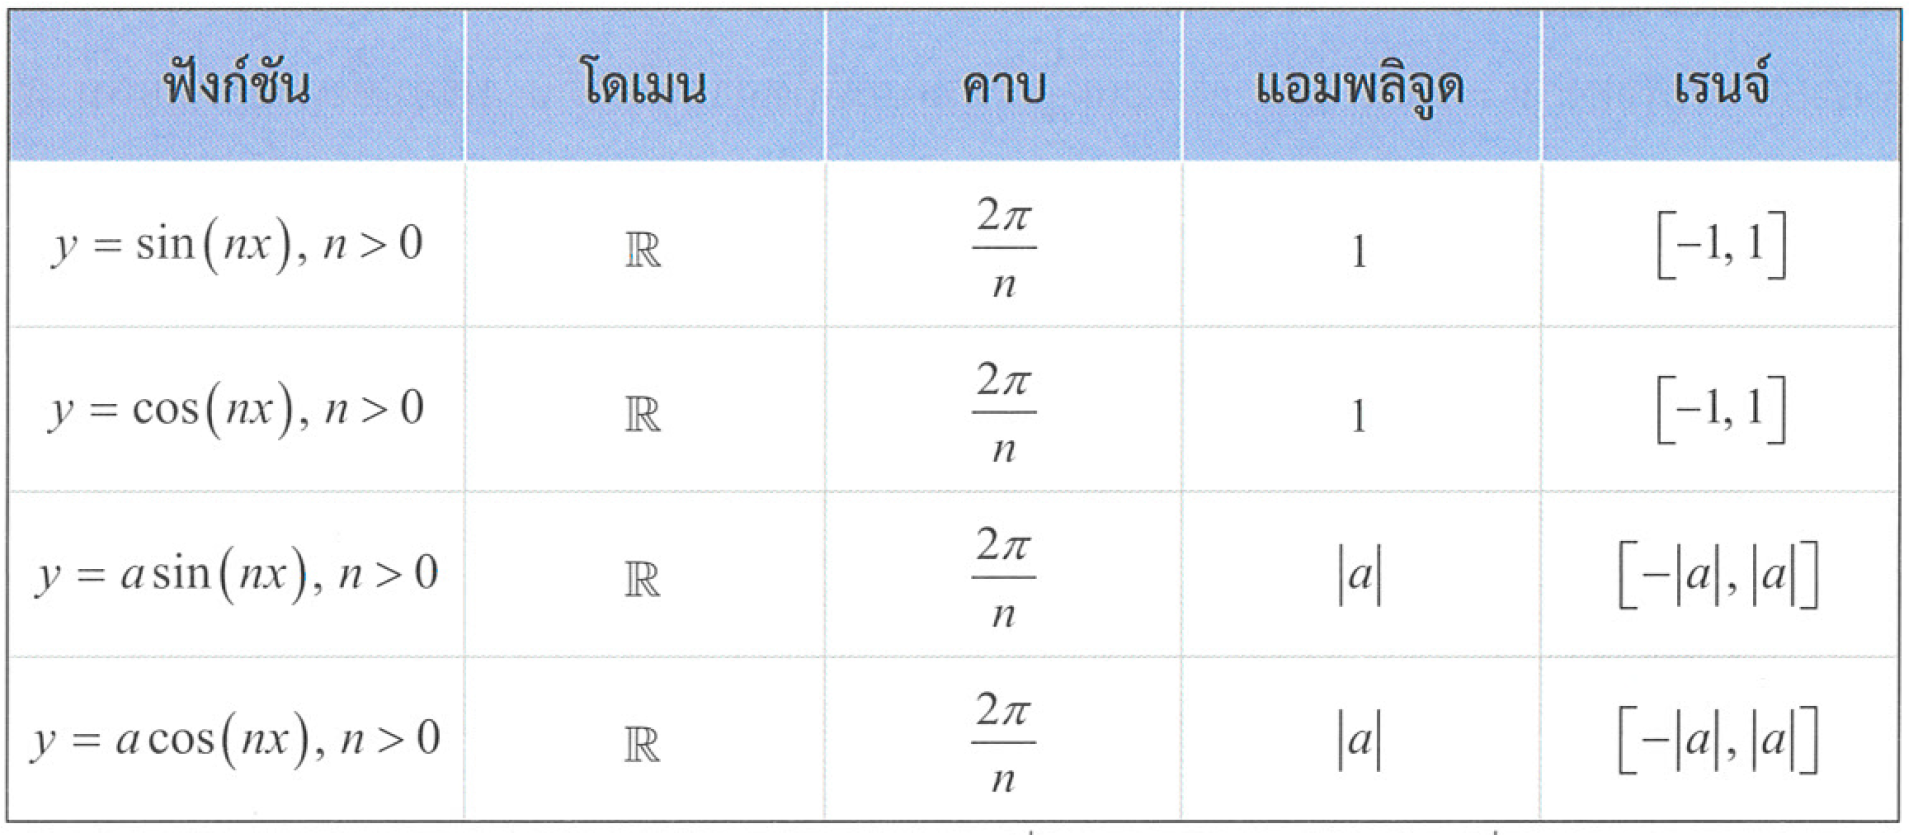
\includegraphics[scale=0.55]{34} 
	\caption{} 
	\label{Figure34} 
\end{figure}

\begin{examplebox}
	จงหาคาบ แอมพลิจูด และเรนจ์ของฟังก์ชัน $y=3 \cos x$ พร้อมทั้งเขียนกราฟของ $y=\cos x$ และ $y=3 \cos x$ ในระบบพิกัดฉากเดียวกัน
\end{examplebox}
\solution จาก $y=3 \cos x$ จะได้ คาบ คือ $2 \pi$ แอมพลิจูด คือ $3$ และเรนจ์ คือ $[-3,3]$ เขียนกราฟของ $y=\cos x$ และ $y=3 \cos x$ ได้ดังนี้
\begin{figure}[H] 
	\centering 
	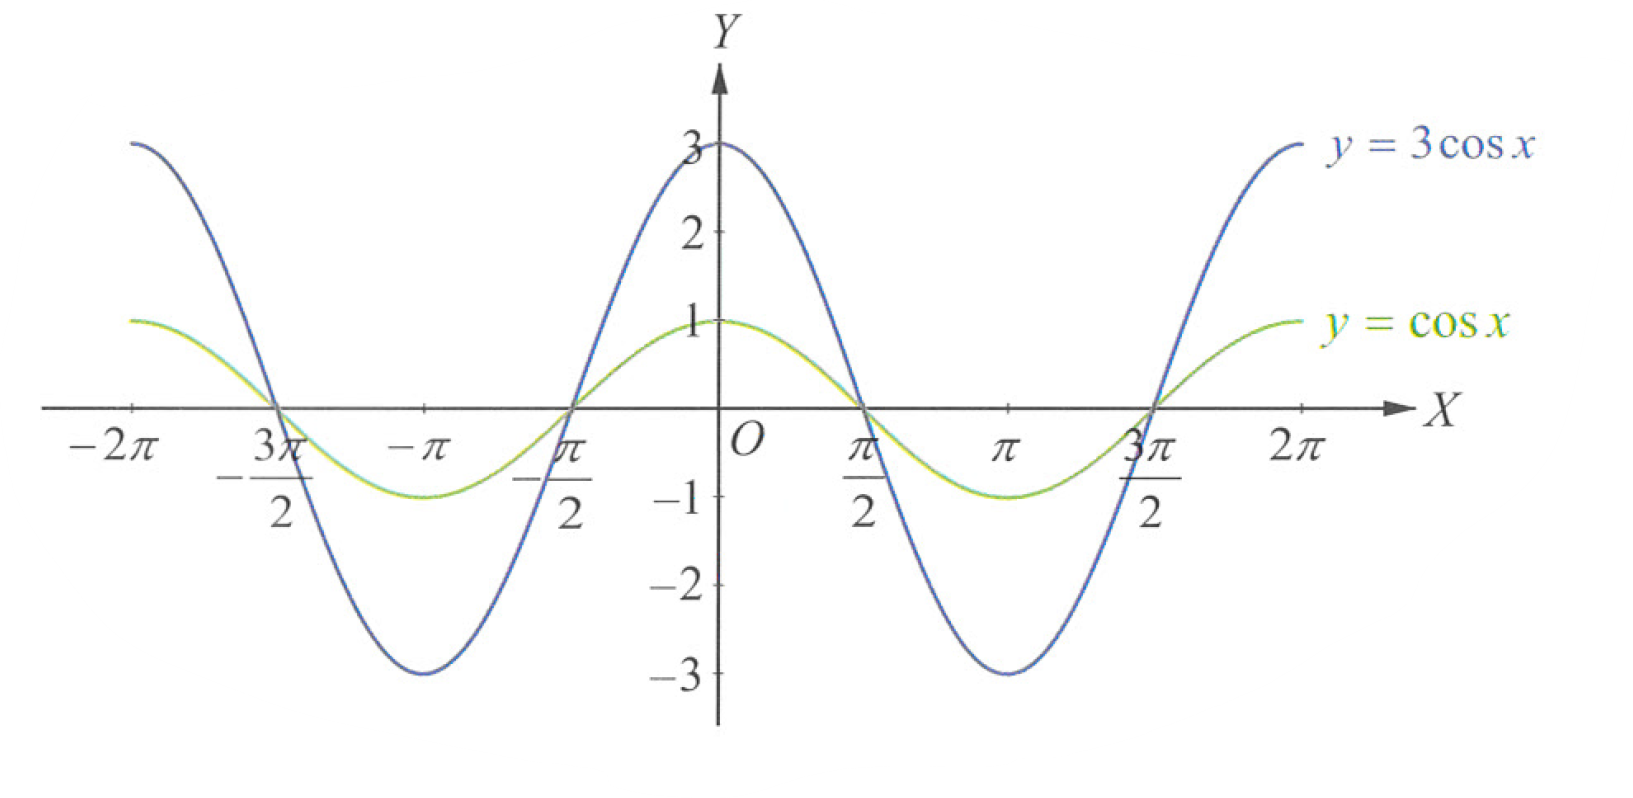
\includegraphics[scale=0.6]{35} 
	\caption{} 
	\label{Figure35} 
\end{figure}
\observation จากตัวอย่างข้างต้นกราฟของ $y=\cos x$ และ $y=3 \cos x$ ตัดแกน $X$ ที่จุดเดียวกัน
\newpage
\begin{examplebox}
	จงหาคาบ แอมพลิจูด และเรนจ์ของฟังก์ชัน $y=3 \sin 2 x$ พร้อมทั้งเขียนกราฟ
\end{examplebox}
\solution จาก $y=3 \sin 2 x$ จะได้ คาบ คือ $\dfrac{2 \pi}{2}=\pi$ แอมพลิจูด คือ $3$ และเรนจ์ คือ $[-3,3]$ เขียนกราฟของ $y=3 \sin 2 x$ ได้ดังนี้
\begin{figure}[H] 
	\centering 
	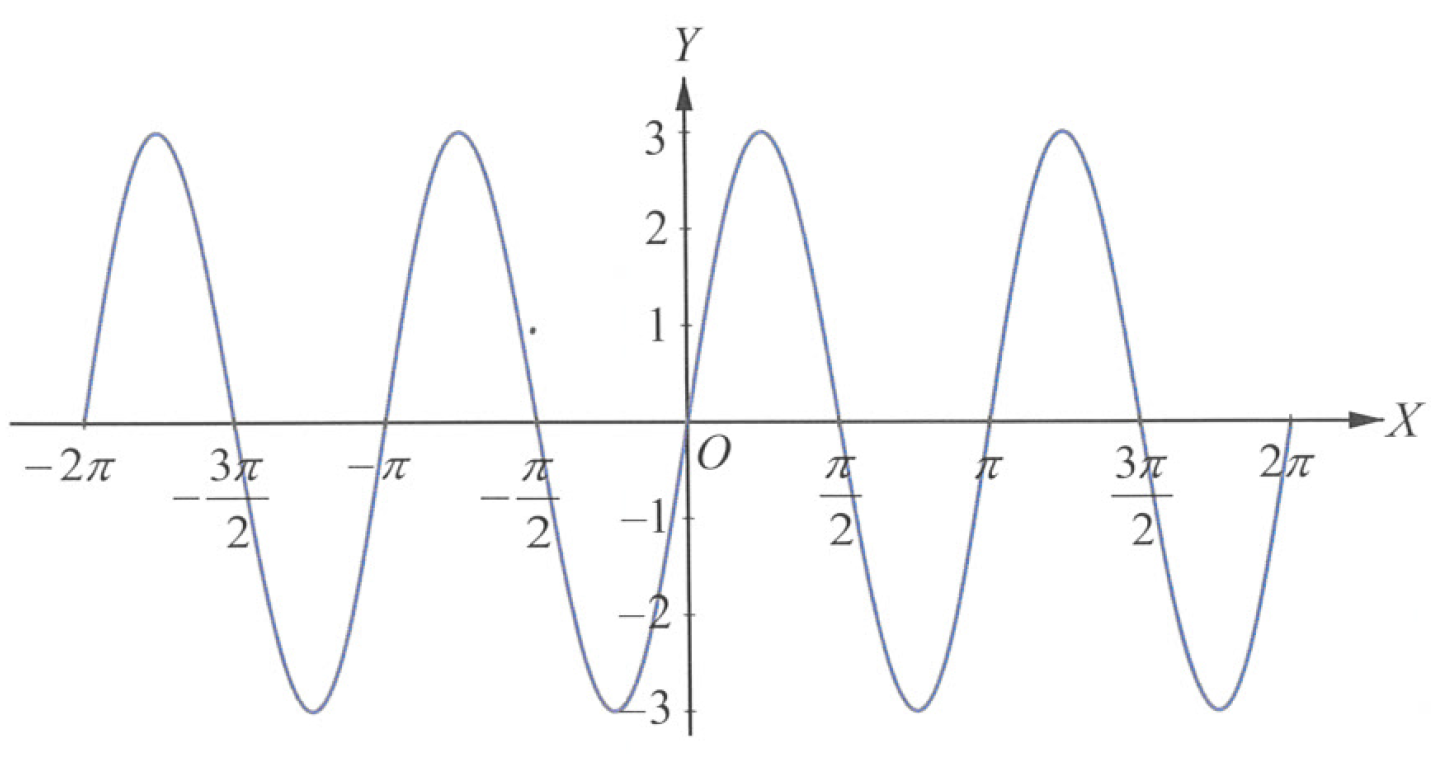
\includegraphics[scale=0.6]{36} 
	\caption{} 
	\label{Figure36} 
\end{figure}

\newpage
ก่อนจะเขียนกราฟของฟังก์ชันตรีโกณมิติอื่น ๆ ให้พิจารณาโดเมนของฟังก์ชันตรีโกณมิติต่อไปนี้

\noindent โดเมนของฟังก์ชันไซน์และโคไซน์ คือ $\mathbb{R}$
\\
โดเมนของฟังก์ชันแทนเจนต์ คือ $\left\{x \left\lvert\, x \neq n \pi+\dfrac{\pi}{2}\right., n \in \mathbb{Z}\right\}$
\\
โดเมนของฟังก์ชันเซแคนต์ คือ $\left\{x \left\lvert\, x \neq n \pi+\dfrac{\pi}{2}\right., n \in \mathbb{Z}\right\}$
\\
โดเมนของฟังก์ชันโคแทนเจนต์ คือ $\{x \mid x \neq n \pi, n \in \mathbb{Z}\}$
\\
โดเมนของฟังก์ชันโคเซแคนต์ คือ $\{x \mid x \neq n \pi, n \in \mathbb{Z}\}$

\vspace{0.5em}
\noindent การเขียนกราฟของ $y=\tan x$ เขียนได้ดังนี้
\\
กำหนดค่า $x$ และหาค่า $y$ จาก $y=\tan x$ เมื่อ $-\dfrac{\pi}{2}<x<\dfrac{\pi}{2}$ ได้ดังตาราง
\begin{figure}[H] 
	\centering 
	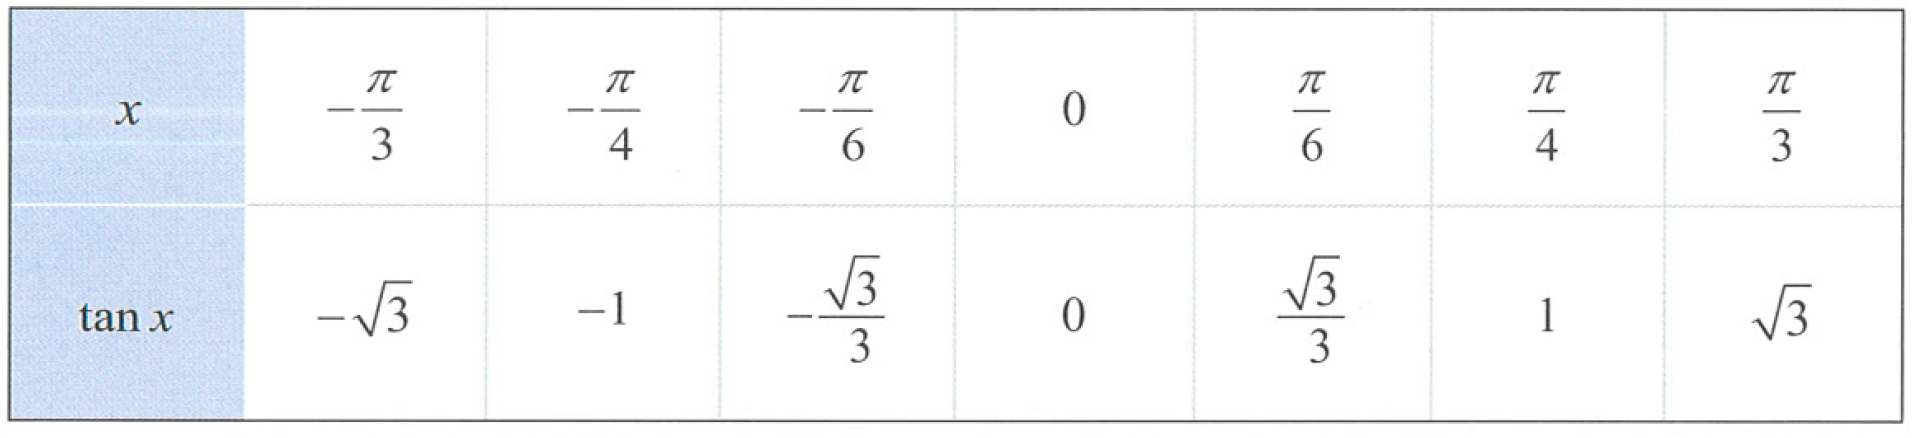
\includegraphics[scale=0.5]{37} 
	\caption{} 
	\label{Figure37} 
\end{figure}
จะได้กราฟของ $y=\tan x$ เมื่อ $-\dfrac{\pi}{2}<x<\dfrac{\pi}{2}$ เป็นดังนี้
\begin{figure}[H] 
	\centering 
	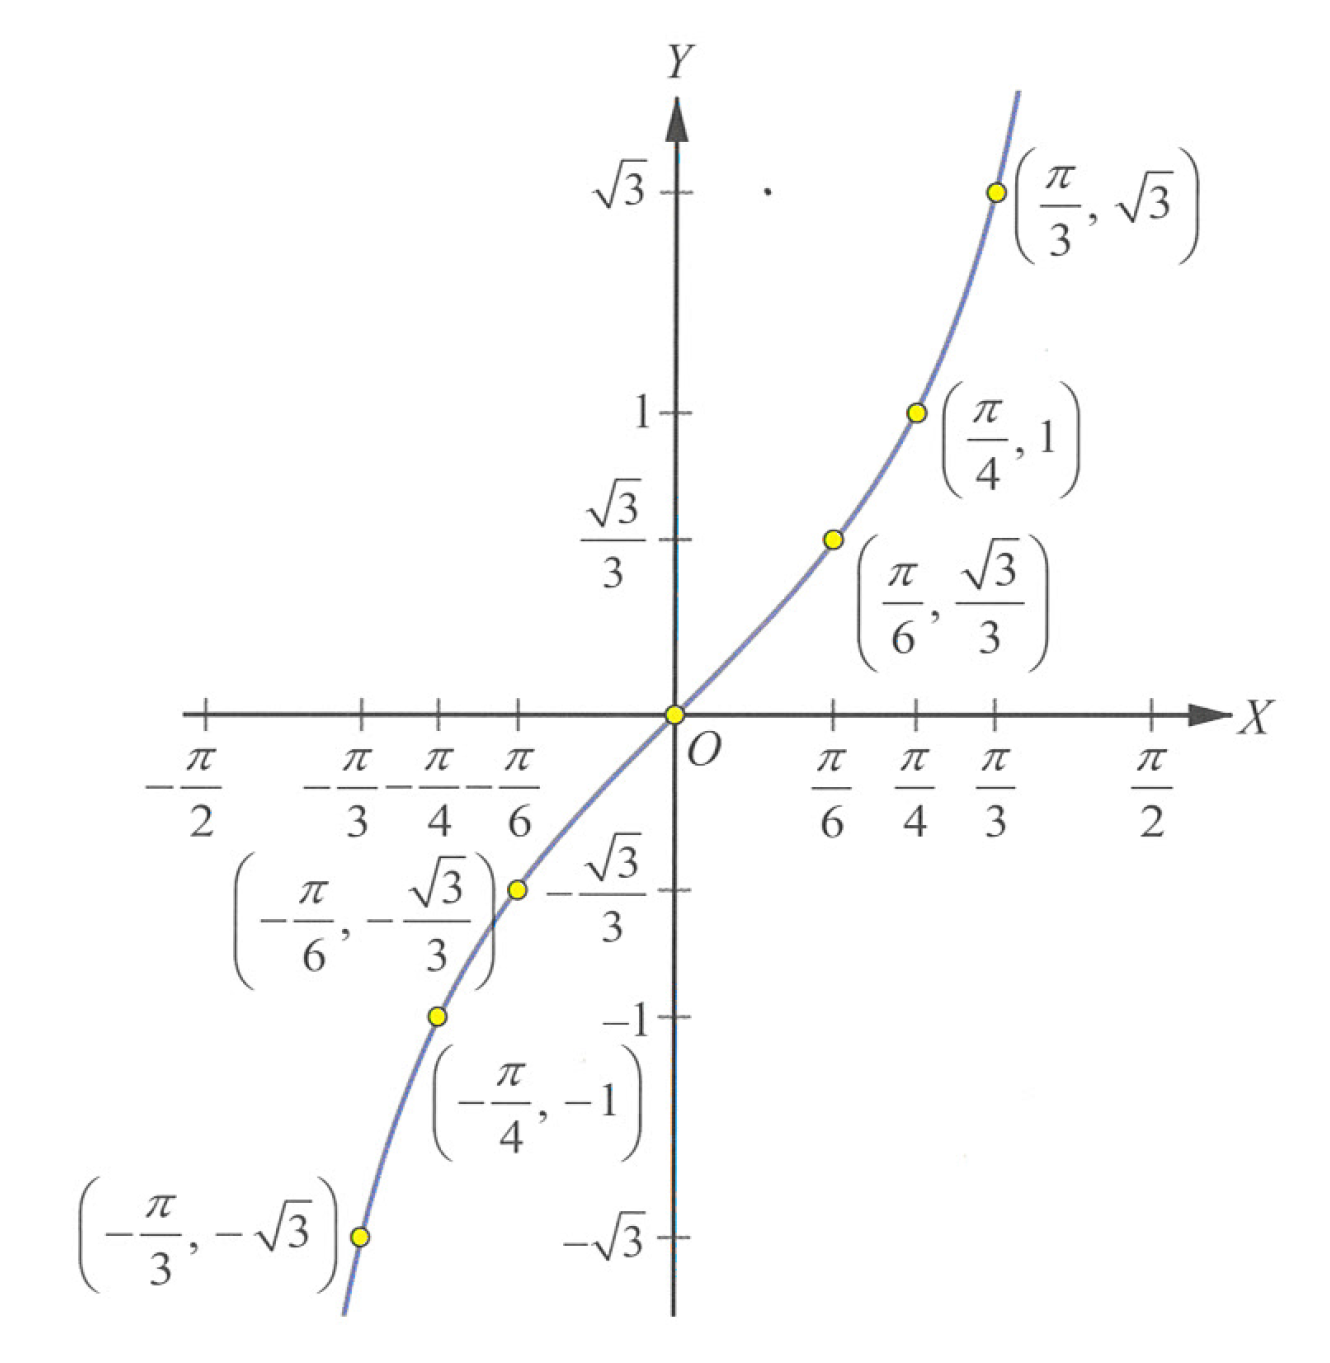
\includegraphics[scale=0.5]{38} 
	\caption{} 
	\label{Figure38} 
\end{figure}

พิจารณากราฟของ $y=\tan x$ เมื่อ $0 \leq x \leq 2 \pi$
\begin{figure}[H] 
	\centering 
	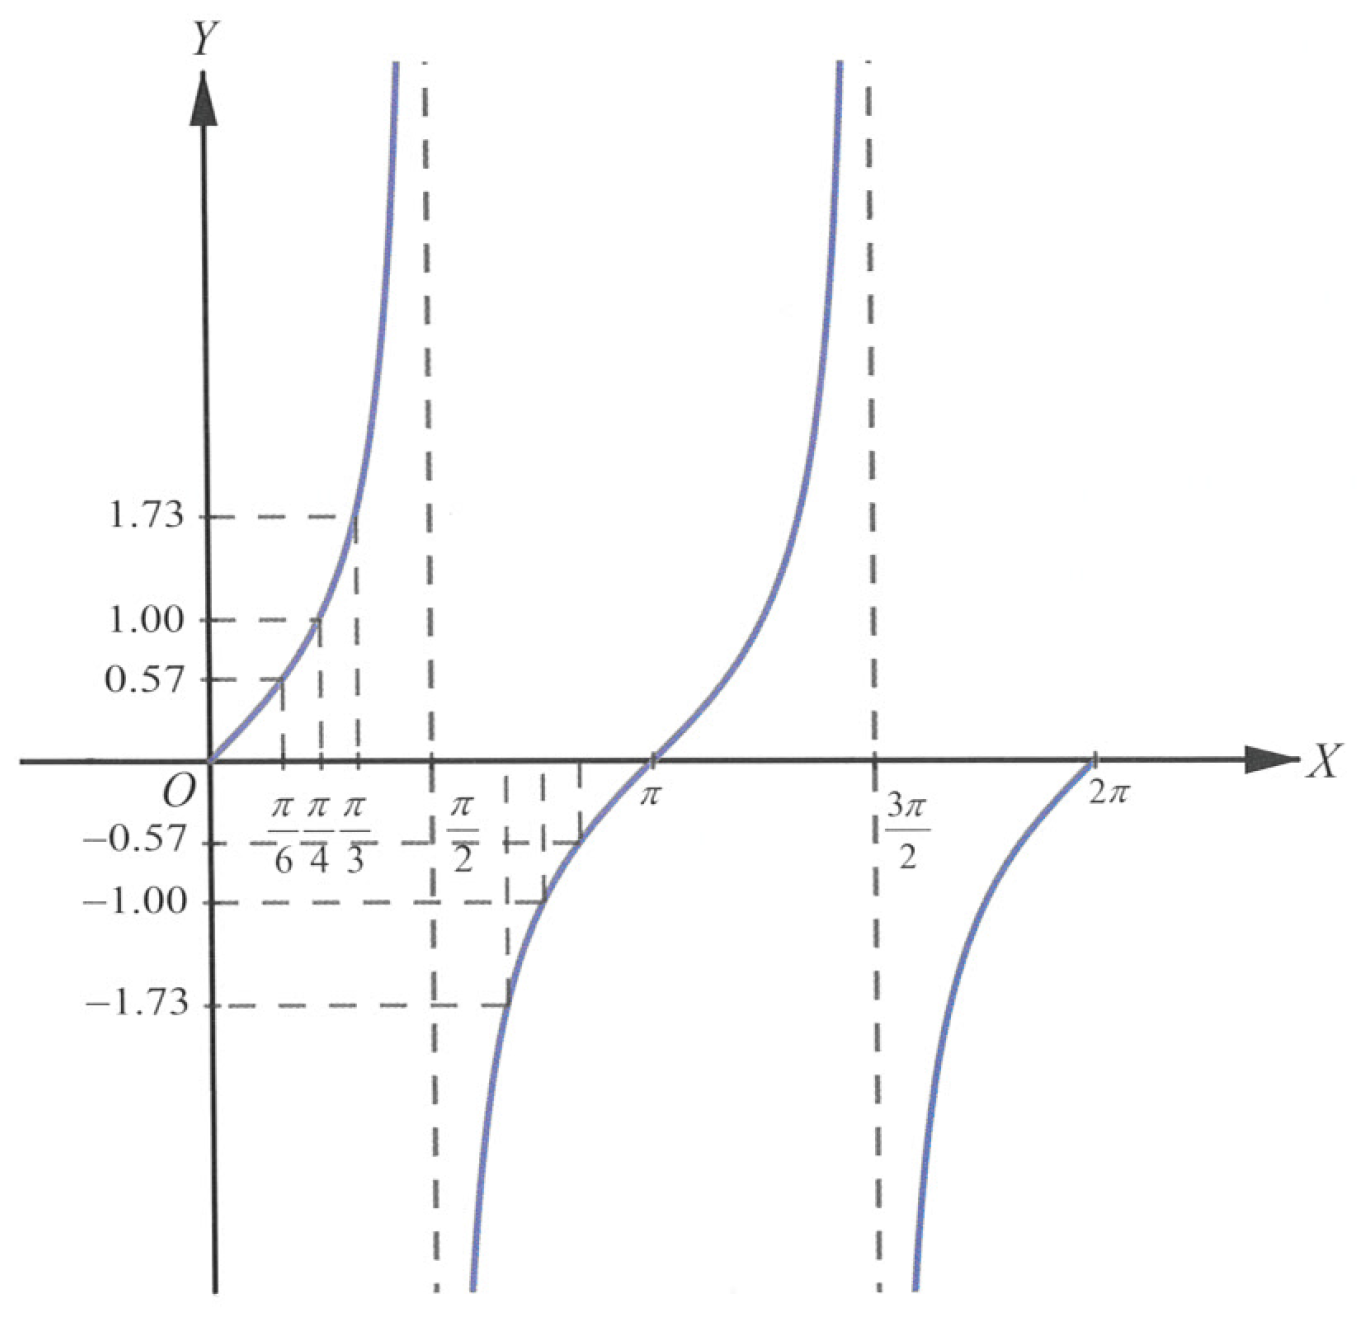
\includegraphics[scale=0.5]{39} 
	\caption{} 
	\label{Figure39} 
\end{figure}
จากรูป จะเห็นว่า เมื่อ $x$ มีค่าเพิ่มขึ้นจาก $0$ และเข้าใกล้ $\dfrac{\pi}{2}$ ค่าของ $\tan x$ จะเป็นจำนวนจริงบวก และเพิ่มขึ้นเรื่อย ๆ โดยเส้นกราฟจะโค้งเข้าหาเส้นตรง $x=\dfrac{\pi}{2}$ แต่ $\tan x$ ไม่นิยามที่ $x=\dfrac{\pi}{2}$ เมื่อ $x$ มีค่าลดลงจาก $\pi$ และเข้าใกล้ $\dfrac{\pi}{2}$ ค่าของ $\tan x$ จะเป็นจำนวนจริงลบและลดลงเรื่อย ๆ โดยเส้นกราฟจะโค้งเข้าหาเส้นตรง $x=\dfrac{\pi}{2}$ ในทำนองเดียวกัน เมื่อ $x$ มีค่าเพิ่มขึ้นจาก $\pi$ และเข้าใกล้ $\dfrac{3 \pi}{2}$ ค่าของ $\tan x$ จะเป็นจำนวนจริงบวก และเพิ่มขึ้นเรื่อย ๆ โดยเส้นกราฟจะโค้งเข้าหาเส้นตรง $x=\dfrac{3 \pi}{2}$ แต่ $\tan x$ ไม่นิยามที่ $x=\dfrac{3 \pi}{2}$

\vspace{0.5em}
เมื่อ $x$ มีค่าลดลงจาก $2 \pi$ และเข้าใกล้ $\dfrac{3 \pi}{2}$ ค่าของ $\tan x$ จะเป็นจำนวนจริงลบและลดลงเรื่อย ๆ โดยเส้นกราฟจะโค้งเข้าหาเส้นตรง $x=\dfrac{3 \pi}{2}$

\vspace{0.5em}
ดังนั้น ในการเขียนกราฟดังกล่าว ถ้าลากเส้นประ $x=\dfrac{\pi}{2}$ และ $x=\dfrac{3 \pi}{2}$ ก่อน จะช่วยให้เขียนกราฟ ได้ง่ายขึ้น แต่เส้นประดังกล่าวนั้นมิได้เป็นส่วนหนึ่งของกราฟ

\vspace{0.5em}
เนื่องจาก $\tan (n \pi+\theta)=\tan \theta$ เมื่อ $n$ เป็นจำนวนเต็มใด ๆ กราฟของฟังก์ชันแทนเจนต์จึงมีลักษณะ ซ้ำกันเป็นช่วง ๆ ดังนั้น ฟังก์ชันแทนเจนต์จึงเป็นฟังก์ชันที่เป็นคาบ

\vspace{0.5em}
จะได้ กราฟของ $y=\tan x$ เป็นดังนี้
\begin{figure}[H] 
	\centering 
	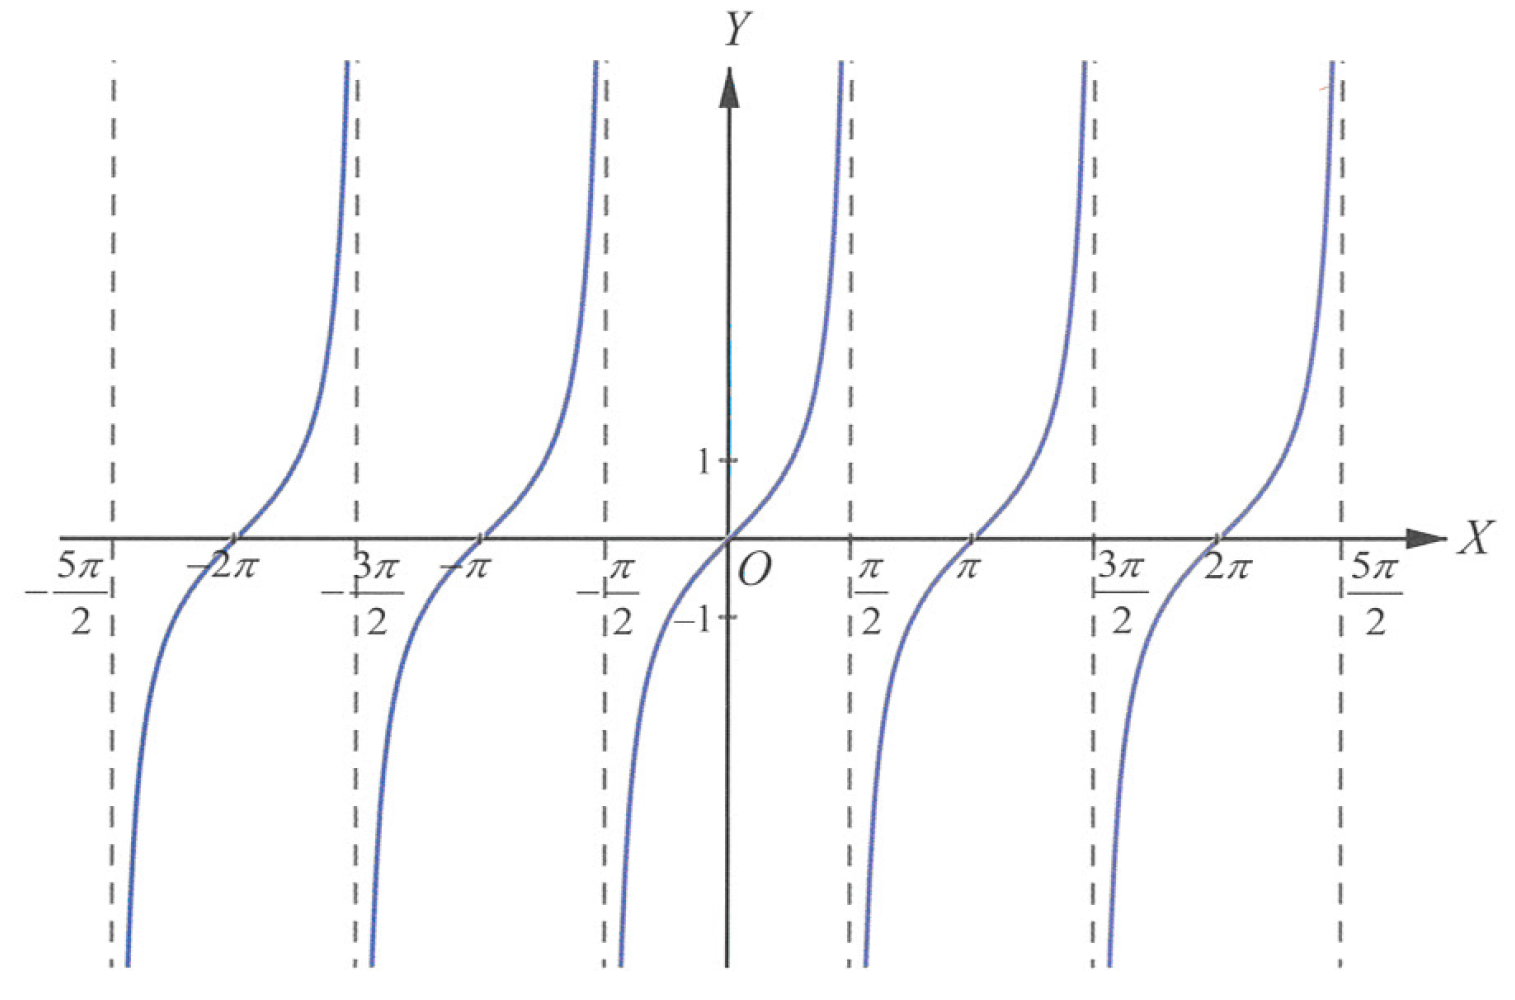
\includegraphics[scale=0.55]{40} 
	\caption{} 
	\label{Figure40} 
\end{figure}

จากรูป จะเห็นว่า ฟังก์ชันแทนเจนต์เป็นฟังก์ชันที่เป็นคาบและมีคาบเท่ากับ $\pi$

\vspace{0.5em}
เนื่องจากค่าของฟังก์ชันโคเซแคนต์ ฟังก์ชันเซแคนต์ และฟังก์ชันโคแทนเจนต์ที่ $x$ เป็นส่วนกลับของ ค่าของฟังก์ชันไซน์ ฟังก์ชันโคไซน์ และฟังก์ชันแทนเจนต์ที่ $x$ ตามลำดับ จึงสามารถเขียนกราฟของ ฟังก์ชันโคเซแคนต์ ฟังก์ชันเซแคนต์ และฟังก์ชันโคแทนเจนต์ ได้ดังนี้

\vspace{1em}
\noindent กราฟของ $y=\operatorname{cosec} x$
\begin{figure}[H] 
	\centering 
	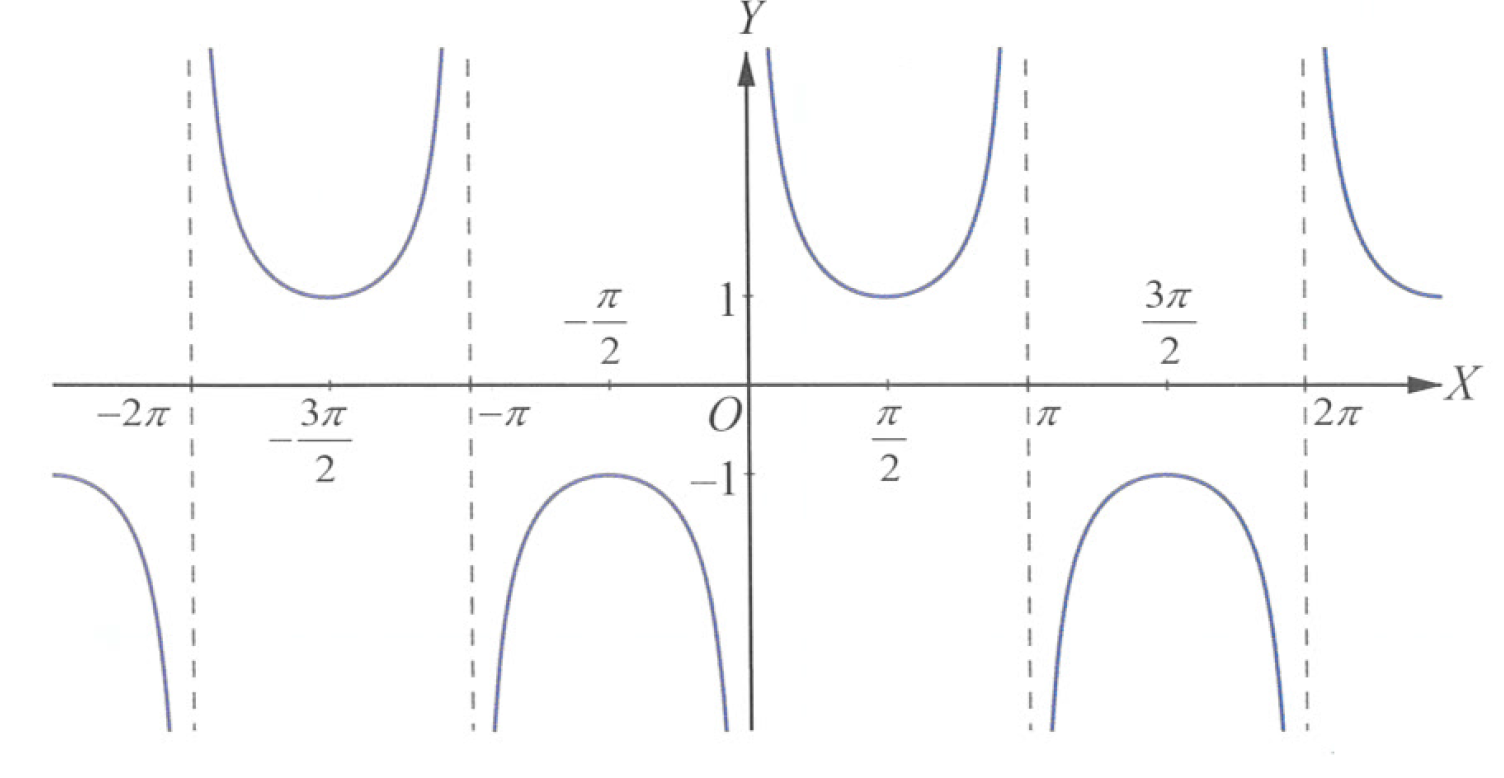
\includegraphics[scale=0.55]{41} 
	\caption{} 
	\label{Figure41} 
\end{figure}

จากรูป จะเห็นว่า ฟังก์ชันโคเซแคนต์เป็นฟังก์ชันที่เป็นคาบและมีคาบเท่ากับ $2 \pi$

\newpage
\noindent กราฟของ $y=\sec x$
\begin{figure}[H] 
	\centering 
	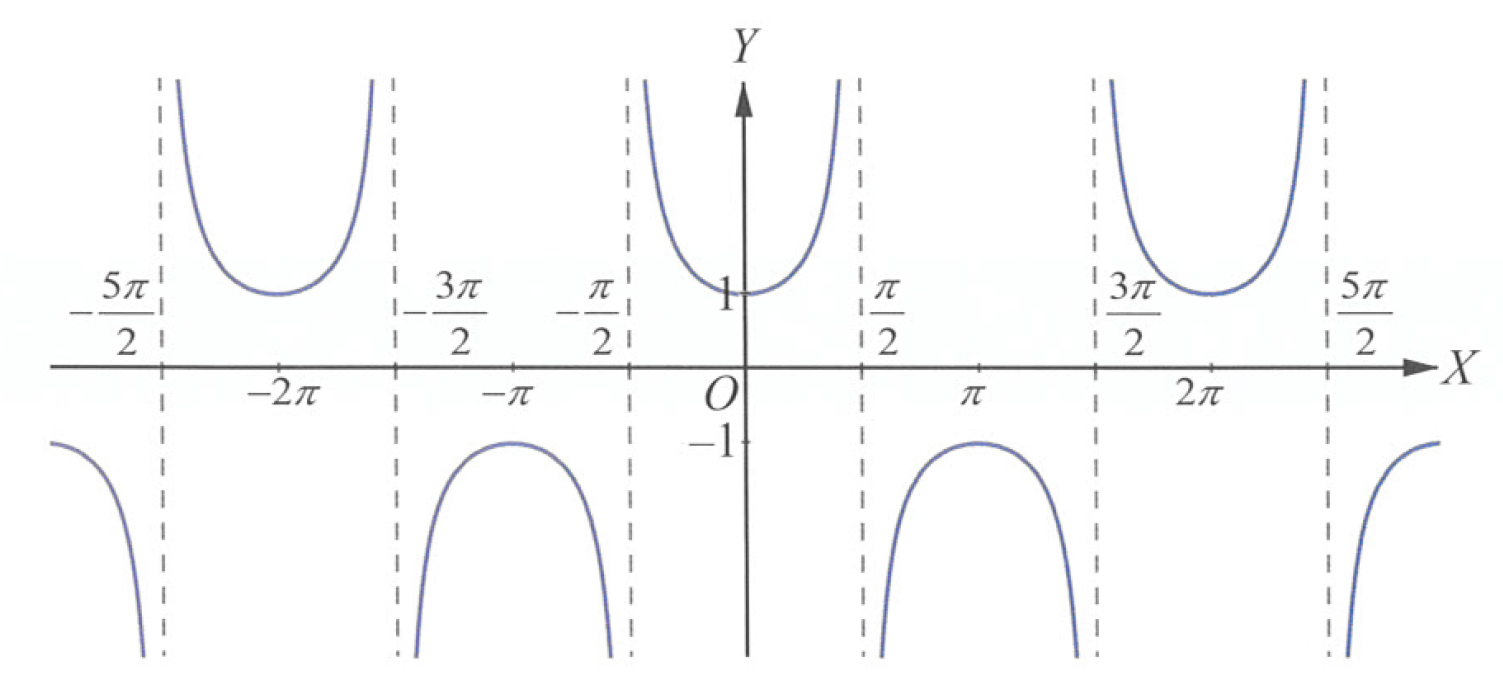
\includegraphics[scale=0.55]{42} 
	\caption{} 
	\label{Figure42} 
\end{figure}
จากรูป จะเห็นว่า ฟังก์ชันเซแคนต์เป็นฟังก์ชันที่เป็นคาบและมีคาบเท่ากับ $2 \pi$

กราฟของ $y=\cot x$
\begin{figure}[H] 
	\centering 
	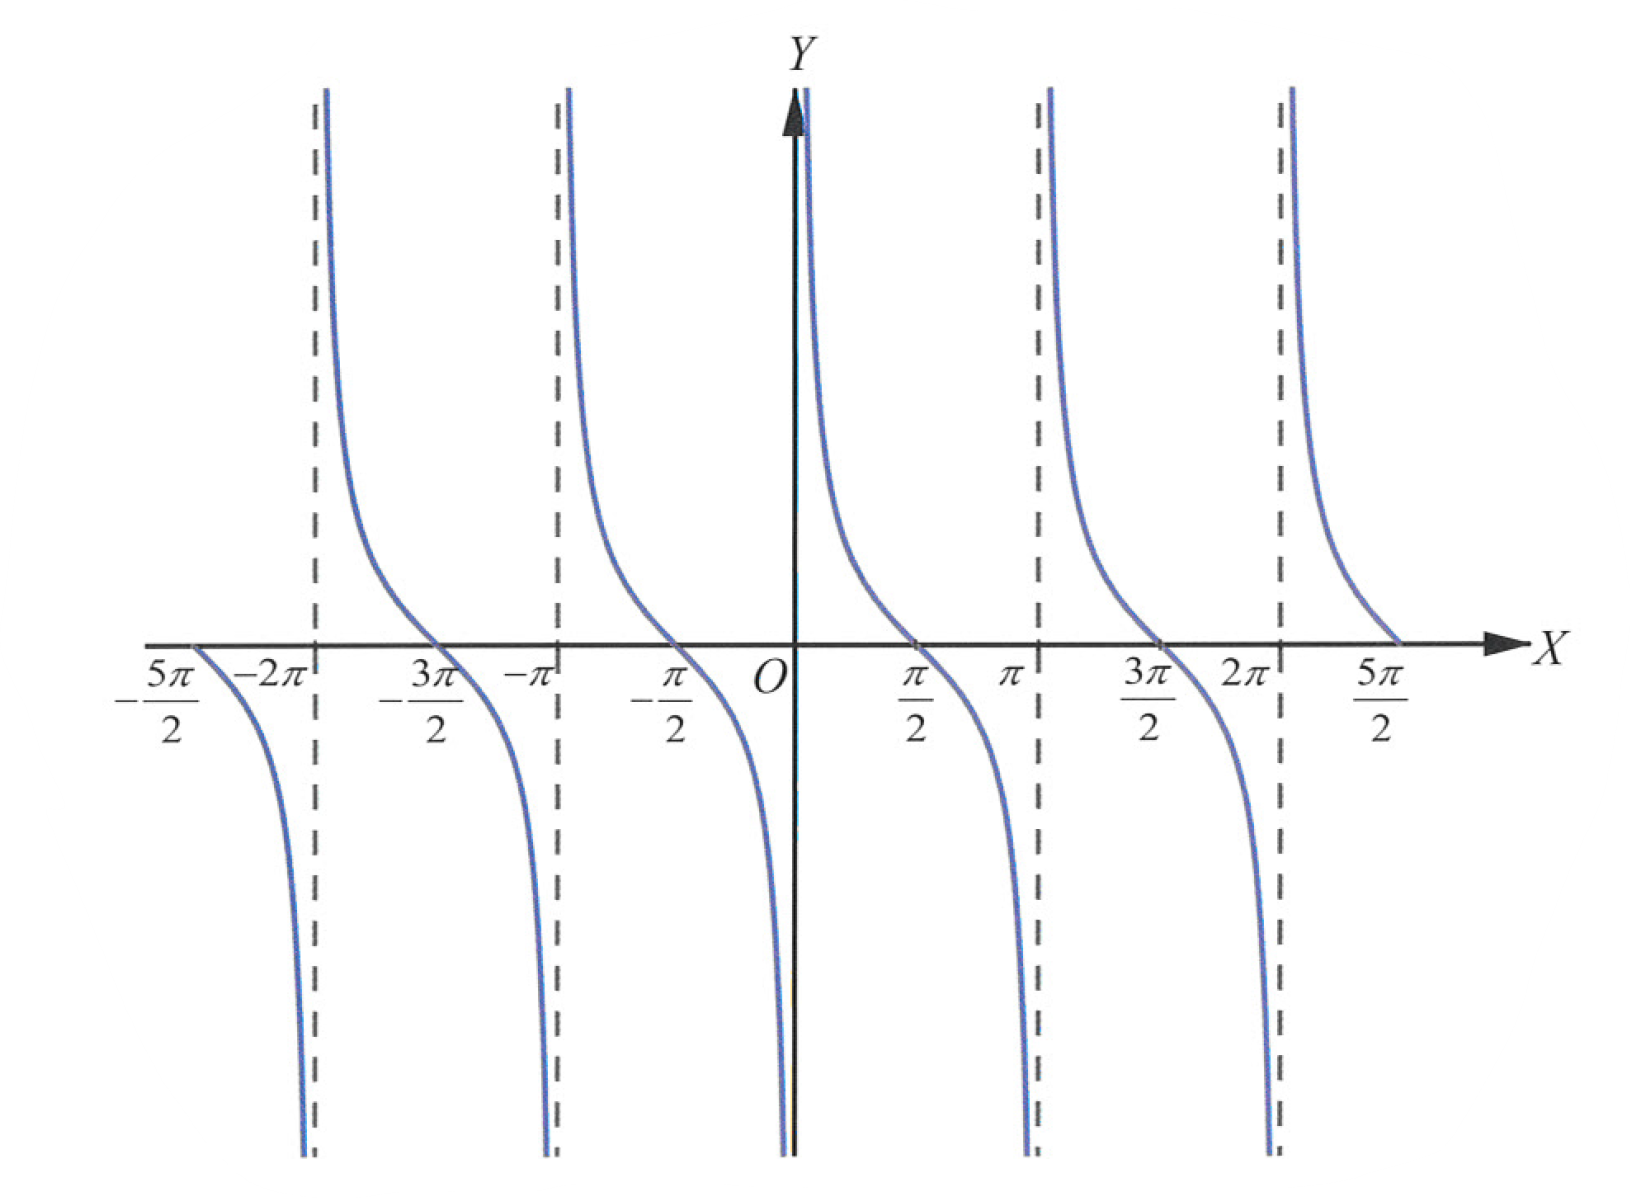
\includegraphics[scale=0.55]{43} 
	\caption{} 
	\label{Figure43} 
\end{figure}

จากรูป จะเห็นว่า ฟังก์ชันโคแทนเจนต์เป็นฟังก์ชันที่เป็นคาบและมีคาบเท่ากับ $\pi$

\newpage
\section{ฟังก์ชันตรีโกณมิติของผลบวกและผลต่างของ จำนวนจริงหรือมุม}
ในหัวข้อนี้จะศึกษาฟังก์ชันตรีโกณมิติของผลบวกและผลต่างของจำนวนจริงหรือมุม โดยสิ่งแรก ที่จะพิจารณา คือ ค่าของฟังก์ชันโคไซน์ของผลต่างระหว่างจำนวนจริงสองจำนวน หรือมุมสองมุม นั่นคือ พิจารณาค่าของ $\cos (\alpha-\beta)$ เมื่อ $\alpha$ และ $\beta$ เป็นจำนวนจริงหรือมุมใด ๆ
\\
\begin{figure}[H] 
	\centering 
	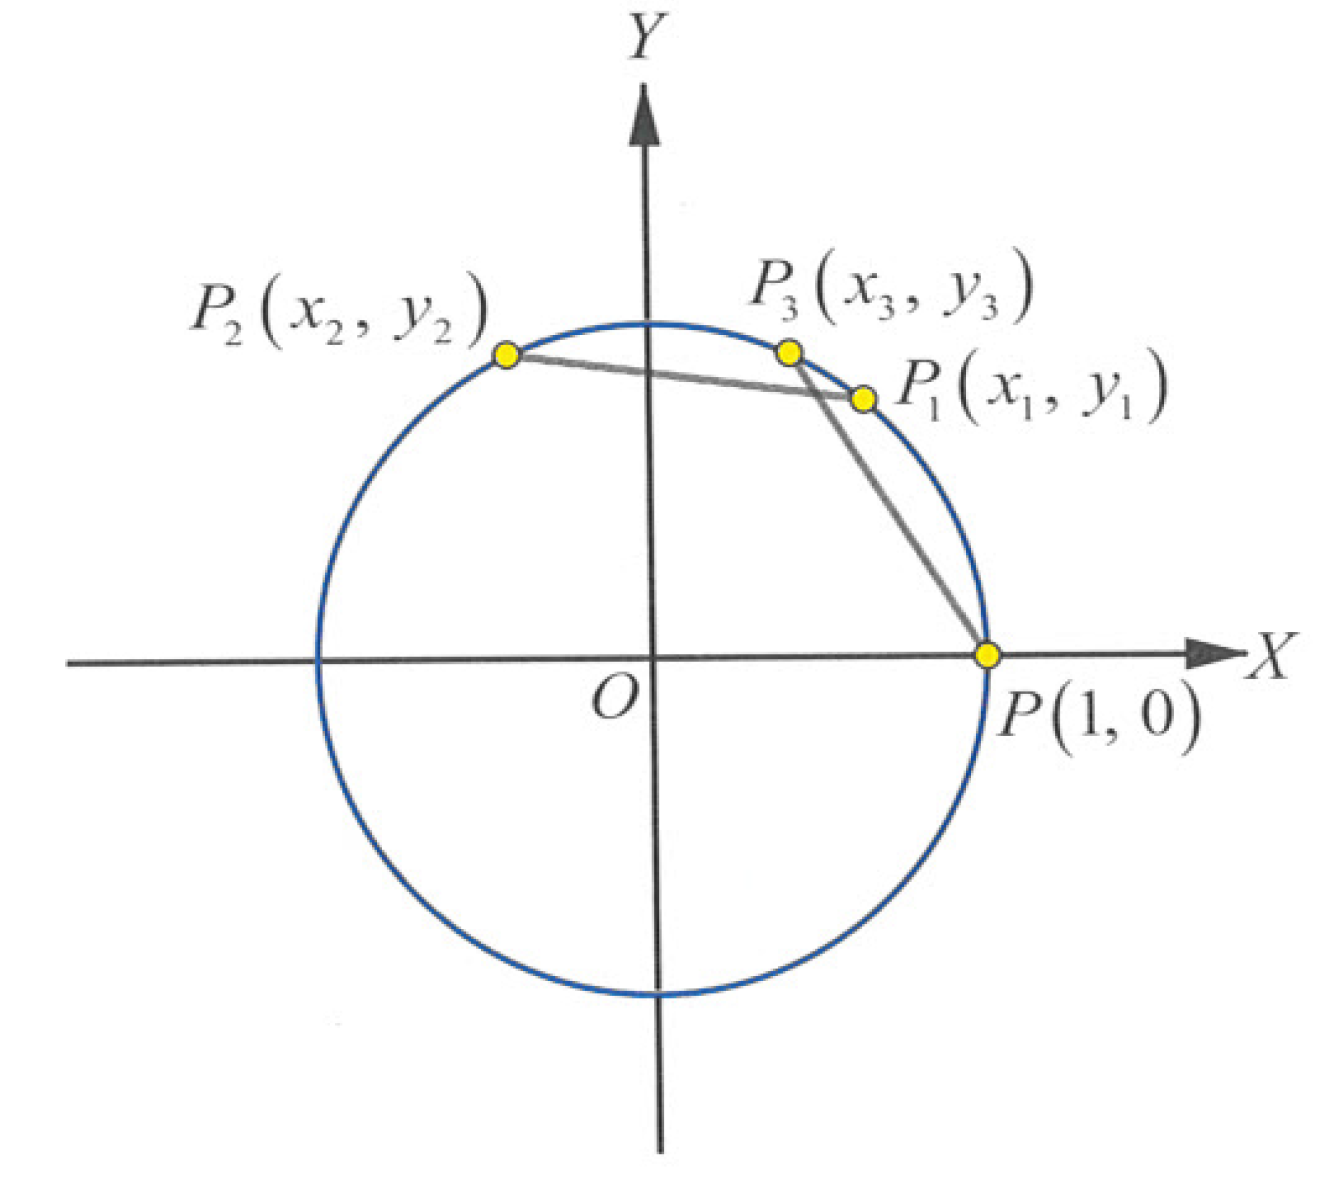
\includegraphics[scale=0.55]{44} 
	\caption{} 
	\label{Figure44} 
\end{figure}

\noindent กำหนดให้ $P$, $P_{1}$ และ $P_{2}$ เป็นจุดบนวงกลมหนึ่งหน่วย
\\
ให้ส่วนโค้ง $P P_{1}$ ยาว $\beta$ หน่วย และส่วนโค้ง $P P_{2}$ ยาว $\alpha$ หน่วย
\\
ดังนั้น ส่วนโค้ง $P_{1} P_{2}$ ยาว $\alpha-\beta$ หน่วย
\\
ให้ $P_{3}$ เป็นจุดบนวงกลมหนึ่งหน่วยที่ทำให้ส่วนโค้ง $P P_{3}$ ยาวเท่ากับส่วนโค้ง $P_{1} P_{2}$
\\
ดังนั้น ส่วนโค้ง $P P_{3}$ ยาว $\alpha-\beta$ หน่วย
\\
ให้พิกัดของจุด $P_{1}$, $P_{2}$ และ $P_{3}$ เป็น $(x_{1}, y_{1})$, $(x_{2}, y_{2})$ และ $(x_{3}, y_{3})$ ตามลำดับ เนื่องจากส่วนโค้ง $P P_{3}$ ยาวเท่ากับส่วนโค้ง $P_{1} P_{2}$
\\
ดังนั้น คอร์ด $P P_{3}$ ยาวเท่ากับคอร์ด $P_{1} P_{2}$

\vspace{0.5em}
\noindent นั่นคือ
$$
\begin{aligned}
	\left(P P_{3}\right)^{2} & =\left(P_{1} P_{2}\right)^{2} \\
	\left(x_{3}-1\right)^{2}+\left(y_{3}-0\right)^{2} & =\left(x_{2}-x_{1}\right)^{2}+\left(y_{2}-y_{1}\right)^{2} \\
	x_{3}^{2}-2 x_{3}+1+y_{3}^{2} & =x_{2}^{2}-2 x_{2} x_{1}+x_{1}^{2}+y_{2}^{2}-2 y_{2} y_{1}+y_{1}^{2} \\
	-2 x_{3}+2 & =-2 x_{2} x_{1}-2 y_{2} y_{1}+2 \quad \text { เพราะจุด } (x_{1}, y_{1}), (x_{2}, y_{2}) \\
	& \text { และ } (x_{3}, y_{3}) \text { อยู่บนวงกลม } \\
	& \text { หนึ่งหน่วย }
\end{aligned}
$$

\begin{equation*}
	x_{3}=x_{2} x_{1}+y_{2} y_{1} \tag{1}
\end{equation*}

\noindent เนื่องจากจุด $(x_{1}, y_{1})$, $(x_{2}, y_{2})$ และ $(x_{3}, y_{3})$ เป็นจุดปลายส่วนโค้งที่ยาว $\beta$, $\alpha$ และ $\alpha-\beta$ หน่วย ตามลำดับ
\\
จะได้
$$
\begin{array}{ll}
	x_{1}=\cos \beta, & y_{1}=\sin \beta \\
	x_{2}=\cos \alpha, & y_{2}=\sin \alpha \\
	x_{3}=\cos (\alpha-\beta) &
\end{array}
$$

\noindent จากสมการ (1) จะได้ $\cos (\alpha-\beta)=\cos \alpha \cos \beta+\sin \alpha \sin \beta$

\vspace{0.5em}
\noindent ที่กล่าวมาข้างต้นเป็นการหา $\cos (\alpha-\beta)$ หรือโคไซน์ของผลต่างระหว่างจำนวนจริงสองจำนวนหรือ มุมสองมุม ที่กล่าวถึงก่อนเพราะหาได้ง่ายและสามารถนำไปใช้ในการหา $\cos (\alpha+\beta)$, $\sin (\alpha+\beta)$ และ $\sin (\alpha-\beta)$ ซึ่งหาได้ดังนี้
$$
\begin{aligned}
	\cos (\alpha+\beta) & = \cos (\alpha-(-\beta)) \\
	& = \cos \alpha \cos (-\beta)+\sin \alpha \sin (-\beta) \\
	& = \cos \alpha \cos \beta+\sin \alpha(-\sin \beta) \\
	& = \cos \alpha \cos \beta-\sin \alpha \sin \beta
\end{aligned}
$$

\noindent ดังนั้น $\cos (\alpha+\beta)=\cos \alpha \cos \beta-\sin \alpha \sin \beta$
\\
ในการหา $\sin (\alpha+\beta)$ อาจทำได้โดยพิสูจน์ว่า $\cos \left( \dfrac{\pi}{2}-\alpha \right)=\sin \alpha$ และ $\sin \left( \dfrac{\pi}{2}-\beta \right)=\cos \beta$ ก่อนดังนี้ เนื่องจาก $\cos \left( \dfrac{\pi}{2}-\alpha \right)=\cos \dfrac{\pi}{2} \cos \alpha+\sin \dfrac{\pi}{2} \sin \alpha$
$$
=\sin \alpha
$$
ดังนั้น
$$
\cos \left( \dfrac{\pi}{2}-\alpha \right)=\sin \alpha
$$
ให้ $\gamma=\dfrac{\pi}{2}-\beta$
\\
จะได้
$$
\cos \left( \dfrac{\pi}{2}-\gamma \right)=\cos \left( \dfrac{\pi}{2}-\left( \dfrac{\pi}{2}-\beta \right) \right)
$$
เนื่องจาก
$$
\cos \left( \dfrac{\pi}{2}-\gamma \right)=\sin \gamma
$$
ดังนั้น
$$
\sin \gamma=\cos \beta
$$
นั่นคือ
$$
\sin \left( \dfrac{\pi}{2}-\beta \right)=\cos \beta
$$
เนื่องจาก
$$
\begin{aligned}
	\sin (\alpha+\beta) & = \cos \left( \dfrac{\pi}{2}-(\alpha+\beta) \right) \\
	& = \cos \left( \left( \dfrac{\pi}{2}-\alpha \right)-\beta \right) \\
	& = \cos \left( \dfrac{\pi}{2}-\alpha \right) \cos \beta+\sin \left( \dfrac{\pi}{2}-\alpha \right) \sin \beta \\
	& = \sin \alpha \cos \beta+\cos \alpha \sin \beta
\end{aligned}
$$
ดังนั้น $\sin (\alpha+\beta)=\sin \alpha \cos \beta+\cos \alpha \sin \beta$

\vspace{0.5em}
\noindent เนื่องจาก
$$
\begin{aligned}
	\sin (\alpha-\beta) & = \sin (\alpha+(-\beta)) \\
	& = \sin \alpha \cos (-\beta)+\cos \alpha \sin (-\beta) \\
	& = \sin \alpha \cos \beta+\cos \alpha(-\sin \beta) \\
	& = \sin \alpha \cos \beta-\cos \alpha \sin \beta
\end{aligned}
$$
ดังนั้น $\sin (\alpha-\beta)=\sin \alpha \cos \beta-\cos \alpha \sin \beta$

\vspace{0.5em}
\noindent เมื่อทราบค่าของ $\sin (\alpha+\beta)$ และ $\cos (\alpha+\beta)$ แล้วจะสามารถหาค่าของ $\tan (\alpha+\beta)$ ได้ดังนี้
$$
\begin{aligned}
	\tan (\alpha+\beta) & = \dfrac{\sin (\alpha+\beta)}{\cos (\alpha+\beta)} \quad \text{เมื่อ } \cos (\alpha+\beta) \neq 0 \\
	& = \dfrac{\sin \alpha \cos \beta+\cos \alpha \sin \beta}{\cos \alpha \cos \beta-\sin \alpha \sin \beta} \\
	& = \dfrac{\dfrac{\sin \alpha \cos \beta}{\cos \alpha \cos \beta}+\dfrac{\cos \alpha \sin \beta}{\cos \alpha \cos \beta}}{\dfrac{\cos \alpha \cos \beta}{\cos \alpha \cos \beta}-\dfrac{\sin \alpha \sin \beta}{\cos \alpha \cos \beta}} \quad \text{เมื่อ } \cos \alpha \cos \beta \neq 0
\end{aligned}
$$
ดังนั้น $\tan (\alpha+\beta)=\dfrac{\tan \alpha+\tan \beta}{1-\tan \alpha \tan \beta}$ เมื่อ $\tan \alpha \tan \beta \neq 1$
\\
ในทำนองเดียวกัน จะได้ว่า $\tan (\alpha-\beta)=\dfrac{\tan \alpha-\tan \beta}{1+\tan \alpha \tan \beta}$ เมื่อ $\tan \alpha \tan \beta \neq -1$

\vspace{0.5em}
\noindent สรุปค่าของฟังก์ชันตรีโกณมิติของผลบวกและผลต่างของจำนวนจริงหรือมุมได้ดังนี้
$$
\begin{aligned}
	\cos (\alpha-\beta) & = \cos \alpha \cos \beta+\sin \alpha \sin \beta \\
	\cos (\alpha+\beta) & = \cos \alpha \cos \beta-\sin \alpha \sin \beta \\
	\sin (\alpha-\beta) & = \sin \alpha \cos \beta-\cos \alpha \sin \beta \\
	\sin (\alpha+\beta) & = \sin \alpha \cos \beta+\cos \alpha \sin \beta \\
	\tan (\alpha-\beta) & = \dfrac{\tan \alpha-\tan \beta}{1+\tan \alpha \tan \beta} \quad \text{เมื่อ } \tan \alpha \tan \beta \neq -1 \\
	\tan (\alpha+\beta) & = \dfrac{\tan \alpha+\tan \beta}{1-\tan \alpha \tan \beta} \quad \text{เมื่อ } \tan \alpha \tan \beta \neq 1
\end{aligned}
$$

\newpage
การหาค่าของฟังก์ชันตรีโกณมิติของจำนวนจริงหรือมุมโดยใช้ฟังก์ชันตรีโกณมิติของผลบวกและผลต่างของจำนวนจริงหรือมุมทำได้ดังนี้
\begin{examplebox}
	จงหาค่าของ $\cos \left( \dfrac{3 \pi}{4}-\dfrac{\pi}{3} \right)$
\end{examplebox}
\solution
\vspace{6cm}

\begin{examplebox}
	จงหาค่าของ $\sin \left( \dfrac{\pi}{9} \right) \cos \left( \dfrac{\pi}{18} \right)+\cos \left( \dfrac{\pi}{9} \right) \sin \left( \dfrac{\pi}{18} \right)$
\end{examplebox}
\solution
\newpage
\begin{examplebox}
	จงหาค่าของ $\sin 15^{\circ}$ และ $\cos 75^{\circ}$
\end{examplebox}
\solution
\vspace{6cm}

\begin{examplebox}
	จงหาค่าของ $\tan \left( \dfrac{7 \pi}{12} \right)$
\end{examplebox}
\solution
\newpage

\begin{examplebox}
	จงแสดงว่า $\tan \left( \theta+\dfrac{\pi}{2} \right)=-\cot \theta$
\end{examplebox}
\solution จาก $\tan \theta=\dfrac{\sin \theta}{\cos \theta}$

$$
\text{จะได้ } \begin{aligned}
	\tan \left( \theta+\dfrac{\pi}{2} \right) & = \dfrac{\sin \left( \theta+\dfrac{\pi}{2} \right)}{\cos \left( \theta+\dfrac{\pi}{2} \right)} \\
	& = \dfrac{\sin \theta \cos \left( \dfrac{\pi}{2} \right)+\cos \theta \sin \left( \dfrac{\pi}{2} \right)}{\cos \theta \cos \left( \dfrac{\pi}{2} \right)-\sin \theta \sin \left( \dfrac{\pi}{2} \right)} \\
	& = \dfrac{(\sin \theta)(0)+(\cos \theta)(1)}{(\cos \theta)(0)-(\sin \theta)(1)} \\
	& = \dfrac{\cos \theta}{-\sin \theta} \\
	& = -\cot \theta
\end{aligned}
$$

\remark จากตัวอย่างข้างต้น ไม่สามารถใช้ $\tan (\alpha+\beta)=\dfrac{\tan \alpha+\tan \beta}{1-\tan \alpha \tan \beta}$ ได้ เนื่องจาก $\tan \beta$ ไม่นิยามที่ $\beta=\dfrac{\pi}{2}$
\newpage

\begin{examplebox}
ให้ $\sin \alpha = \dfrac{4}{5}$ เมื่อ $\dfrac{\pi}{2} < \alpha < \pi$ และ $\sin \beta = -\dfrac{2}{\sqrt{5}}$ เมื่อ $\pi < \beta < \dfrac{3 \pi}{2}$ จงหาค่าของ
\begin{enumerate}
	\item $\cos \alpha$
	\item $\cos \beta$
	\item $\cos (\alpha+\beta)$
	\item $\sin (\alpha+\beta)$
\end{enumerate}
\end{examplebox}
\solution

\newpage
จากค่าของ $\sin (\alpha+\beta)$, $\sin (\alpha-\beta)$, $\cos (\alpha+\beta)$ และ $\cos (\alpha-\beta)$ เมื่อนำมาบวกหรือลบกันจะได้ ความสัมพันธ์ที่สำคัญดังต่อไปนี้

$$
\begin{aligned}
	2 \sin \alpha \cos \beta & = \sin (\alpha+\beta)+\sin (\alpha-\beta) \\
	2 \cos \alpha \sin \beta & = \sin (\alpha+\beta)-\sin (\alpha-\beta) \\
	2 \cos \alpha \cos \beta & = \cos (\alpha+\beta)+\cos (\alpha-\beta) \\
	2 \sin \alpha \sin \beta & = \cos (\alpha-\beta)-\cos (\alpha+\beta)
\end{aligned}
$$

\begin{examplebox}
จงหาค่าของ $\cos 75^{\circ} \sin 525^{\circ}$
\end{examplebox}
\solution
\newpage

นอกจากนี้ยังสามารถหาความสัมพันธ์อื่น ๆ ได้ดังนี้

$$
\begin{aligned}
	\sin \alpha+\sin \beta & = 2 \sin \left( \dfrac{\alpha+\beta}{2} \right) \cos \left( \dfrac{\alpha-\beta}{2} \right) \\
	\sin \alpha-\sin \beta & = 2 \cos \left( \dfrac{\alpha+\beta}{2} \right) \sin \left( \dfrac{\alpha-\beta}{2} \right) \\
	\cos \alpha+\cos \beta & = 2 \cos \left( \dfrac{\alpha+\beta}{2} \right) \cos \left( \dfrac{\alpha-\beta}{2} \right) \\
	\cos \alpha-\cos \beta & = -2 \sin \left( \dfrac{\alpha+\beta}{2} \right) \sin \left( \dfrac{\alpha-\beta}{2} \right)
\end{aligned}
$$

\begin{examplebox}
จงหาค่าของ $\sin 75^{\circ}+\sin 15^{\circ}$
\end{examplebox}
\solution
\newpage

\begin{examplebox}
	จงหาค่าของ $\cos \left( \dfrac{17 \pi}{12} \right)+\cos \left( \dfrac{11 \pi}{12} \right)$
\end{examplebox}
\solution
\newpage

เมื่อทราบค่าของ $\sin \alpha$, $\cos \alpha$ หรือ $\tan \alpha$ จะสามารถหาค่าของฟังก์ชันตรีโกณมิติของจำนวนซึ่ง เป็นสองเท่าของ $\alpha$ ได้ โดยอาศัยค่าของ $\sin (\alpha+\beta)$, $\cos (\alpha+\beta)$ และ $\tan (\alpha+\beta)$ ตามลำดับ เช่น หาค่าของ $\sin 2 \alpha$ ได้ดังนี้
\\
เนื่องจาก
$$
\begin{aligned}
	\sin 2 \alpha & = \sin (\alpha+\alpha) \\
	& = \sin \alpha \cos \alpha+\cos \alpha \sin \alpha
\end{aligned}
$$
ดังนั้น
$$
\sin 2 \alpha = 2 \sin \alpha \cos \alpha
$$

\noindent นอกจากนี้ยังสามารถหาค่าของ $\cos 2 \alpha$ จาก $\cos (\alpha+\beta)$ ได้ดังนี้
$$
\begin{aligned}
	\cos 2 \alpha & = \cos (\alpha+\alpha) \\
	& = \cos \alpha \cos \alpha-\sin \alpha \sin \alpha
\end{aligned}
$$
ดังนั้น
\begin{equation*}
	\cos 2 \alpha = \cos ^{2} \alpha-\sin ^{2} \alpha \tag{1}
\end{equation*}

\noindent แทน $\cos ^{2} \alpha$ ด้วย $1-\sin ^{2} \alpha$ ใน $(1)$ จะได้
$$
\begin{aligned}
	\cos 2 \alpha & = \left(1-\sin ^{2} \alpha\right)-\sin ^{2} \alpha \\
	\cos 2 \alpha & = 1-2 \sin ^{2} \alpha
\end{aligned}
$$
และแทน $\sin ^{2} \alpha$ ด้วย $1-\cos ^{2} \alpha$ ใน $(1)$ จะได้
$$
\cos 2 \alpha = \cos ^{2} \alpha-\left(1-\cos ^{2} \alpha\right)
$$
ดังนั้น
$$
\cos 2 \alpha = 2 \cos ^{2} \alpha-1
$$

\noindent และสามารถหาค่าของ $\tan 2 \alpha$ โดยใช้ $\tan (\alpha+\beta)$ ดังนี้
$$
\begin{aligned}
	\tan 2 \alpha & = \tan (\alpha+\alpha) \\
	& = \dfrac{\tan \alpha+\tan \alpha}{1-\tan \alpha \tan \alpha}
\end{aligned}
$$
ดังนั้น
$$
\tan 2 \alpha = \dfrac{2 \tan \alpha}{1-\tan ^{2} \alpha} \quad \text{เมื่อ } \tan ^{2} \alpha \neq 1
$$

\vspace{0.5em}
\noindent สรุปความสัมพันธ์ที่กล่าวมาได้ดังนี้
$$
\begin{aligned}
	\sin 2 \alpha & = 2 \sin \alpha \cos \alpha \\
	\cos 2 \alpha & = \cos ^{2} \alpha-\sin ^{2} \alpha \\
	\cos 2 \alpha & = 1-2 \sin ^{2} \alpha \\
	\cos 2 \alpha & = 2 \cos ^{2} \alpha-1 \\
	\tan 2 \alpha & = \dfrac{2 \tan \alpha}{1-\tan ^{2} \alpha} \quad \text{เมื่อ } \tan ^{2} \alpha \neq 1
\end{aligned}
$$

\newpage

\begin{examplebox}
กำหนดให้ $\cos \theta = \dfrac{3}{5}$ และ $\sin \theta < 0$ จงหาค่าของ
\begin{enumerate}
	\item $\sin 2 \theta$
	\item $\cos 2 \theta$
	\item $\tan 2 \theta$
\end{enumerate}
\end{examplebox}
\solution
\newpage

\begin{examplebox}
	จงแสดงว่า $\cot x \sin 2 x=1+\cos 2 x$ เมื่อ $\sin x \neq 0$
\end{examplebox}
\solution $\cot x \sin 2 x = \dfrac{\cos x}{\sin x}(\sin 2 x)$ เมื่อ $\sin x \neq 0$

$$
\begin{aligned}
	& = \dfrac{\cos x}{\sin x}(2 \sin x \cos x) \\
	& = 2 \cos ^{2} x \\
	& = 1+\cos 2 x
\end{aligned}
$$

\begin{examplebox}
	จงเขียน $\sin 3 \alpha$ ในรูปของ $\sin \alpha$
\end{examplebox}
\solution จาก $\sin (\alpha+\beta)=\sin \alpha \cos \beta+\cos \alpha \sin \beta$
\\
จะได้ $\sin 3 \alpha = \sin (2 \alpha+\alpha)$

$$
\begin{aligned}
	& = \sin 2 \alpha \cos \alpha+\cos 2 \alpha \sin \alpha \\
	& = (2 \sin \alpha \cos \alpha) \cos \alpha+\left(\cos ^{2} \alpha-\sin ^{2} \alpha\right) \sin \alpha \\
	& = 2 \sin \alpha \cos ^{2} \alpha+\cos ^{2} \alpha \sin \alpha-\sin ^{3} \alpha \\
	& = 2 \sin \alpha\left(1-\sin ^{2} \alpha\right)+\left(1-\sin ^{2} \alpha\right) \sin \alpha-\sin ^{3} \alpha \\
	& = 2 \sin \alpha-2 \sin ^{3} \alpha+\sin \alpha-\sin ^{3} \alpha-\sin ^{3} \alpha \\
	& = 3 \sin \alpha-4 \sin ^{3} \alpha
\end{aligned}
$$

\newpage
\section{ตัวผกผันของฟังก์ชันตรีโกณมิติ}
การหาตัวผกผันของฟังก์ชันทำได้โดยการสลับที่ระหว่างสมาชิกตัวหน้าและสมาชิกตัวหลังของแต่ละ คู่อันดับที่เป็นสมาชิกของฟังก์ชัน โดยฟังก์ชัน $1-1$ เท่านั้นที่มีตัวผกผันเป็นฟังก์ชัน

เนื่องจากฟังก์ชันตรีโกณมิติไม่เป็นฟังก์ชัน $1-1$ ดังนั้น ตัวผกผันของฟังก์ชันตรีโกณมิติจึงไม่เป็นฟังก์ชัน เช่น ฟังก์ชันไซน์มีคู่อันดับ $(0,0),(\pi, 0)$ และ $(2 \pi, 0)$ เป็นสมาชิก ดังนั้น คู่อันดับ $(0,0),(0, \pi)$ และ $(0,2 \pi)$ จึงเป็นสมาชิกของตัวผกผันของฟังก์ชันไซน์ ซึ่งจะพบว่าตัวผกผันของฟังก์ชันไซน์ไม่เป็น ฟังก์ชัน แต่ถ้ากำหนดโดเมนของฟังก์ชันตรีโกณมิติให้เหมาะสม จะพบว่าตัวผกผันของฟังก์ชันตรีโกณมิติ จะเป็นฟังก์ชัน

\subsection*{ตัวผกผันของฟังก์ชันไซน์}
พิจารณากราฟของ $y=\sin x$ เมื่อ $-\infty < x < \infty$ และ $-1 \leq y \leq 1$ และกราฟของความสัมพันธ์ $\{(x, y) \mid x=\sin y\}$ ซึ่งเป็นตัวผกผันของฟังก์ชันไซน์ต่อไปนี้

\begin{figure}[H] 
	\centering 
	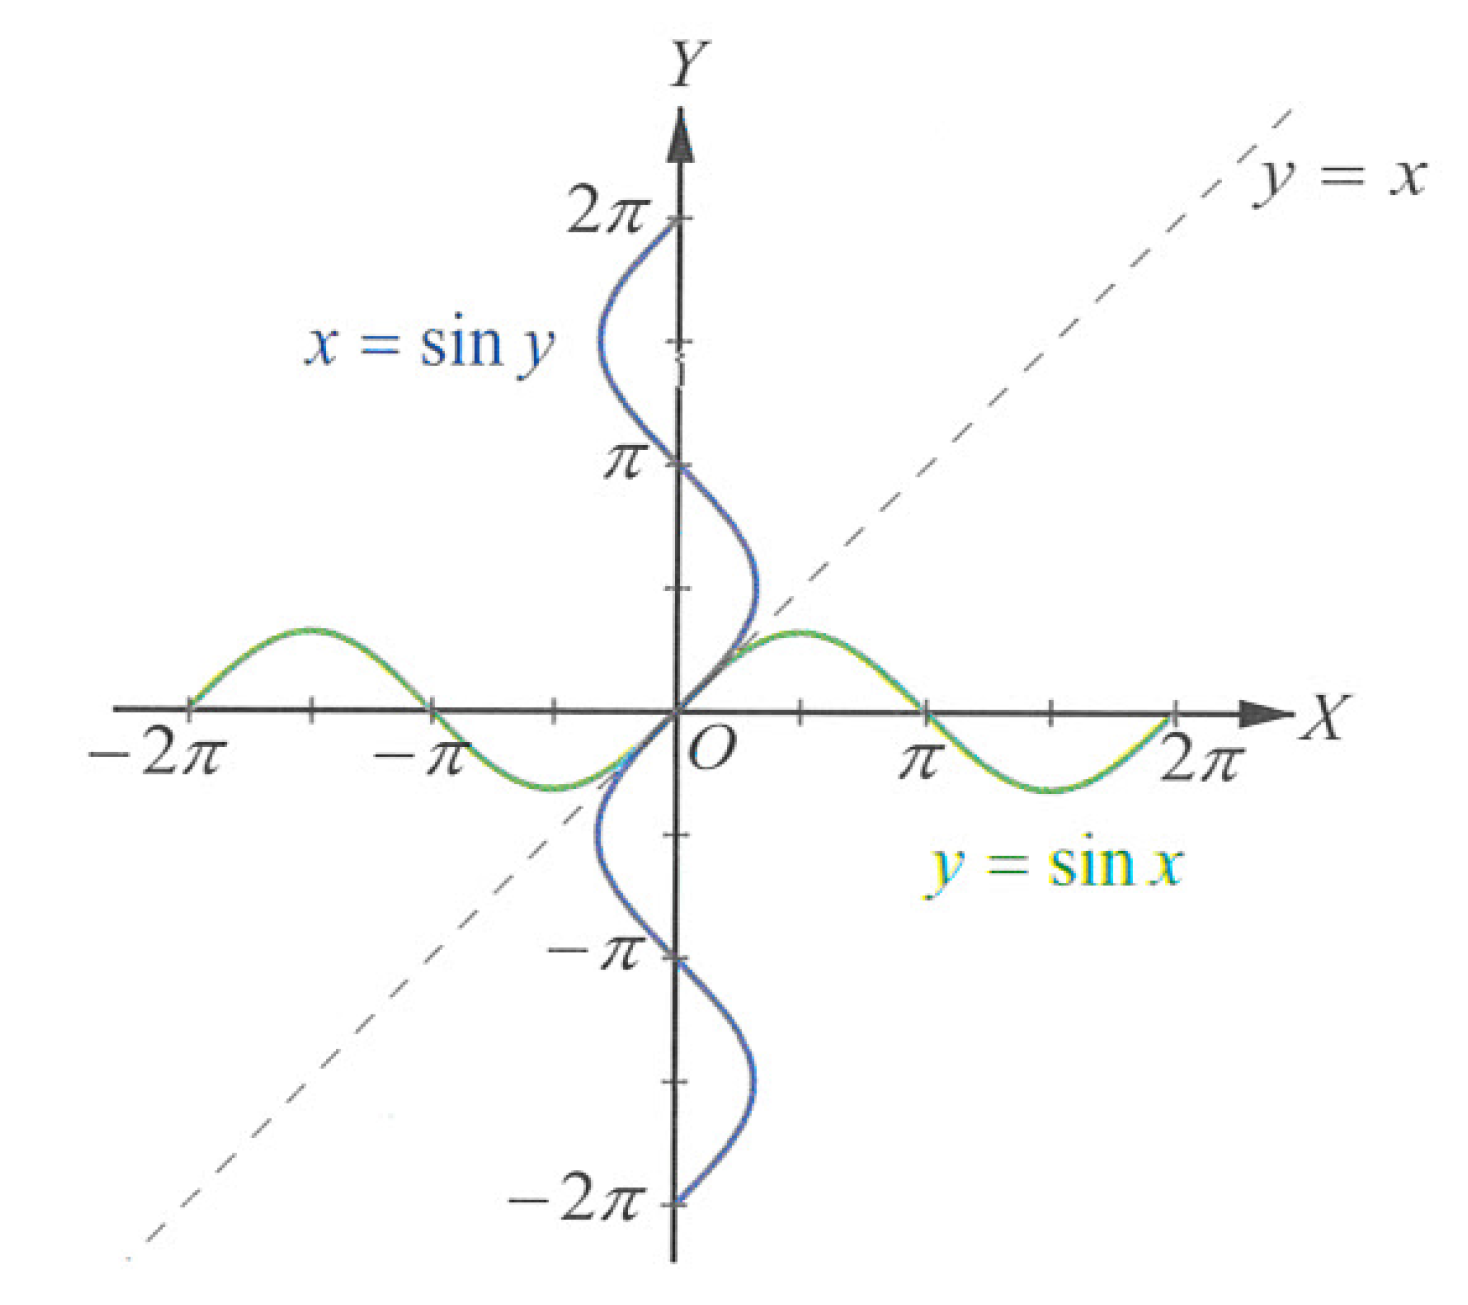
\includegraphics[scale=0.55]{45} 
	\caption{} 
	\label{Figure45} 
\end{figure}

\noindent จะเห็นว่า $\{(x, y) \mid x=\sin y\}$ ไม่เป็นฟังก์ชัน แต่ถ้ากำหนดโดเมนของฟังก์ชันไซน์เป็น $\left[ -\dfrac{\pi}{2}, \dfrac{\pi}{2} \right]$ จะได้ว่า
$$
\left\{ (x, y) \;\middle|\; y=\sin x, -\dfrac{\pi}{2} \leq x \leq \dfrac{\pi}{2} \right\}
$$
เป็นฟังก์ชัน $1-1$ ซึ่งมีฟังก์ชันผกผันเป็น
$$
\left\{ (x, y) \;\middle|\; x=\sin y, -\dfrac{\pi}{2} \leq y \leq \dfrac{\pi}{2} \right\}
$$
และจะเรียกฟังก์ชันผกผันนี้ว่า $\arcsin$

\begin{definitionbox}
	ฟังก์ชัน $\arcsin$ คือ เซตของคู่อันดับ $(x, y)$ โดยที่ $x=\sin y$ และ $-\dfrac{\pi}{2} \leq y \leq \dfrac{\pi}{2}$
\end{definitionbox}

\noindent เมื่อ $(x, y) \in \text{arcsine}$ จะได้ $y=\arcsin x$ ซึ่งมีความหมายเช่นเดียวกับ $x=\sin y$ เมื่อ $-\dfrac{\pi}{2} \leq y \leq \dfrac{\pi}{2}$

\vspace{0.5em}
\noindent พิจารณากราฟของฟังก์ชัน $\left\{ (x, y) \;\middle|\; y=\sin x, -\dfrac{\pi}{2} \leq x \leq \dfrac{\pi}{2} \right\}$ และกราฟของฟังก์ชัน
$$
\left\{ (x, y) \;\middle|\; y=\arcsin x, -1 \leq x \leq 1 \right\}
$$

\begin{figure}[H] 
	\centering 
	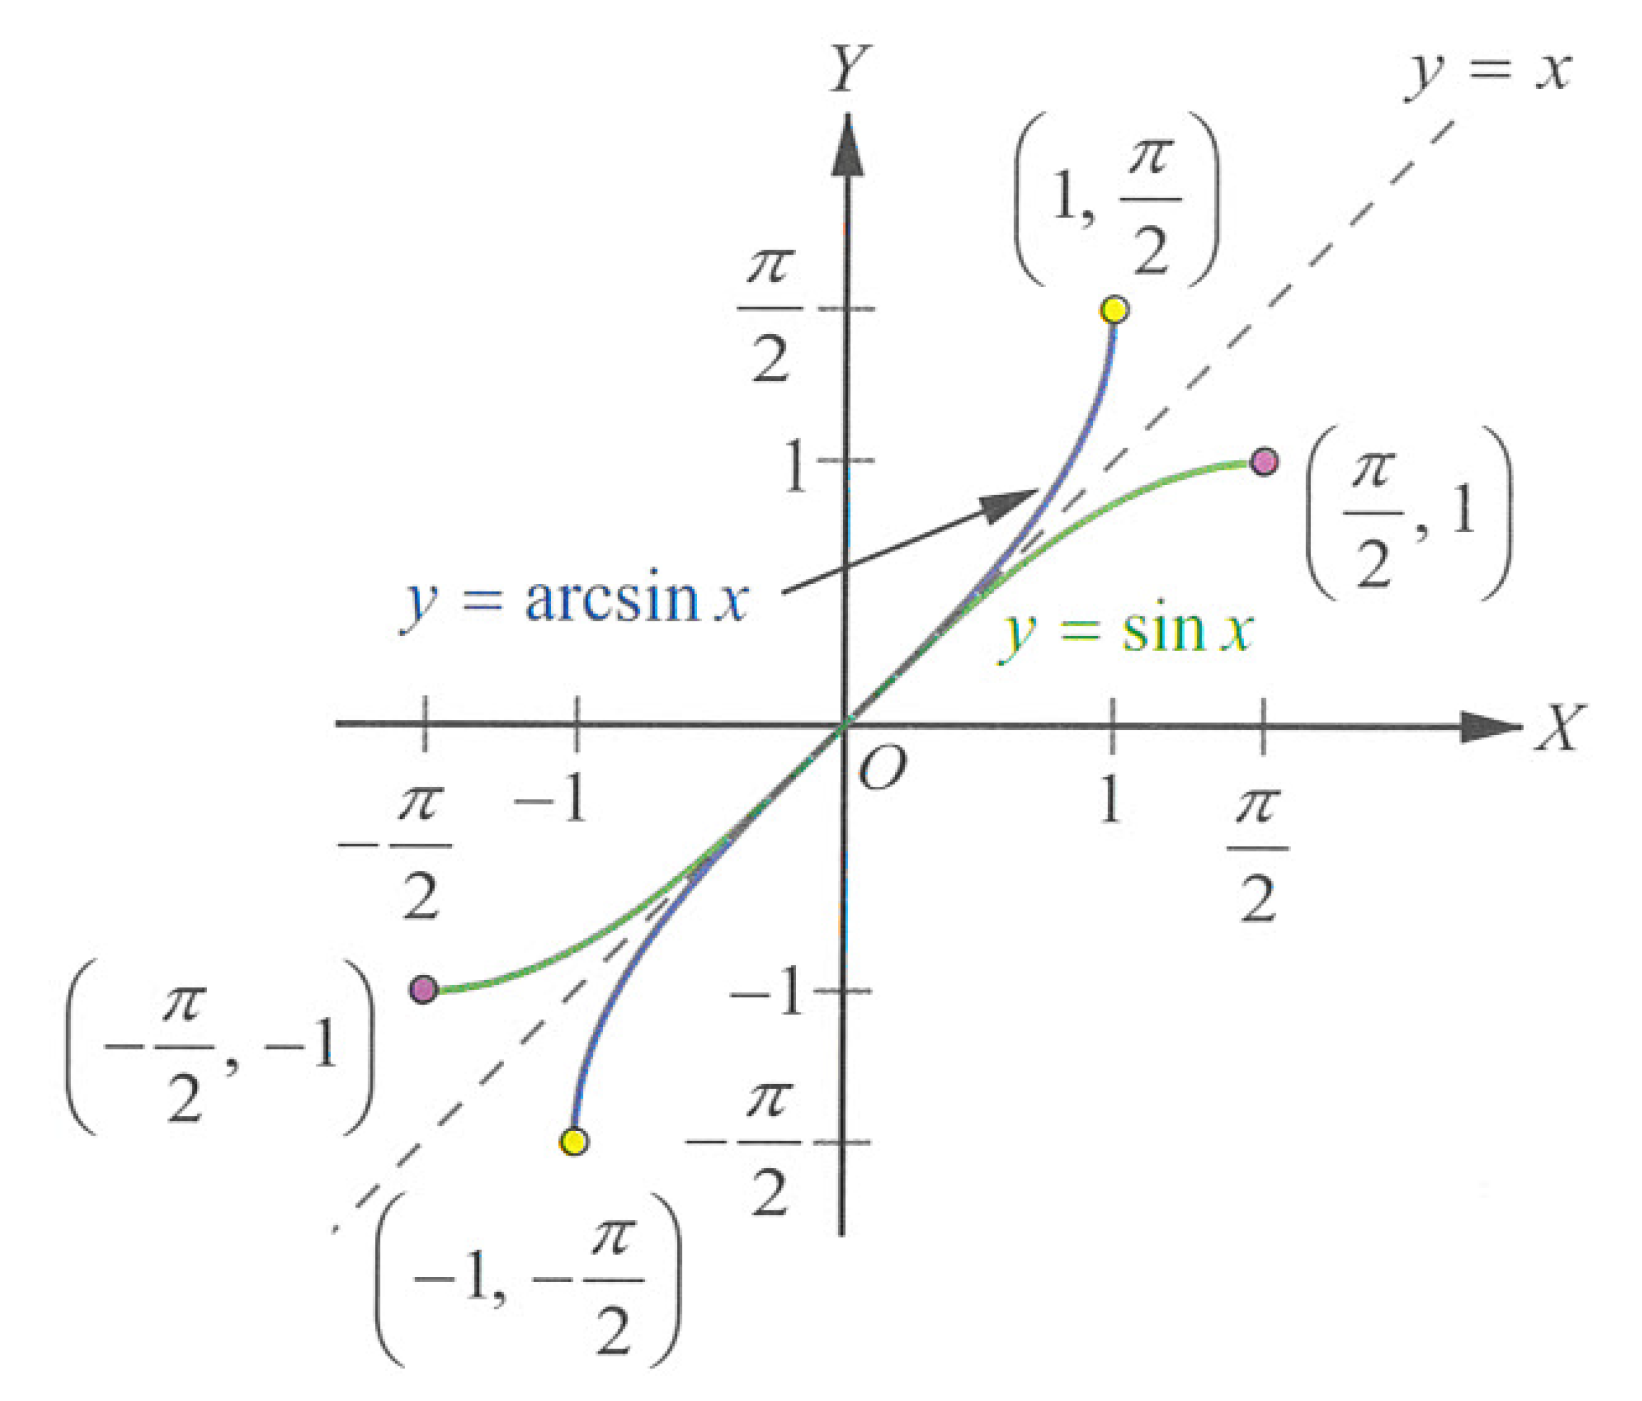
\includegraphics[scale=0.55]{46} 
	\caption{} 
	\label{Figure46} 
\end{figure}
จะเห็นว่า โดเมนของฟังก์ชัน $\arcsin$ คือ $[-1,1]$ และเรนจ์ของฟังก์ชัน $\arcsin$ คือ $\left[ -\dfrac{\pi}{2}, \dfrac{\pi}{2} \right]$


การหาค่าของฟังก์ชันผกผันของฟังก์ชันตรีโกณมิติสามารถทำได้โดยอาศัยฟังก์ชันตรีโกณมิตินั้น ๆ เช่น การหาค่าของ $\arcsin x$ โดยที่ $-1 \leq x \leq 1$ ก็คือการหา $\theta$ ซึ่งอยู่ในเรนจ์ของฟังก์ชัน $\arcsin$ ที่ทำให้ $\sin \theta=x$ นั่นเอง
\begin{examplebox}
	จงหาค่าของ $\arcsin 1$
\end{examplebox}
\solution
\vspace{5cm}
\begin{examplebox}
	จงหาค่าของ $\arcsin \left( \dfrac{\sqrt{3}}{2} \right)$
\end{examplebox}
\solution
\vspace{5cm}
\begin{examplebox}
	จงหาค่าของ $\arcsin \left( -\dfrac{1}{2} \right)$
\end{examplebox}
\solution
\newpage

\subsection*{ตัวผกผันของฟังก์ชันโคไซน์}
พิจารณากราฟของฟังก์ชัน $y=\cos x$

\begin{figure}[H] 
	\centering 
	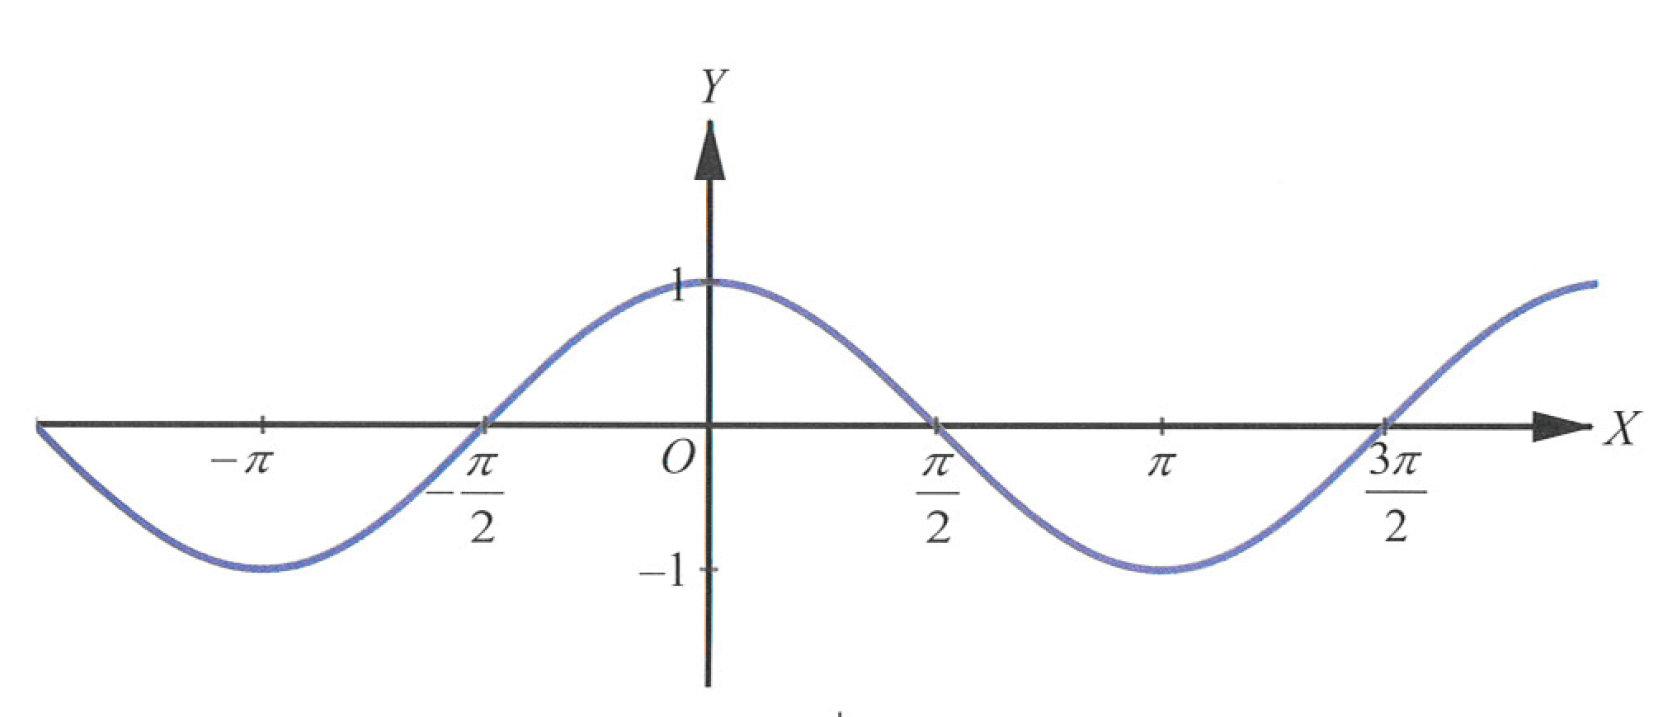
\includegraphics[scale=0.55]{47} 
	\caption{} 
	\label{Figure47} 
\end{figure}

\noindent เมื่อกำหนดโดเมนของ $y=\cos x$ เป็น $[0, \pi]$ จะได้ว่า
$$
\left\{ (x, y) \;\middle|\; y=\cos x, 0 \leq x \leq \pi \right\}
$$
เป็นฟังก์ชัน $1-1$ ซึ่งมีฟังก์ชันผกผันเป็น
$$
\left\{ (x, y) \;\middle|\; x=\cos y, 0 \leq y \leq \pi \right\}
$$
เรียกฟังก์ชันผกผันนี้ว่า arccosine

\begin{definitionbox}
	ฟังก์ชัน arccosine คือ เซตของคู่อันดับ $(x, y)$ โดยที่ $x=\cos y$ และ $0 \leq y \leq \pi$
\end{definitionbox}

\noindent เมื่อ $(x, y) \in \text{arccosine}$ จะได้ $y=\arccos x$ ซึ่งมีความหมายเช่นเดียวกับ $x=\cos y$ เมื่อ $0 \leq y \leq \pi$

\vspace{0.5em}
พิจารณากราฟของฟังก์ชัน $\left\{ (x, y) \;\middle|\; y=\cos x, 0 \leq x \leq \pi \right\}$ และกราฟของฟังก์ชัน
$$
\left\{ (x, y) \;\middle|\; y=\arccos x, -1 \leq x \leq 1 \right\}
$$
\begin{figure}[H] 
	\centering 
	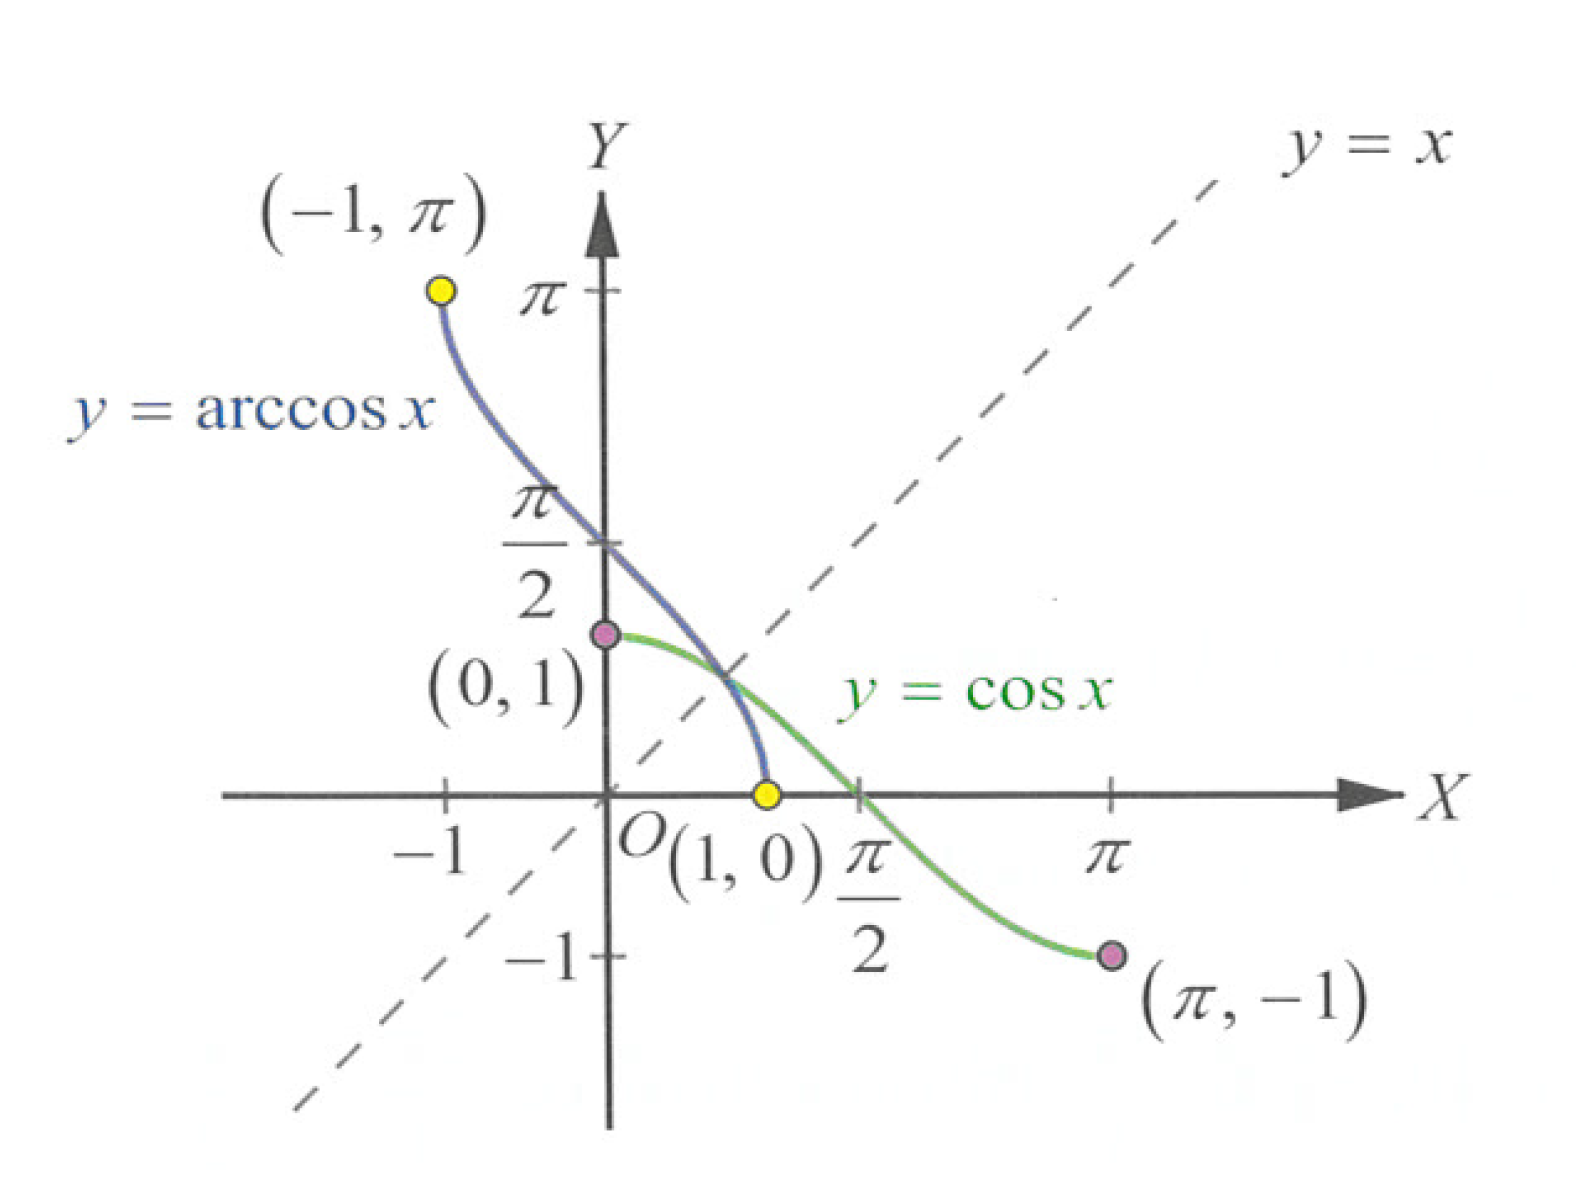
\includegraphics[scale=0.55]{48} 
	\caption{} 
	\label{Figure48} 
\end{figure}
จะเห็นว่า โดเมนของฟังก์ชัน arccosine คือ $[-1,1]$ และเรนจ์ของฟังก์ชัน arccosine คือ $[0, \pi]$

\begin{examplebox}
จงหาค่าของ $\arccos 0$
\end{examplebox}
\solution
\newpage

\begin{examplebox}
จงหาค่าของ $\arccos \left(-\frac{1}{2}\right)$
\end{examplebox}
\newpage

\subsection*{ตัวผกผันของฟังก์ชันแทนเจนต์}
พิจารณากราฟของฟังก์ชัน $y=\tan x$

\begin{figure}[H] 
	\centering 
	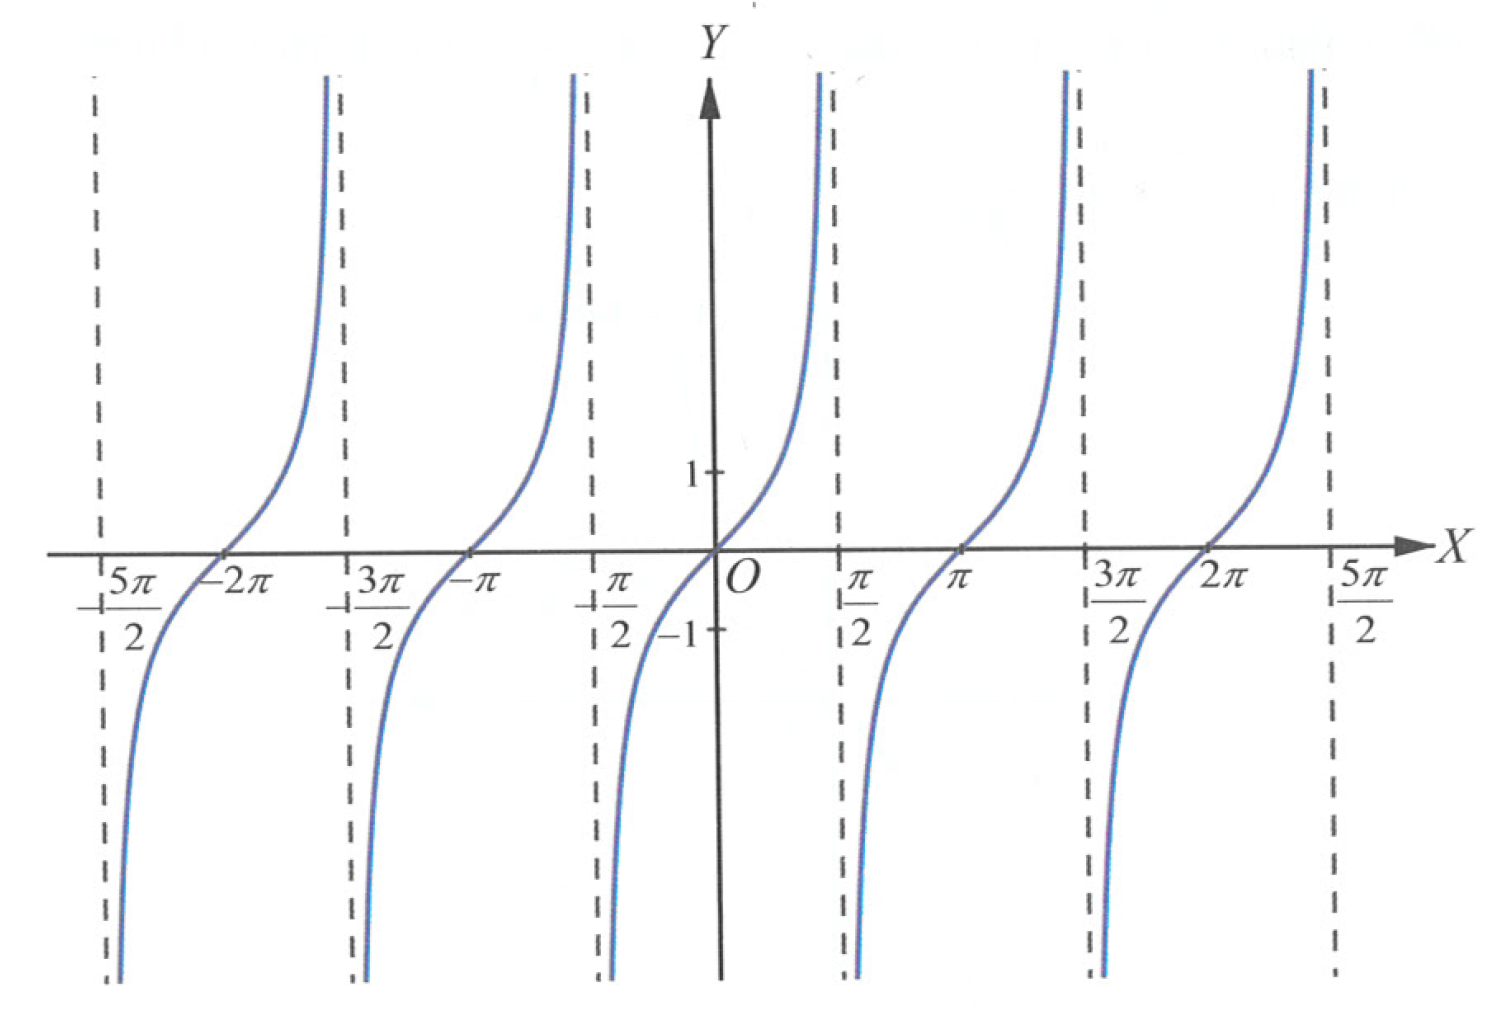
\includegraphics[scale=0.55]{49} 
	\caption{} 
	\label{Figure49} 
\end{figure}

\noindent เมื่อกำหนดโดเมนของ $y=\tan x$ เป็น $\left( -\dfrac{\pi}{2}, \dfrac{\pi}{2} \right)$ จะได้ว่า ฟังก์ชัน
$$
\left\{ (x, y) \;\middle|\; y=\tan x, -\dfrac{\pi}{2} < x < \dfrac{\pi}{2} \right\}
$$
เป็นฟังก์ชัน $1-1$ ซึ่งมีฟังก์ชันผกผันเป็น
$$
\left\{ (x, y) \;\middle|\; x=\tan y, -\dfrac{\pi}{2} < y < \dfrac{\pi}{2} \right\}
$$
เรียกฟังก์ชันผกผันนี้ว่า arctangent

\begin{definitionbox}
	ฟังก์ชัน arctangent คือ เซตของคู่อันดับ $(x, y)$ โดยที่ $x=\tan y$ และ $-\dfrac{\pi}{2} < y < \dfrac{\pi}{2}$
\end{definitionbox}

\noindent เมื่อ $(x, y) \in \text{arctangent}$ จะได้ $y=\arctan x$ ซึ่งมีความหมายเช่นเดียวกับ $x=\tan y$ เมื่อ $-\dfrac{\pi}{2} < y < \dfrac{\pi}{2}$ 
\newline
พิจารณากราฟของฟังก์ชัน $\left\{ (x, y) \;\middle|\; y=\tan x, -\dfrac{\pi}{2} < x < \dfrac{\pi}{2} \right\}$ และกราฟของฟังก์ชัน
$$
\left\{ (x, y) \;\middle|\; y=\arctan x, -\infty < x < \infty \right\}
$$

\begin{figure}[H] 
	\centering 
	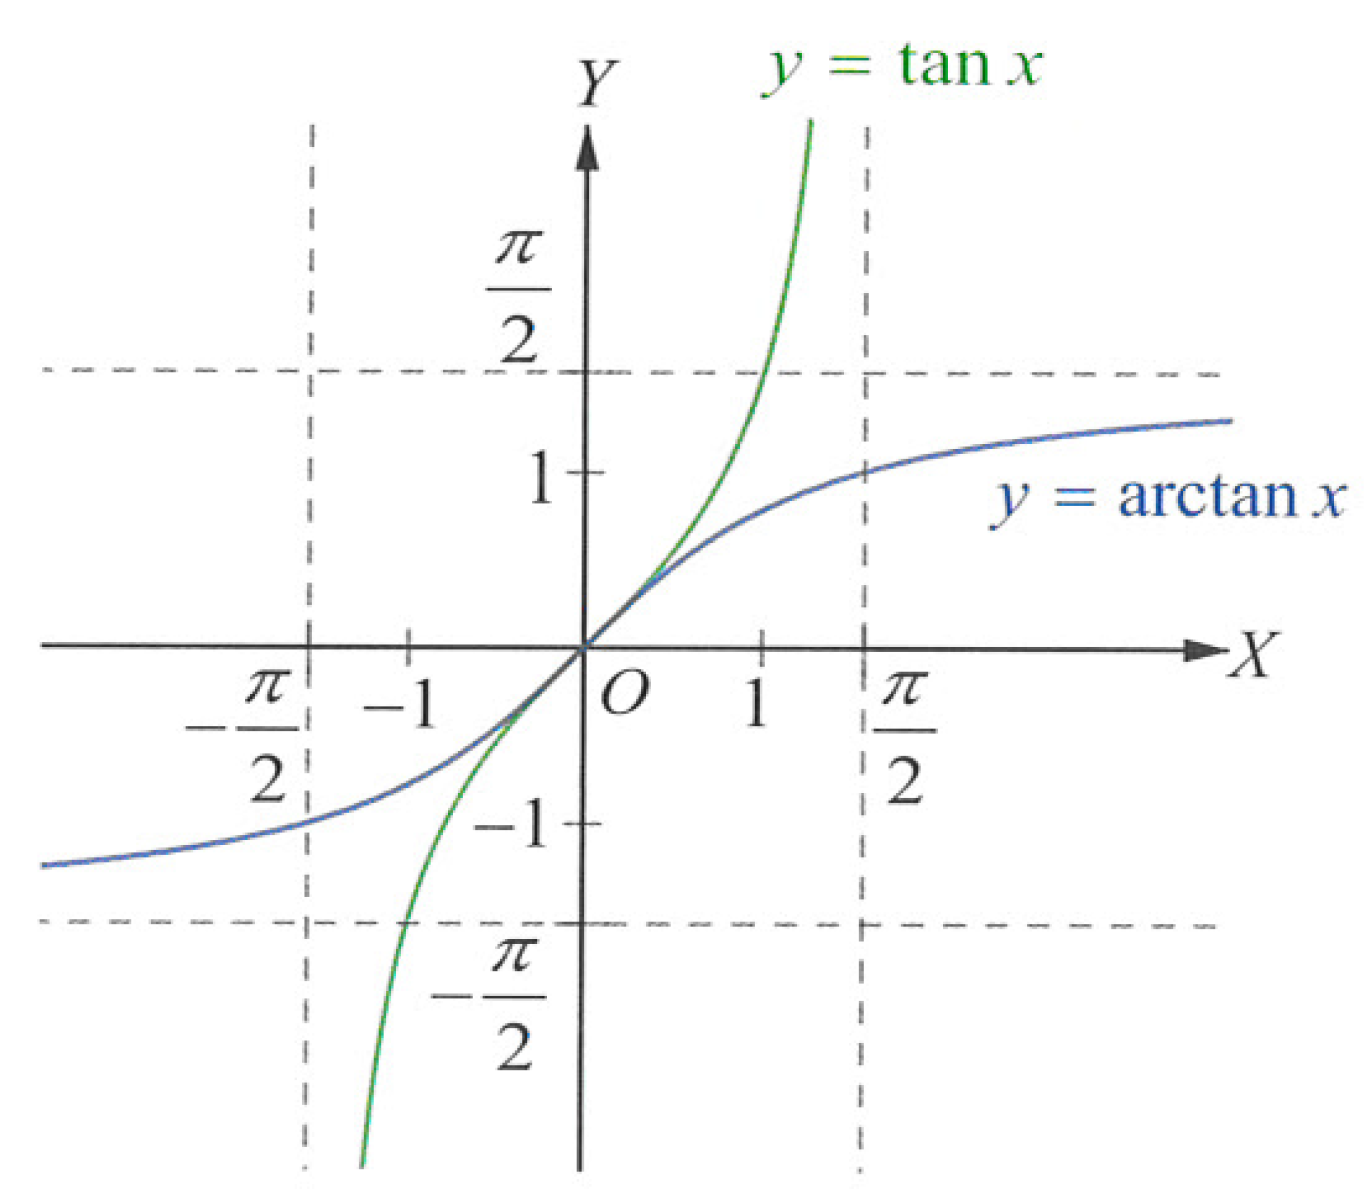
\includegraphics[scale=0.55]{50} 
	\caption{} 
	\label{Figure50} 
\end{figure}

$$
y=\arctan x \quad \text{เมื่อ } -\infty < x < \infty \text{ และ } -\dfrac{\pi}{2} < y < \dfrac{\pi}{2}
$$

\noindent จะเห็นว่า โดเมนของฟังก์ชัน arctangent คือ $\mathbb{R}$ และเรนจ์ของฟังก์ชัน arctangent คือ $\left( -\dfrac{\pi}{2}, \dfrac{\pi}{2} \right)$

\begin{examplebox}
จงหาค่าของ $\arctan 1$
\end{examplebox}
\solution
\newpage

\begin{examplebox}
จงหาค่าของ $\arctan (-\sqrt{3})$
\end{examplebox}
\solution
\vspace{5cm}

สรุปได้ว่า ฟังก์ชันตรีโกณมิติที่กำหนดโดเมนเพื่อให้มีฟังก์ชันผกผัน มีโดเมนและเรนจ์ ดังนี้

\begin{figure}[H] 
	\centering 
	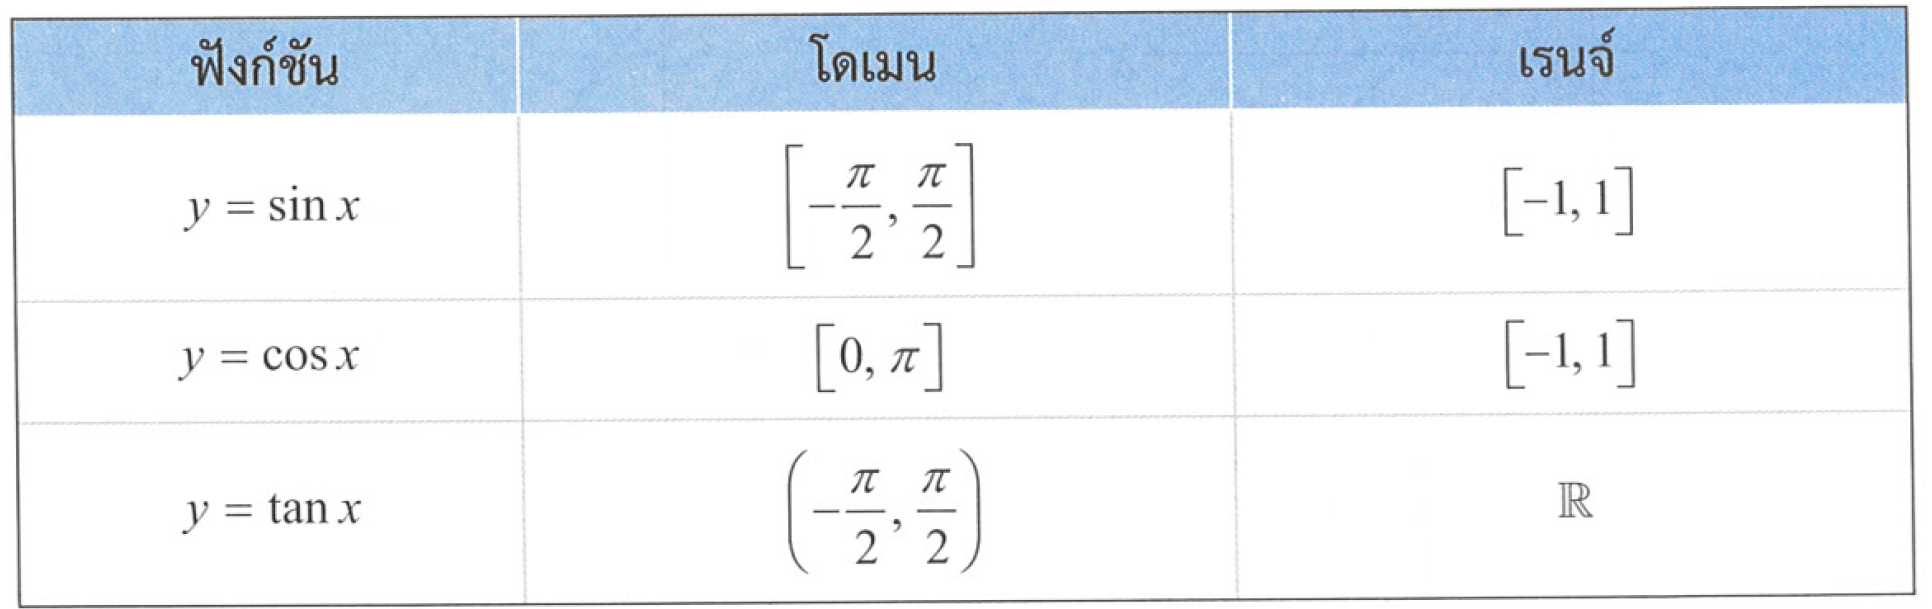
\includegraphics[scale=0.55]{51} 
	\caption{} 
	\label{Figure51} 
\end{figure}

\noindent และฟังก์ชัน $\arcsin$, $\arccos$ และ $\arctan$ มีโดเมนและเรนจ์ ดังนี้

\begin{figure}[H] 
	\centering 
	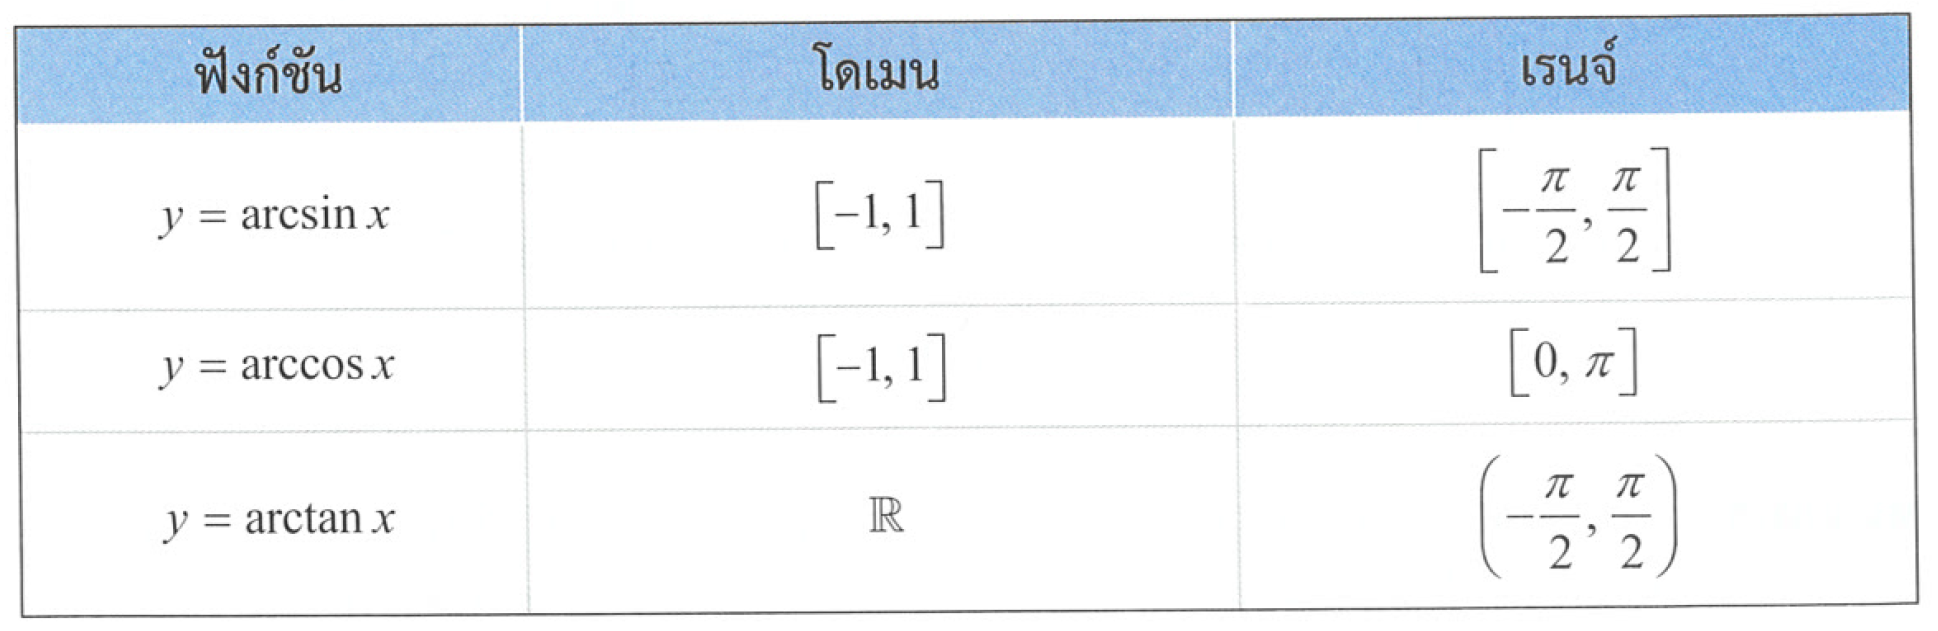
\includegraphics[scale=0.55]{52} 
	\caption{} 
	\label{Figure52} 
\end{figure}
\newpage

กราฟของฟังก์ชัน sine, cosine, tangent, arcsine, arccosine และ arctangent เป็นดังนี้
\begin{figure}[H] 
	\centering 
	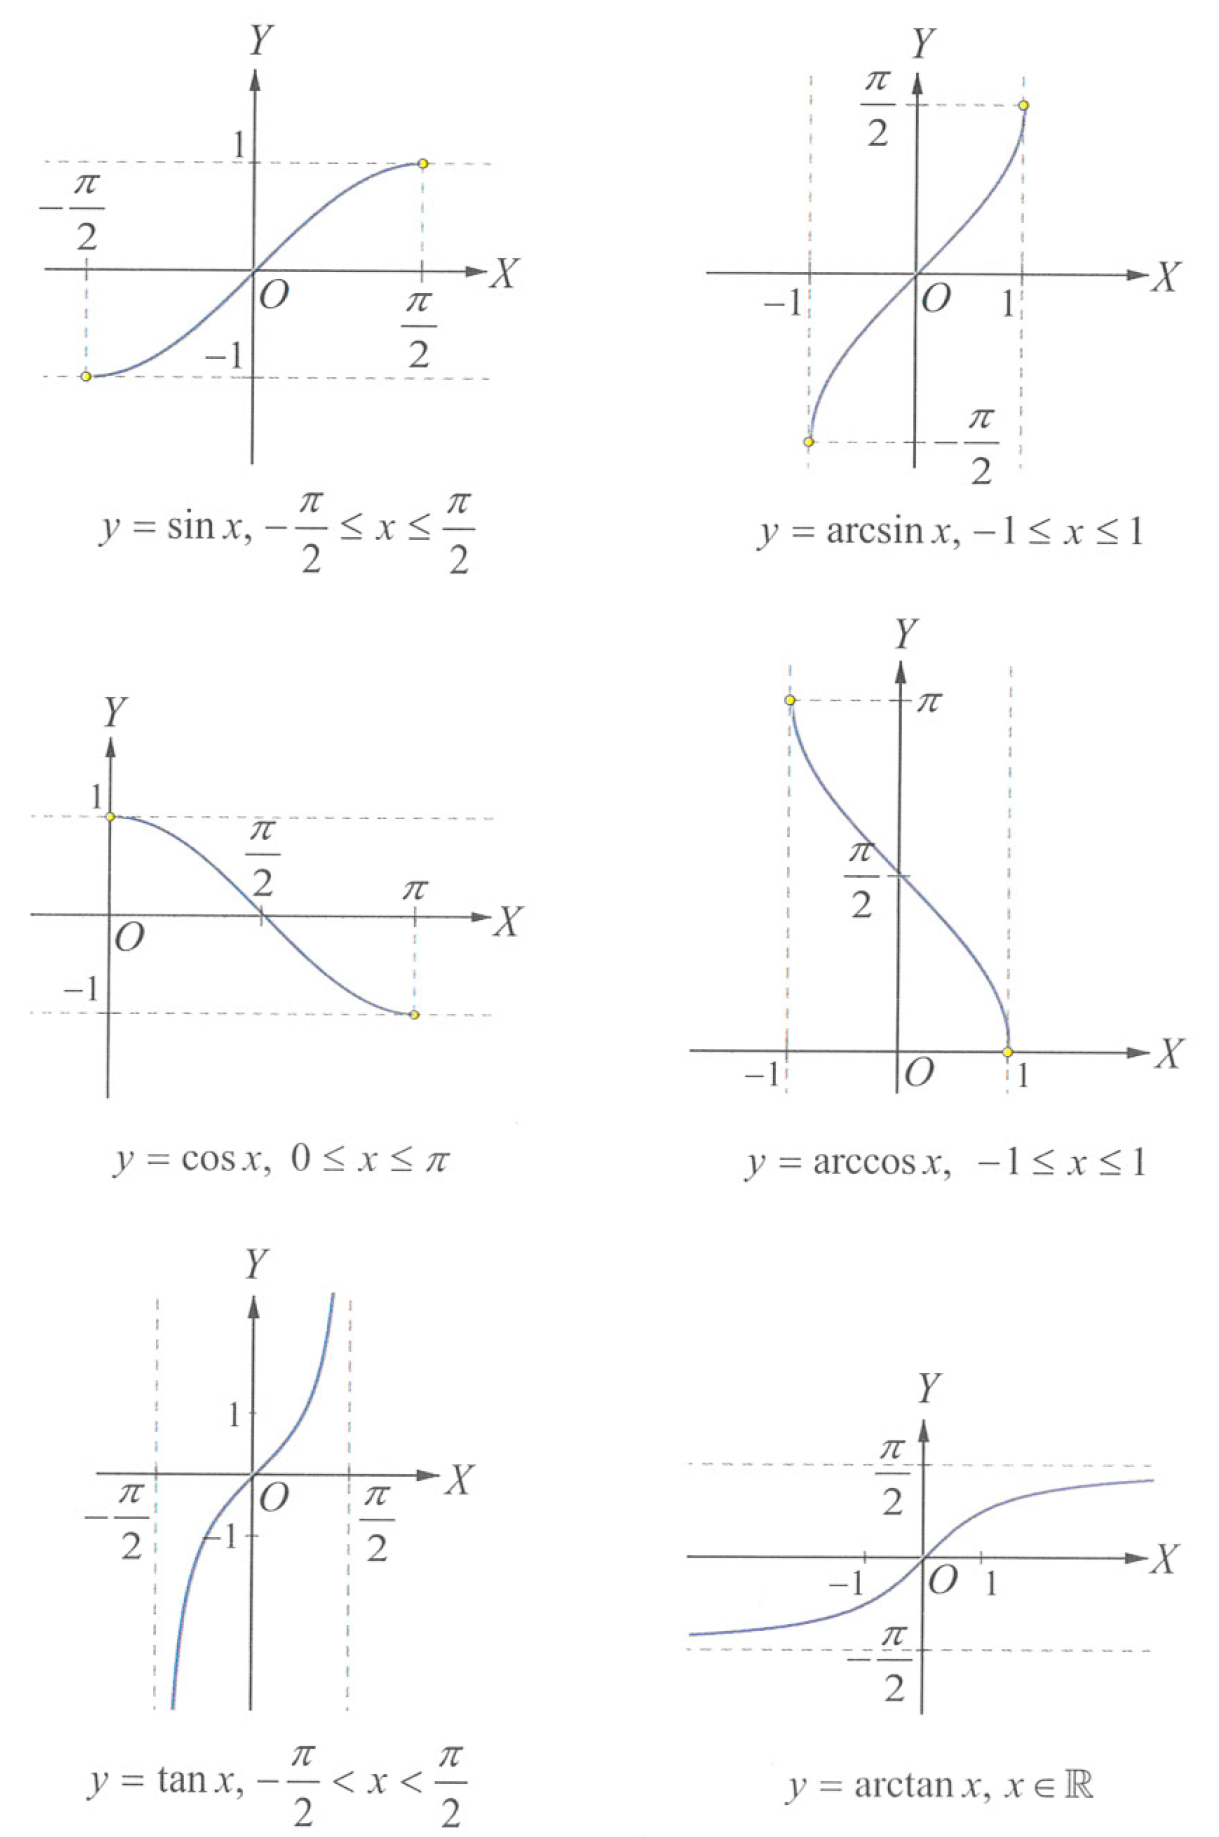
\includegraphics[scale=0.60]{53} 
	\caption{} 
	\label{Figure53} 
\end{figure}
\vspace{0.5em}
\remark หนังสือบางเล่มเขียนแทนฟังก์ชันผกผันของฟังก์ชันไซน์ ฟังก์ชันโคไซน์ และฟังก์ชันแทนเจนต์ ด้วย $y=\sin^{-1} x$, $y=\cos^{-1} x$ และ $y=\tan^{-1} x$ ตามลำดับ

\newpage
\begin{examplebox}
	จงหาค่าของ $\sin \left( \arccos \left( \dfrac{\sqrt{3}}{2} \right) \right)$
\end{examplebox}
\solution
\vspace{5cm}

\begin{examplebox}
	จงหาค่าของ $\cos \left( 2 \arccos \left( \dfrac{1}{3} \right) \right)$
\end{examplebox}
\solution
\newpage

\begin{examplebox}
	จงหาค่าของ $\cos \left( \arcsin \left( -\dfrac{1}{3} \right) \right)$
\end{examplebox}
\solution
\newpage

\begin{examplebox}
	จงแสดงว่า $\sin (\arctan x) = \dfrac{x}{\sqrt{1+x^{2}}}$
\end{examplebox}
\solution ให้ $\arctan x = \theta$ \\
จะได้ $\tan \theta = x$ โดยที่ $\left( -\dfrac{\pi}{2} < \theta < \dfrac{\pi}{2} \right)$ \\
จาก $1 + \tan^{2} \theta = \sec^{2} \theta$ \\
จะได้ $\sec \theta = \sqrt{1 + \tan^{2} \theta}$ หรือ $\sec \theta = -\sqrt{1 + \tan^{2} \theta}$ \\
เนื่องจาก $-\dfrac{\pi}{2} < \theta < \dfrac{\pi}{2}$ จะได้ $\sec \theta > 0$ นั่นคือ $\sec \theta = \sqrt{1 + \tan^{2} \theta}$ \\
ดังนั้น $\sin (\arctan x) = \sin \theta$

$$
\begin{aligned}
	\sin \theta &= \cos \theta \cdot \dfrac{\sin \theta}{\cos \theta} \\
	&= \dfrac{\tan \theta}{\sec \theta} \\
	&= \dfrac{\tan \theta}{\sqrt{1 + \tan^{2} \theta}} \\
	&= \dfrac{x}{\sqrt{1 + x^{2}}}
\end{aligned}
$$
\newpage
\begin{examplebox}
	สะพานข้ามแม่น้ำแห่งหนึ่งมีส่วนตรงกลางที่สามารถเปิดให้เรือผ่านได้ยาว $60$ เมตร โดยแบ่งเป็นสองส่วนเท่ากัน และเปิดขึ้นจากตรงกลาง ถ้าขณะที่เปิดสะพาน ส่วนที่สูงสุดอยู่สูงจากแนวเดิมของสะพาน $18$ เมตร จงหาว่าสะพานเปิดขึ้นไปเป็นมุมเท่าใด
\end{examplebox}
\solution ให้ $\theta$ เป็นมุมที่สะพานเปิดขึ้นไป จากโจทย์ เขียนรูปได้ดังนี้

\begin{figure}[H] 
	\centering 
	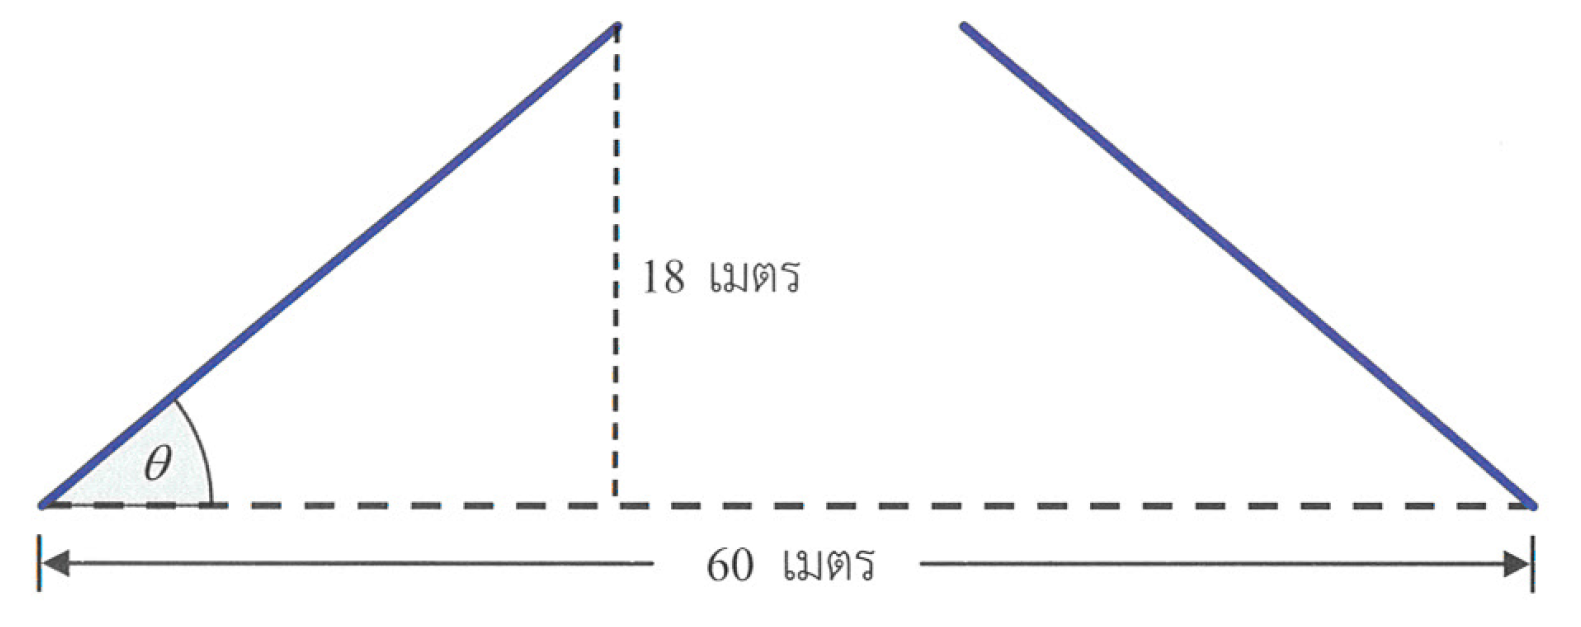
\includegraphics[scale=0.60]{54} 
	\caption{} 
	\label{Figure54} 
\end{figure}
\newpage
\section{เอกลักษณ์และสมการตรีโกณมิติ}
\subsection{เอกลักษณ์}
พิจารณาสมการต่อไปนี้

$$
\begin{aligned}
	\cot \theta &= \dfrac{1}{\tan \theta} \quad \text{เมื่อ } \tan \theta \neq 0 \\
	\sin \theta &= \cos \theta
\end{aligned}
$$

\noindent จะเห็นว่า สมการทั้งสองเป็นสมการที่มีฟังก์ชันตรีโกณมิติปรากฏอยู่ เรียกสมการเช่นนี้ว่า \textbf{สมการตรีโกณมิติ}

สมการ $\cot \theta = \dfrac{1}{\tan \theta}$ จะเป็นจริงสำหรับทุกค่าของ $\theta$ ที่ทำให้หาค่าของฟังก์ชันที่ปรากฏอยู่ในสมการนั้นได้ คือ ค่าของ $\cot \theta$, $\tan \theta$ และ $\dfrac{1}{\tan \theta}$ เรียกสมการที่มีสมบัติเช่นสมการ $\cot \theta = \dfrac{1}{\tan \theta}$ ว่า \textbf{เอกลักษณ์}

ส่วนสมการ $\sin \theta = \cos \theta$ จะเป็นจริงสำหรับบางค่าของ $\theta$ ที่อยู่ในโดเมนของฟังก์ชันทั้งสองเท่านั้น

ในเรื่องฟังก์ชันตรีโกณมิติที่ผ่านมาได้มีการพิสูจน์เอกลักษณ์มาบ้างแล้ว เช่น เอกลักษณ์ต่อไปนี้

$$
\begin{aligned}
	\sin^{2} \theta + \cos^{2} \theta &= 1 \\
	1 + \tan^{2} \theta &= \sec^{2} \theta \\
	1 + \cot^{2} \theta &= \cosec^{2} \theta \\
	\sin (-\theta) &= -\sin \theta \\
	\cos (-\theta) &= \cos \theta \\
	\cos (\alpha + \beta) &= \cos \alpha \cos \beta - \sin \alpha \sin \beta \\
	\tan (\alpha - \beta) &= \dfrac{\tan \alpha - \tan \beta}{1 + \tan \alpha \tan \beta} \\
	\sin 2 \alpha &= 2 \sin \alpha \cos \alpha
\end{aligned}
$$

การพิสูจน์เอกลักษณ์เป็นการแสดงให้เห็นว่าจำนวนทั้งสองข้างของเครื่องหมายเท่ากับของสมการเท่ากันจริง โดยใช้ความรู้เกี่ยวกับฟังก์ชันตรีโกณมิติ การพิสูจน์เอกลักษณ์จึงช่วยให้เห็นความสัมพันธ์ต่าง ๆ ระหว่างฟังก์ชันตรีโกณมิติ และเอกลักษณ์ที่พิสูจน์แล้วสามารถนำไปอ้างอิงในการพิสูจน์เอกลักษณ์อื่น ๆ ได้

\begin{examplebox}
	จงพิสูจน์ว่า $\dfrac{2 \cos^{2} \theta - \sin^{2} \theta + 1}{\cos \theta} = 3 \cos \theta$
\end{examplebox}
\solution พิสูจน์ จากด้านซ้ายของสมการ จะได้
$$
\begin{aligned}
	\dfrac{2 \cos^{2} \theta - \sin^{2} \theta + 1}{\cos \theta} &= \dfrac{2 \cos^{2} \theta - (1 - \cos^{2} \theta) + 1}{\cos \theta} \\
	&= \dfrac{3 \cos^{2} \theta}{\cos \theta} \\
	&= 3 \cos \theta
\end{aligned}
$$

\begin{examplebox}
	จงพิสูจน์ว่า $\dfrac{\cos \theta}{1 - \sin \theta} = \dfrac{1 + \sin \theta}{\cos \theta}$
\end{examplebox}
\solution พิสูจน์ จากด้านซ้ายของสมการ จะได้
$$
\begin{aligned}
	\dfrac{\cos \theta}{1 - \sin \theta} &= \dfrac{\cos \theta}{1 - \sin \theta} \cdot \left( \dfrac{1 + \sin \theta}{1 + \sin \theta} \right) \\
	&= \dfrac{\cos \theta (1 + \sin \theta)}{1 - \sin^{2} \theta} \\
	&= \dfrac{\cos \theta (1 + \sin \theta)}{\cos^{2} \theta} \\
	&= \dfrac{1 + \sin \theta}{\cos \theta}
\end{aligned}
$$

\begin{examplebox}
	จงพิสูจน์ว่า $\dfrac{\sin x}{1 + \cos x} = \tan\left(\dfrac{x}{2}\right)$
\end{examplebox}
\solution พิสูจน์ โดยใช้สูตรมุมครึ่งเท่า (Half-angle identity) จะได้
$$
\begin{aligned}
	\dfrac{\sin x}{1 + \cos x} &= \dfrac{\sin 2\left(\dfrac{x}{2}\right)}{1 + \cos 2\left(\dfrac{x}{2}\right)} \\
	&= \dfrac{2 \sin \dfrac{x}{2} \cos \dfrac{x}{2}}{1 + 2 \cos^{2} \dfrac{x}{2} - 1} \\
	&= \dfrac{2 \sin \dfrac{x}{2} \cos \dfrac{x}{2}}{2 \cos^{2} \dfrac{x}{2}} \\
	&= \dfrac{\sin \dfrac{x}{2}}{\cos \dfrac{x}{2}} \\
	&= \tan \dfrac{x}{2}
\end{aligned}
$$

\newpage
\begin{examplebox}
	จงพิสูจน์ว่า $\dfrac{\cos 3x - \cos 5x}{\sin 3x + \sin 5x} = \tan x$
\end{examplebox}
\solution พิสูจน์ โดยใช้สูตรแปลงผลบวกผลต่างเป็นผลคูณจะได้
$$
\begin{aligned}
	\dfrac{\cos 3x - \cos 5x}{\sin 3x + \sin 5x} &= \dfrac{-2 \sin \left(\dfrac{3x + 5x}{2}\right) \sin \left(\dfrac{3x - 5x}{2}\right)}{2 \sin \left(\dfrac{3x + 5x}{2}\right) \cos \left(\dfrac{3x - 5x}{2}\right)} \\
	&= \dfrac{-2 \sin 4x \sin (-x)}{2 \sin 4x \cos (-x)} \\
	&= \dfrac{-(-\sin x)}{\cos x} \\
	&= \tan x
\end{aligned}
$$

\begin{examplebox}
	กำหนด $A + B + C = \pi$ จงพิสูจน์ว่า $\tan A + \tan B + \tan C = \tan A \tan B \tan C$
\end{examplebox}
\solution พิสูจน์ จาก $A + B + C = \pi$ จะได้ $A + B = \pi - C$
$$
\begin{aligned}
	\tan (A + B) &= \tan (\pi - C) \\
	\dfrac{\tan A + \tan B}{1 - \tan A \tan B} &= -\tan C \\
	\tan A + \tan B &= -\tan C (1 - \tan A \tan B) \\
	\tan A + \tan B &= -\tan C + \tan A \tan B \tan C
\end{aligned}
$$
ดังนั้น $\tan A + \tan B + \tan C = \tan A \tan B \tan C$

\newpage
\subsection{สมการตรีโกณมิติ}
การแก้สมการตรีโกณมิติทำได้ในทำนองเดียวกันกับการแก้สมการทั่วไป เช่น สมการเอกซ์โพเนนเชียลหรือสมการลอการิทึม โดยอาศัยความรู้เกี่ยวกับฟังก์ชันตรีโกณมิติ เพื่อหาคำตอบของสมการ

เนื่องจากฟังก์ชันตรีโกณมิติไม่เป็นฟังก์ชัน $1-1$ ค่าของฟังก์ชันตรีโกณมิติของจำนวนจริงหรือมุมใด ๆ อาจจะซ้ำกันได้ ดังนั้น ในการหาคำตอบของสมการ ถ้าโจทย์ไม่ได้กำหนดให้คำตอบอยู่ในช่วงใดช่วงหนึ่งแล้ว คำตอบควรจะอยู่ในรูปของค่าทั่วไป

\begin{examplebox}
	จงหาเซตคำตอบของสมการ $\cos x = \dfrac{1}{2}$ เมื่อ $\left( 0 < x < \dfrac{\pi}{2} \right)$
\end{examplebox}
\solution พิสูจน์ เนื่องจากค่าของ $x$ ในช่วง $\left( 0, \dfrac{\pi}{2} \right)$ ที่ทำให้ $\cos x = \dfrac{1}{2}$ คือ $\dfrac{\pi}{3}$ เพียงค่าเดียว 
\newline
ดังนั้น เซตคำตอบ คือ $\left\{ \dfrac{\pi}{3} \right\}$

\begin{examplebox}
	จงแก้สมการ $\sin \theta = \dfrac{1}{2}$
\end{examplebox}
\solution ค่าของ $\theta$ ในช่วง $\left[ 0, 2 \pi \right]$ ที่ทำให้ $\sin \theta = \dfrac{1}{2}$ คือ $\dfrac{\pi}{6}$ และ $\dfrac{5 \pi}{6}$
\newline
เนื่องจาก $\sin \left( 2 n \pi + \dfrac{\pi}{6} \right) = \sin \dfrac{\pi}{6} = \dfrac{1}{2}$ เมื่อ $n \in \mathbb{Z}$
\newline
และ $\sin \left( 2 n \pi + \dfrac{5 \pi}{6} \right) = \sin \dfrac{\pi}{6} = \dfrac{1}{2}$ เมื่อ $n \in \mathbb{Z}$
\newline
ดังนั้น ค่าทั่วไปของ $\theta$ ที่ทำให้สมการเป็นจริง คือ $2 n \pi + \dfrac{\pi}{6}$ และ $2 n \pi + \dfrac{5 \pi}{6}$ เมื่อ $n$ เป็นจำนวนเต็ม

\newpage
\begin{examplebox}
	จงแก้สมการ $\tan x = 1$
\end{examplebox}
\solution วิธีทำ จาก $\tan x = 1$ จะได้ 
$$
\begin{aligned}
	\dfrac{\sin x}{\cos x} &= 1 \\
	\sin x &= \cos x
\end{aligned}
$$

\begin{figure}[H] 
	\centering 
	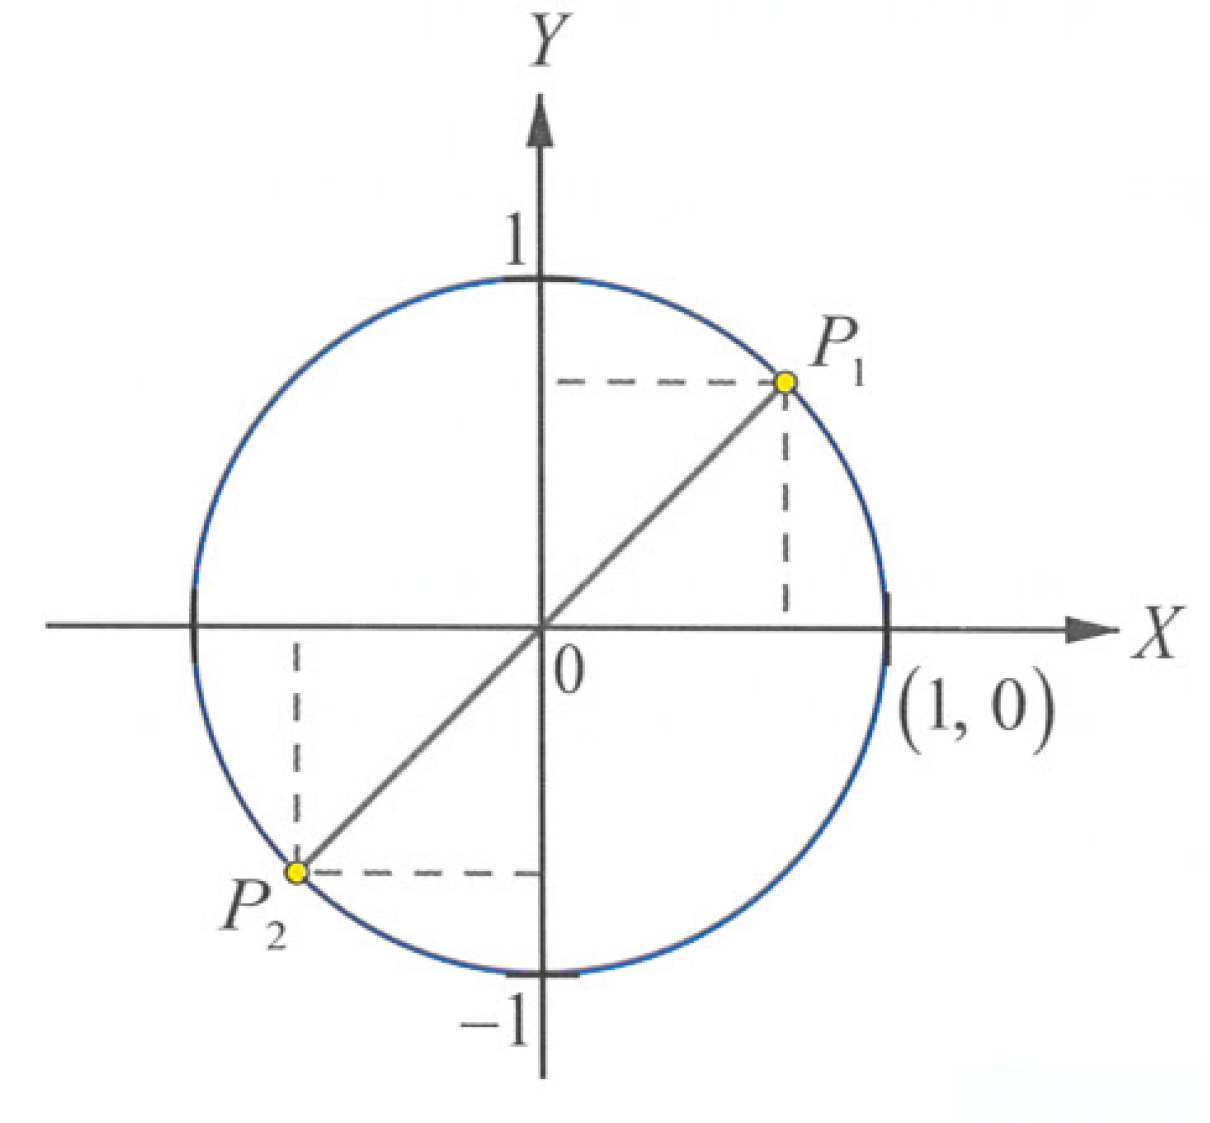
\includegraphics[scale=0.60]{55} 
	\caption{} 
	\label{Figure55} 
\end{figure}

\noindent จากรูป ถ้า $\sin x = \cos x$ แสดงว่าจุด $P_{1}$ และ $P_{2}$ มีพิกัดแรกและพิกัดที่สองเท่ากัน นั่นคือ $x = \dfrac{\pi}{4}$ และ $x = \dfrac{5 \pi}{4}$
\newline
ดังนั้น ค่าทั่วไปของ $x$ ที่ทำให้สมการเป็นจริง คือ $2 n \pi + \dfrac{\pi}{4}$ และ $2 n \pi + \dfrac{5 \pi}{4}$ เมื่อ $n$ เป็นจำนวนเต็ม

\vspace{0.5em}
\remark จากตัวอย่างข้างต้น เนื่องจาก $2 n \pi + \dfrac{5 \pi}{4} = (2 n + 1) \pi + \dfrac{\pi}{4}$ เมื่อ $n \in \mathbb{Z}$ 
\newline
ดังนั้น เซตคำตอบคือ $\left\{ x \;\middle|\; x = n \pi + \dfrac{\pi}{4}, \, n \in \mathbb{Z} \right\}$

\newpage
\begin{examplebox}
	จงแก้สมการ $2 \sin^{2} \theta + 3 \cos \theta - 3 = 0$ เมื่อ $0^{\circ} \leq \theta \leq 360^{\circ}$
\end{examplebox}
\solution จากโจทย์จัดรูปสมการให้อยู่ในรูปฟังก์ชันโคไซน์ จะได้
$$
\begin{aligned}
	2 \sin^{2} \theta + 3 \cos \theta - 3 &= 0 \\
	2(1 - \cos^{2} \theta) + 3 \cos \theta - 3 &= 0 \\
	2 - 2 \cos^{2} \theta + 3 \cos \theta - 3 &= 0 \\
	2 \cos^{2} \theta - 3 \cos \theta + 1 &= 0 \\
	(2 \cos \theta - 1)(\cos \theta - 1) &= 0
\end{aligned}
$$
นั่นคือ $\cos \theta = \dfrac{1}{2}$ หรือ $\cos \theta = 1$
\newline
ค่าของ $\theta$ ในช่วง $\left[ 0^{\circ}, 360^{\circ} \right]$ ที่ทำให้ $\cos \theta = \dfrac{1}{2}$ คือ $60^{\circ}$ และ $300^{\circ}$
\newline
และค่าของ $\theta$ ในช่วง $\left[ 0^{\circ}, 360^{\circ} \right]$ ที่ทำให้ $\cos \theta = 1$ คือ $0^{\circ}$ และ $360^{\circ}$
\newline
ดังนั้น ค่าของ $\theta$ ในช่วง $\left[ 0^{\circ}, 360^{\circ} \right]$ ที่ทำให้สมการเป็นจริง คือ $0^{\circ}, 60^{\circ}, 300^{\circ}$ และ $360^{\circ}$

\begin{examplebox}
	จงแก้สมการ $\sin \theta + \cos \theta = 1$
\end{examplebox}
\solution ยกกำลังสองทั้งสองข้างของสมการ จะได้
$$
\begin{aligned}
	\sin \theta + \cos \theta &= 1 \\
	(\sin \theta + \cos \theta)^{2} &= 1 \\
	\sin^{2} \theta + 2 \sin \theta \cos \theta + \cos^{2} \theta &= 1 \\
	2 \sin \theta \cos \theta + 1 &= 1 \\
	2 \sin \theta \cos \theta &= 0 \\
	\sin 2 \theta &= 0
\end{aligned}
$$
จะได้ $2 \theta = 0$ หรือ $2 \theta = \pi$ หรือ $2 \theta = 2 \pi$ หรือ $2 \theta = 3 \pi$
\newline
นั่นคือ $\theta = 0$ หรือ $\theta = \dfrac{\pi}{2}$ หรือ $\theta = \pi$ หรือ $\theta = \dfrac{3 \pi}{2}$ เมื่อ $\theta \in [0, 2 \pi)$

\vspace{0.5em}
\noindent \textbf{ตรวจคำตอบ:} แทนค่า $\theta$ ในสมการ $\sin \theta + \cos \theta = 1$
\begin{itemize}
	\item แทน $\theta = 0$ จะได้ $\sin 0 + \cos 0 = 1 \implies 1 = 1$ (เป็นจริง)
	\item แทน $\theta = \dfrac{\pi}{2}$ จะได้ $\sin \dfrac{\pi}{2} + \cos \dfrac{\pi}{2} = 1 \implies 1 = 1$ (เป็นจริง)
	\item แทน $\theta = \pi$ จะได้ $\sin \pi + \cos \pi = 1 \implies -1 = 1$ (เป็นเท็จ)
	\item แทน $\theta = \dfrac{3 \pi}{2}$ จะได้ $\sin \dfrac{3 \pi}{2} + \cos \dfrac{3 \pi}{2} = 1 \implies -1 = 1$ (เป็นเท็จ)
\end{itemize}
จะได้ คำตอบของสมการ $\sin \theta + \cos \theta = 1$ ในช่วง $[0, 2 \pi)$ คือ $0$ และ $\dfrac{\pi}{2}$
\newline
ดังนั้น คำตอบทั่วไปของสมการ คือ $2 n \pi$ และ $2 n \pi + \dfrac{\pi}{2}$ เมื่อ $n$ เป็นจำนวนเต็ม

\newpage
\section{กฎของโคไซน์และกฎของไซน์}
เนื่องจากฟังก์ชันตรีโกณมิติเป็นฟังก์ชันของจำนวนจริงหรือมุม สมบัติของฟังก์ชันตรีโกณมิติอาจนำมาใช้ในการหาความยาวของด้านและขนาดของมุมของรูปหลายเหลี่ยมได้ โดยเฉพาะรูปสามเหลี่ยม ซึ่งจะกล่าวถึงความสัมพันธ์ระหว่างด้านและมุมของรูปสามเหลี่ยมและฟังก์ชันตรีโกณมิติดังนี้

\begin{theorembox}[กฎของโคไซน์]
	ให้รูปสามเหลี่ยม $ABC$ มีด้านตรงข้ามมุม $A, \, B$ และ $C$ ยาว $a, \, b$ และ $c$ หน่วย ตามลำดับ จะได้
	$$
	\begin{aligned}
		a^{2} &= b^{2} + c^{2} - 2bc \cos A \\
		b^{2} &= c^{2} + a^{2} - 2ca \cos B \\
		c^{2} &= a^{2} + b^{2} - 2ab \cos C
	\end{aligned}
	$$
\end{theorembox}

พิสูจน์ ให้มุม $A$ ของรูปสามเหลี่ยม $ABC$ ที่กำหนดให้อยู่ในตำแหน่งมาตรฐาน

\begin{figure}[H] 
	\centering 
	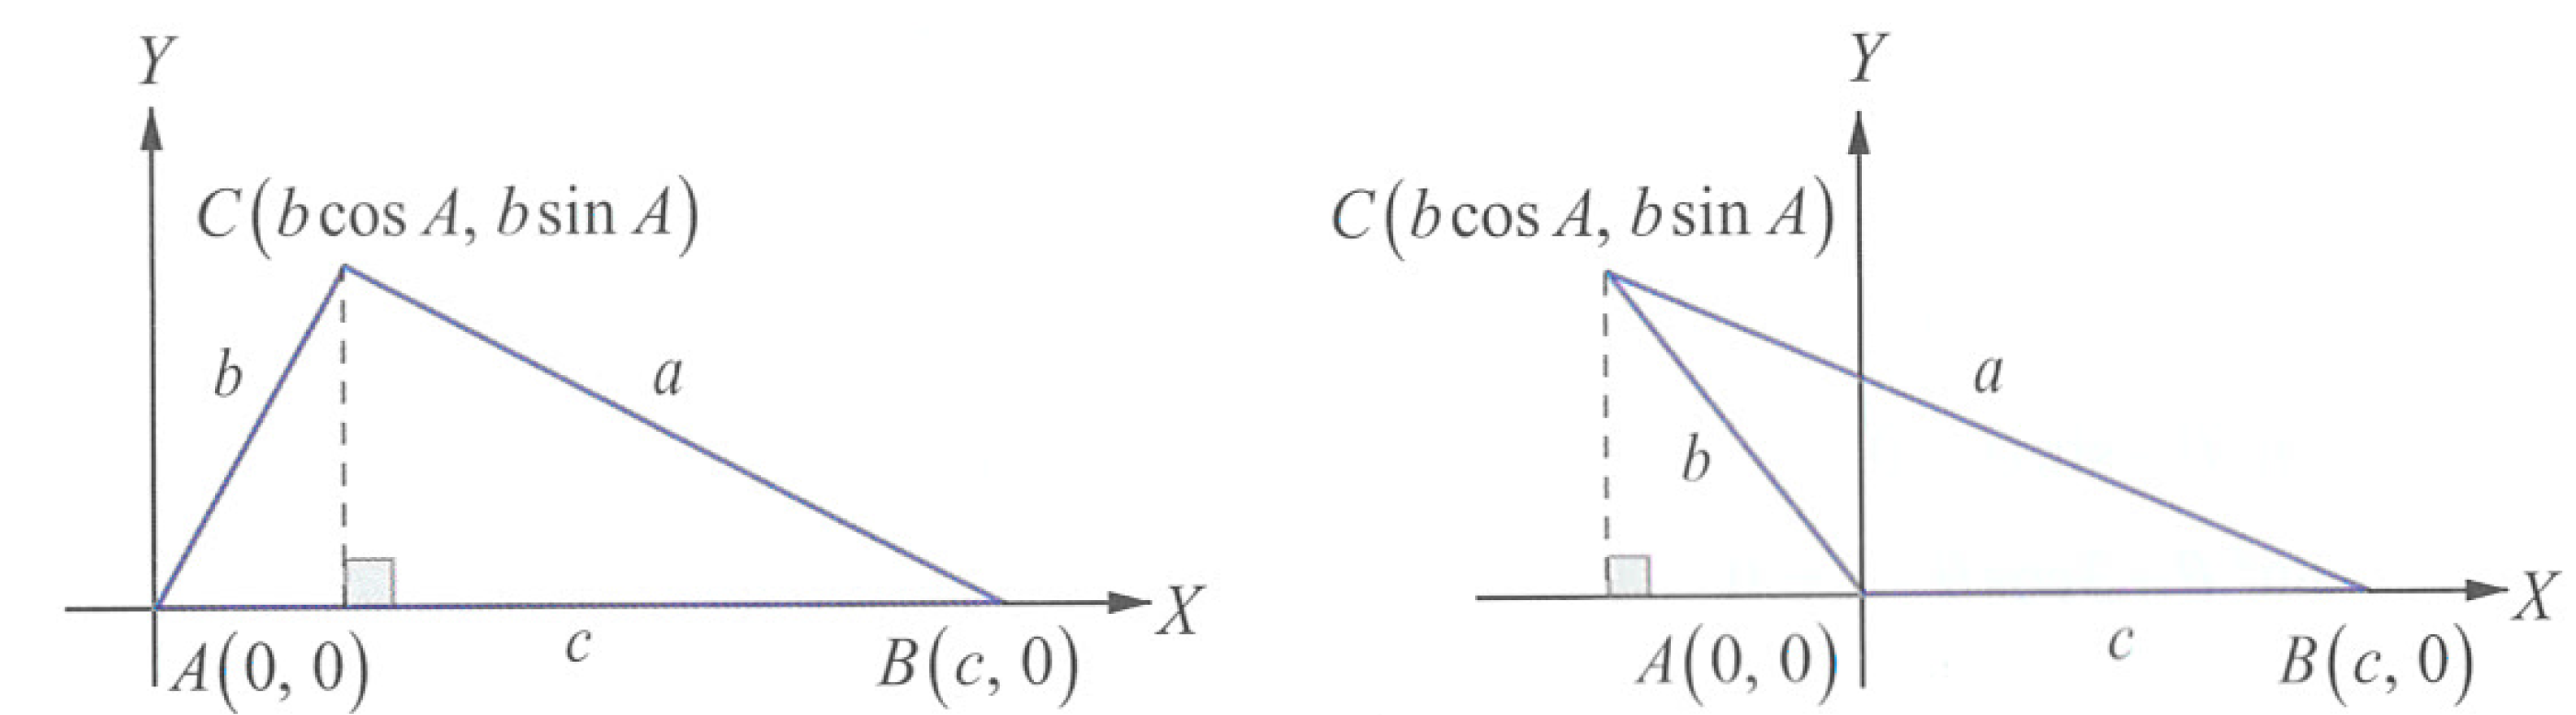
\includegraphics[scale=0.4]{56} 
	\caption{} 
	\label{Figure56} 
\end{figure}

\noindent จากรูป จุด $A$ มีพิกัด $(0,0)$ และจุด $B$ มีพิกัด $(c, 0)$ 
\newline
จะได้ จุด $C$ มีพิกัด $(b \cos A, \, b \sin A)$ และ $a = \sqrt{(b \cos A - c)^{2} + (b \sin A - 0)^{2}}$
$$
\begin{aligned}
	a^{2} &= (b \cos A - c)^{2} + b^{2} \sin^{2} A \\
	&= b^{2} \cos^{2} A - 2bc \cos A + c^{2} + b^{2} \sin^{2} A \\
	&= b^{2}(\cos^{2} A + \sin^{2} A) + c^{2} - 2bc \cos A \\
	&= b^{2} + c^{2} - 2bc \cos A
\end{aligned}
$$
ดังนั้น $a^{2} = b^{2} + c^{2} - 2bc \cos A$
\newline
สำหรับ $b^{2} = c^{2} + a^{2} - 2ca \cos B$ และ $c^{2} = a^{2} + b^{2} - 2ab \cos C$ สามารถพิสูจน์ได้ในทำนองเดียวกัน

\vspace{0.5em}
กฎของโคไซน์นี้ใช้หาความยาวของด้านหรือขนาดของมุมของรูปสามเหลี่ยม เมื่อกำหนดความยาวของด้านบางด้านและขนาดของมุมบางมุม ดังตัวอย่างต่อไปนี้
\begin{examplebox}
ให้รูปสามเหลี่ยม $A B C$ มีด้านตรงข้ามมุม $A, B$ และ $C$ ยาว $a, b$ และ $c$ หน่วย ตามลำดับ ถ้า $a=12, b=7, C=40^{\circ}$ และ $\cos 40^{\circ} \approx 0.766$ จงหาค่าของ $c$
\end{examplebox}
\solution
\newpage
\begin{theorembox}[กฎของไซน์]
	ให้รูปสามเหลี่ยม $ABC$ มีด้านตรงข้ามมุม $A, \, B$ และ $C$ ยาว $a, \, b$ และ $c$ หน่วย ตามลำดับ จะได้
	$$
	\dfrac{\sin A}{a} = \dfrac{\sin B}{b} = \dfrac{\sin C}{c}
	$$
\end{theorembox}

\noindent พิสูจน์ ให้มุม $A$ ของรูปสามเหลี่ยม $ABC$ ที่กำหนดให้อยู่ในตำแหน่งมาตรฐาน

\begin{figure}[H] 
	\centering 
	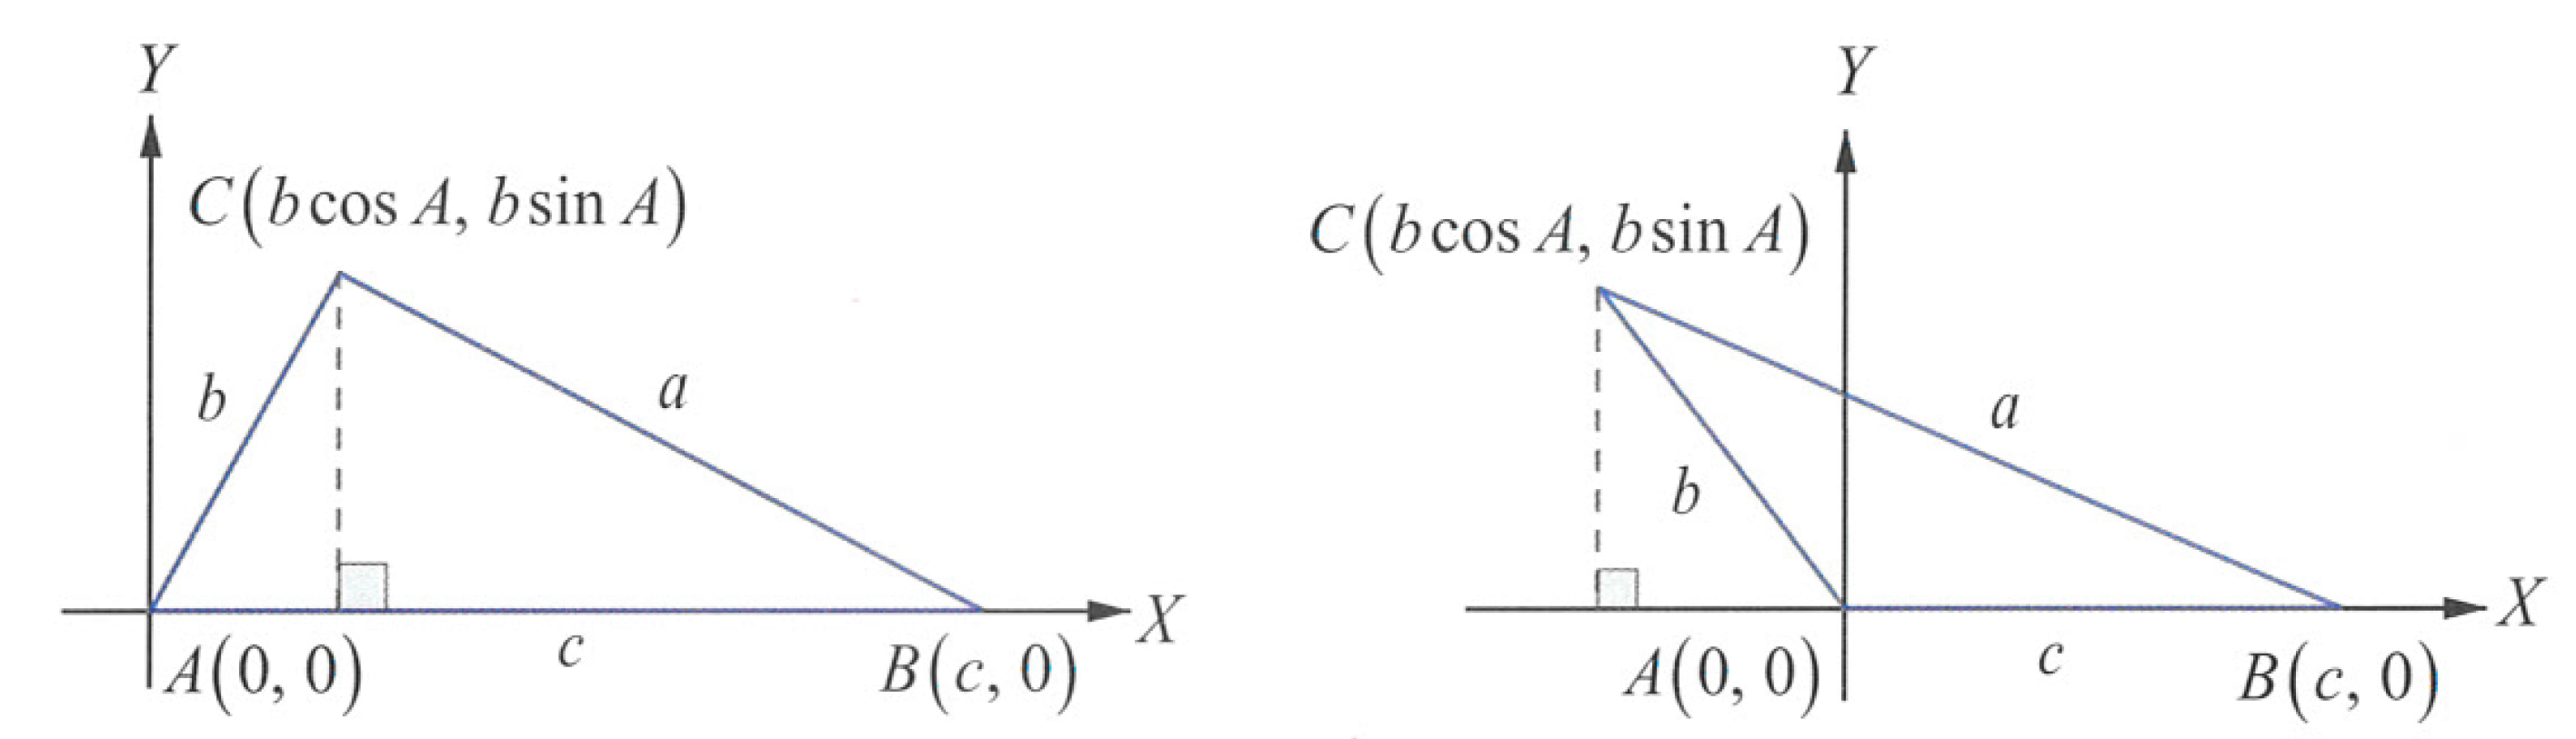
\includegraphics[scale=0.38]{57} 
	\caption{} 
	\label{Figure57} 
\end{figure}

\noindent จากรูป จุด $A$ มีพิกัด $(0,0)$ และจุด $B$ มีพิกัด $(c, 0)$
\newline
จะได้ จุด $C$ มีพิกัด $(b \cos A, \, b \sin A)$
\newline
จากสูตร พื้นที่ของรูปสามเหลี่ยม $ABC = \dfrac{1}{2} \times \text{ความสูง} \times \text{ความยาวของฐาน}$
$$
\begin{aligned}
	\text{พื้นที่ของรูปสามเหลี่ยม } ABC &= \dfrac{1}{2}(b \sin A)(c) \\
	&= \dfrac{1}{2}bc \sin A
\end{aligned}
$$

ในทำนองเดียวกัน ถ้าให้มุม $B$ และมุม $C$ อยู่ในตำแหน่งมาตรฐาน แล้วจะสามารถพิสูจน์ได้ว่า พื้นที่ของรูปสามเหลี่ยม $ABC$ เท่ากับ $\dfrac{1}{2}ca \sin B$ และ $\dfrac{1}{2}ab \sin C$ ตามลำดับ
\newline
นั่นคือ $\dfrac{1}{2}bc \sin A = \dfrac{1}{2}ca \sin B = \dfrac{1}{2}ab \sin C$
\newline
เนื่องจาก $a, \, b$ และ $c$ เป็นจำนวนจริงบวก นำ $\dfrac{2}{abc}$ คูณตลอดสมการ จะได้
$$
\left( \dfrac{1}{2}bc \sin A \right) \cdot \left( \dfrac{2}{abc} \right) = \left( \dfrac{1}{2}ca \sin B \right) \cdot \left( \dfrac{2}{abc} \right) = \left( \dfrac{1}{2}ab \sin C \right) \cdot \left( \dfrac{2}{abc} \right)
$$
ดังนั้น
$$
\dfrac{\sin A}{a} = \dfrac{\sin B}{b} = \dfrac{\sin C}{c}
$$

\newpage
กฎของไซน์นี้ใช้หาความยาวของด้านหรือขนาดของมุมของรูปสามเหลี่ยม ดังในตัวอย่างต่อไปนี้
\begin{examplebox}
	ให้รูปสามเหลี่ยม $ABC$ มีด้านตรงข้ามมุม $A, \, B$ และ $C$ ยาว $a, \, b$ และ $c$ หน่วย ตามลำดับ ถ้า $a = 10, \, B = 42^{\circ}, \, C = 51^{\circ}, \, \sin 42^{\circ} \approx 0.6691$ และ $\sin 87^{\circ} \approx 0.9986$ จงหาค่าของ $b$
\end{examplebox}
\solution
\newpage

\begin{examplebox}
	ให้รูปสามเหลี่ยม $ABC$ มีด้านตรงข้ามมุม $A, \, B$ และ $C$ ยาว $a, \, b$ และ $c$ หน่วย ตามลำดับ ถ้า $A = 30^{\circ}, \, a = 2.5$ และ $b = 3.41$ จงหาขนาดของมุม $B$
\end{examplebox}
\solution
\newpage

\begin{examplebox}
	ให้รูปสามเหลี่ยม $ABC$ มีด้านตรงข้ามมุม $A, \, B$ และ $C$ ยาว $a, \, b$ และ $c$ หน่วย ตามลำดับ ถ้า $A = 30^{\circ}, \, a = 32$ และ $b = 24$ จงหาขนาดของมุม $B$
\end{examplebox}
\solution
\newpage

\section{การหาระยะทางและความสูง}
ในการแก้ปัญหาเกี่ยวกับการหาระยะทางและความสูง ซึ่งบางครั้งใช้เครื่องมือวัดโดยตรงไม่ได้ เช่น การวัดความสูงของภูเขา การหาความกว้างของแม่น้ำ สามารถทำได้โดยอาศัยความรู้เรื่องฟังก์ชันตรีโกณมิติ ซึ่งจะมีขนาดของมุมเข้ามาเกี่ยวข้องรวมทั้ง \textbf{มุมก้ม (angle of depression)} และ \textbf{มุมเงย (angle of elevation)}

มุมก้มและมุมเงยเป็นมุมที่เกิดจากแนวเส้นระดับสายตา และแนวเส้นจากตาไปยังวัตถุ ถ้าวัตถุอยู่ต่ำกว่าแนวเส้นระดับสายตา มุมที่ได้เรียกว่า \textbf{มุมก้ม} แต่ถ้าวัตถุอยู่สูงกว่าแนวเส้นระดับสายตา มุมที่ได้เรียกว่า \textbf{มุมเงย} ดังรูป โดยขนาดของมุมก้มและมุมเงยจะเป็นจำนวนจริงบวกเสมอ

\begin{figure}[H] 
	\centering 
	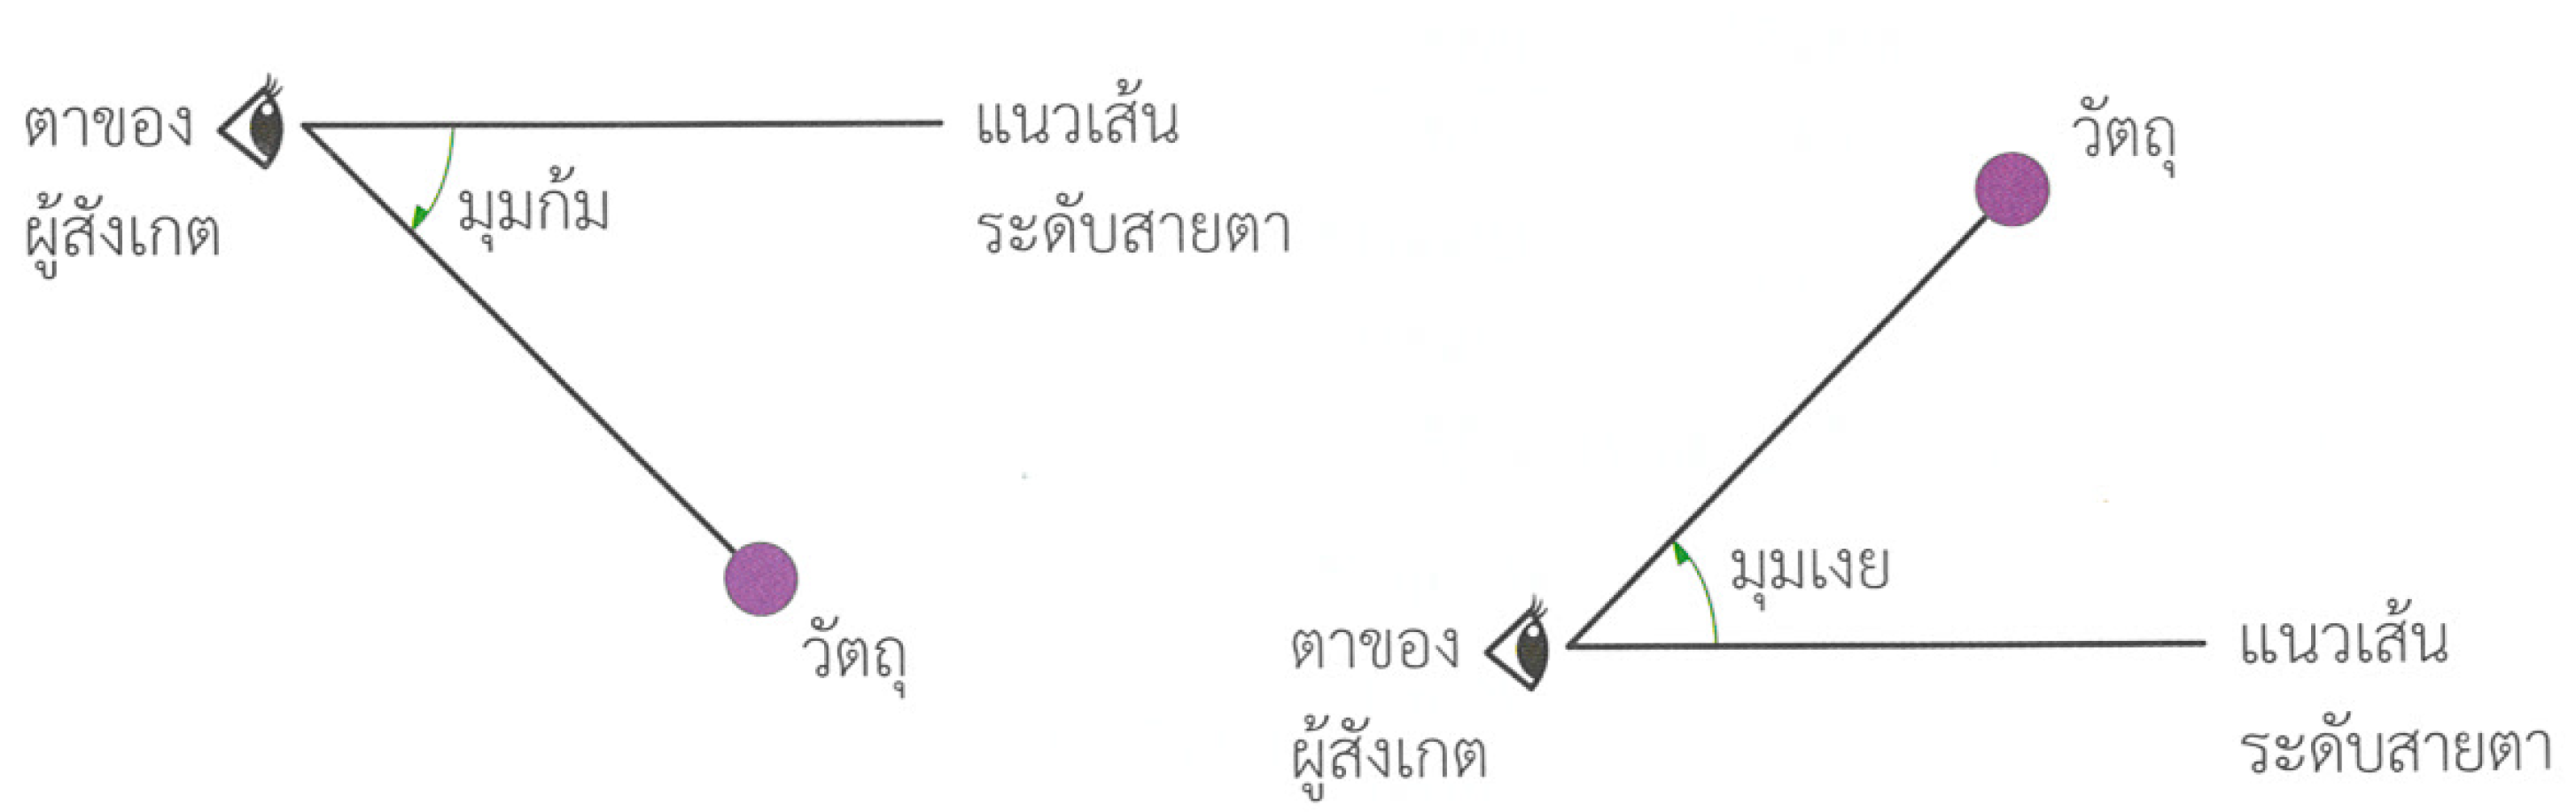
\includegraphics[scale=0.38]{58} 
	\caption{} 
	\label{Figure58} 
\end{figure}

\newpage
\begin{examplebox}
	เนตรยืนอยู่บนสนามแห่งหนึ่งมองเห็นยอดเสาธงเป็นมุมเงย $15^{\circ}$ แต่เมื่อเดินตรงเข้าไปหาเสาธงอีก $60$ เมตร เขามองเห็นยอดเสาธงเป็นมุมเงย $75^{\circ}$ ถ้าเนตรสูง $150$ เซนติเมตร แล้วจงหาความสูงของเสาธง
\end{examplebox}
\solution 

\begin{figure}[H] 
	\centering 
	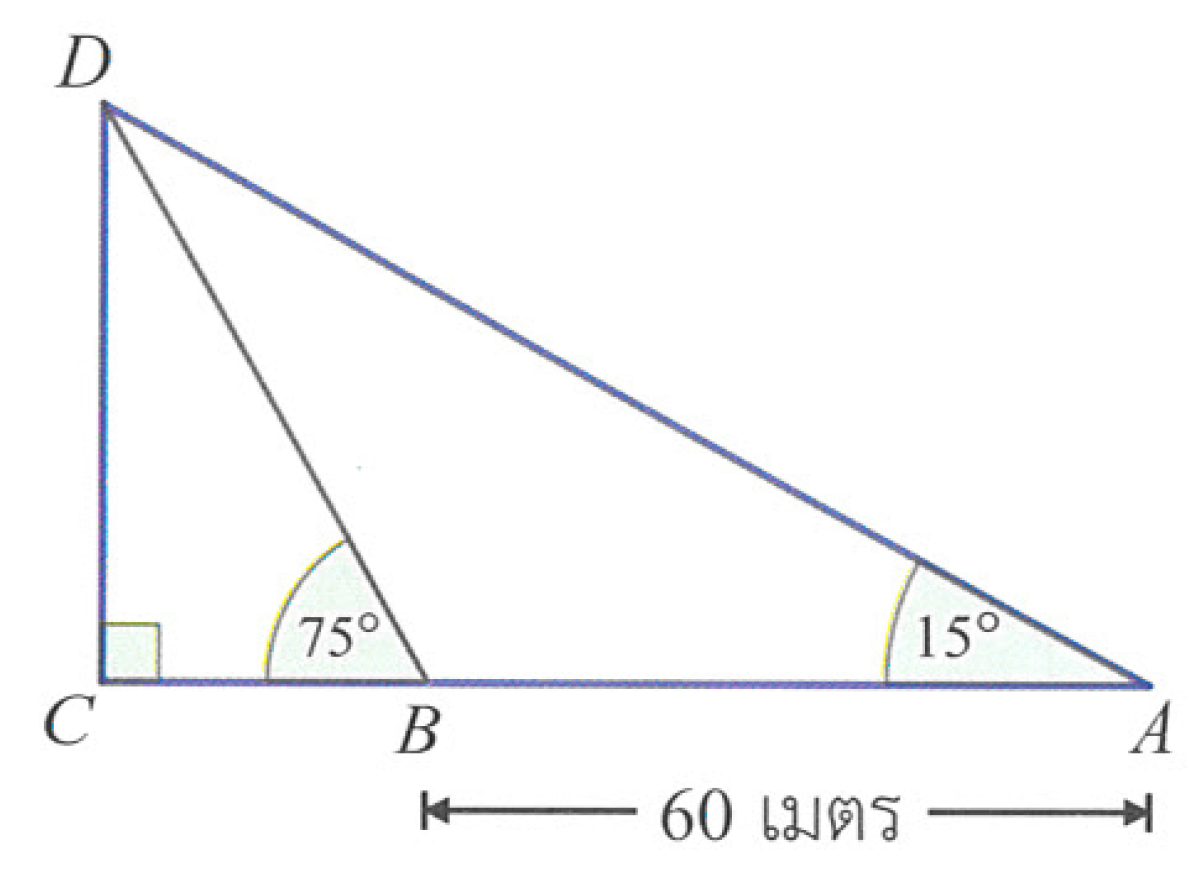
\includegraphics[scale=0.4]{59} 
	\caption{} 
	\label{Figure59} 
\end{figure}

\noindent ให้ $A$ เป็นจุดที่เนตรยืนมองยอดเสาธงในครั้งแรก 
\newline
$B$ เป็นจุดที่เนตรยืนมองยอดเสาธงในครั้งหลัง 
\newline
และ $CD$ เป็นความสูงของเสาธงส่วนที่เหนือระดับสายตา 
\newline
จะได้ ระยะ $AB$ เท่ากับ $60$ เมตร
\newpage
\begin{examplebox}
จากหน้าผาซึ่งสูง $200$ เมตร จากระดับน้ำทะเลปานกลาง ผู้สังเกตการณ์คนหนึ่งมองเห็นเรือสองลำทอดสมออยู่ในทะเลเป็นมุมก้ม $40^{\circ}$ และ $60^{\circ}$ จากเส้นระดับสายตาเส้นเดียวกัน จงหาว่าเรือทั้งสองลำนั้นอยู่ห่างกันเท่าใด
\end{examplebox}
\solution 

\begin{figure}[H] 
	\centering 
	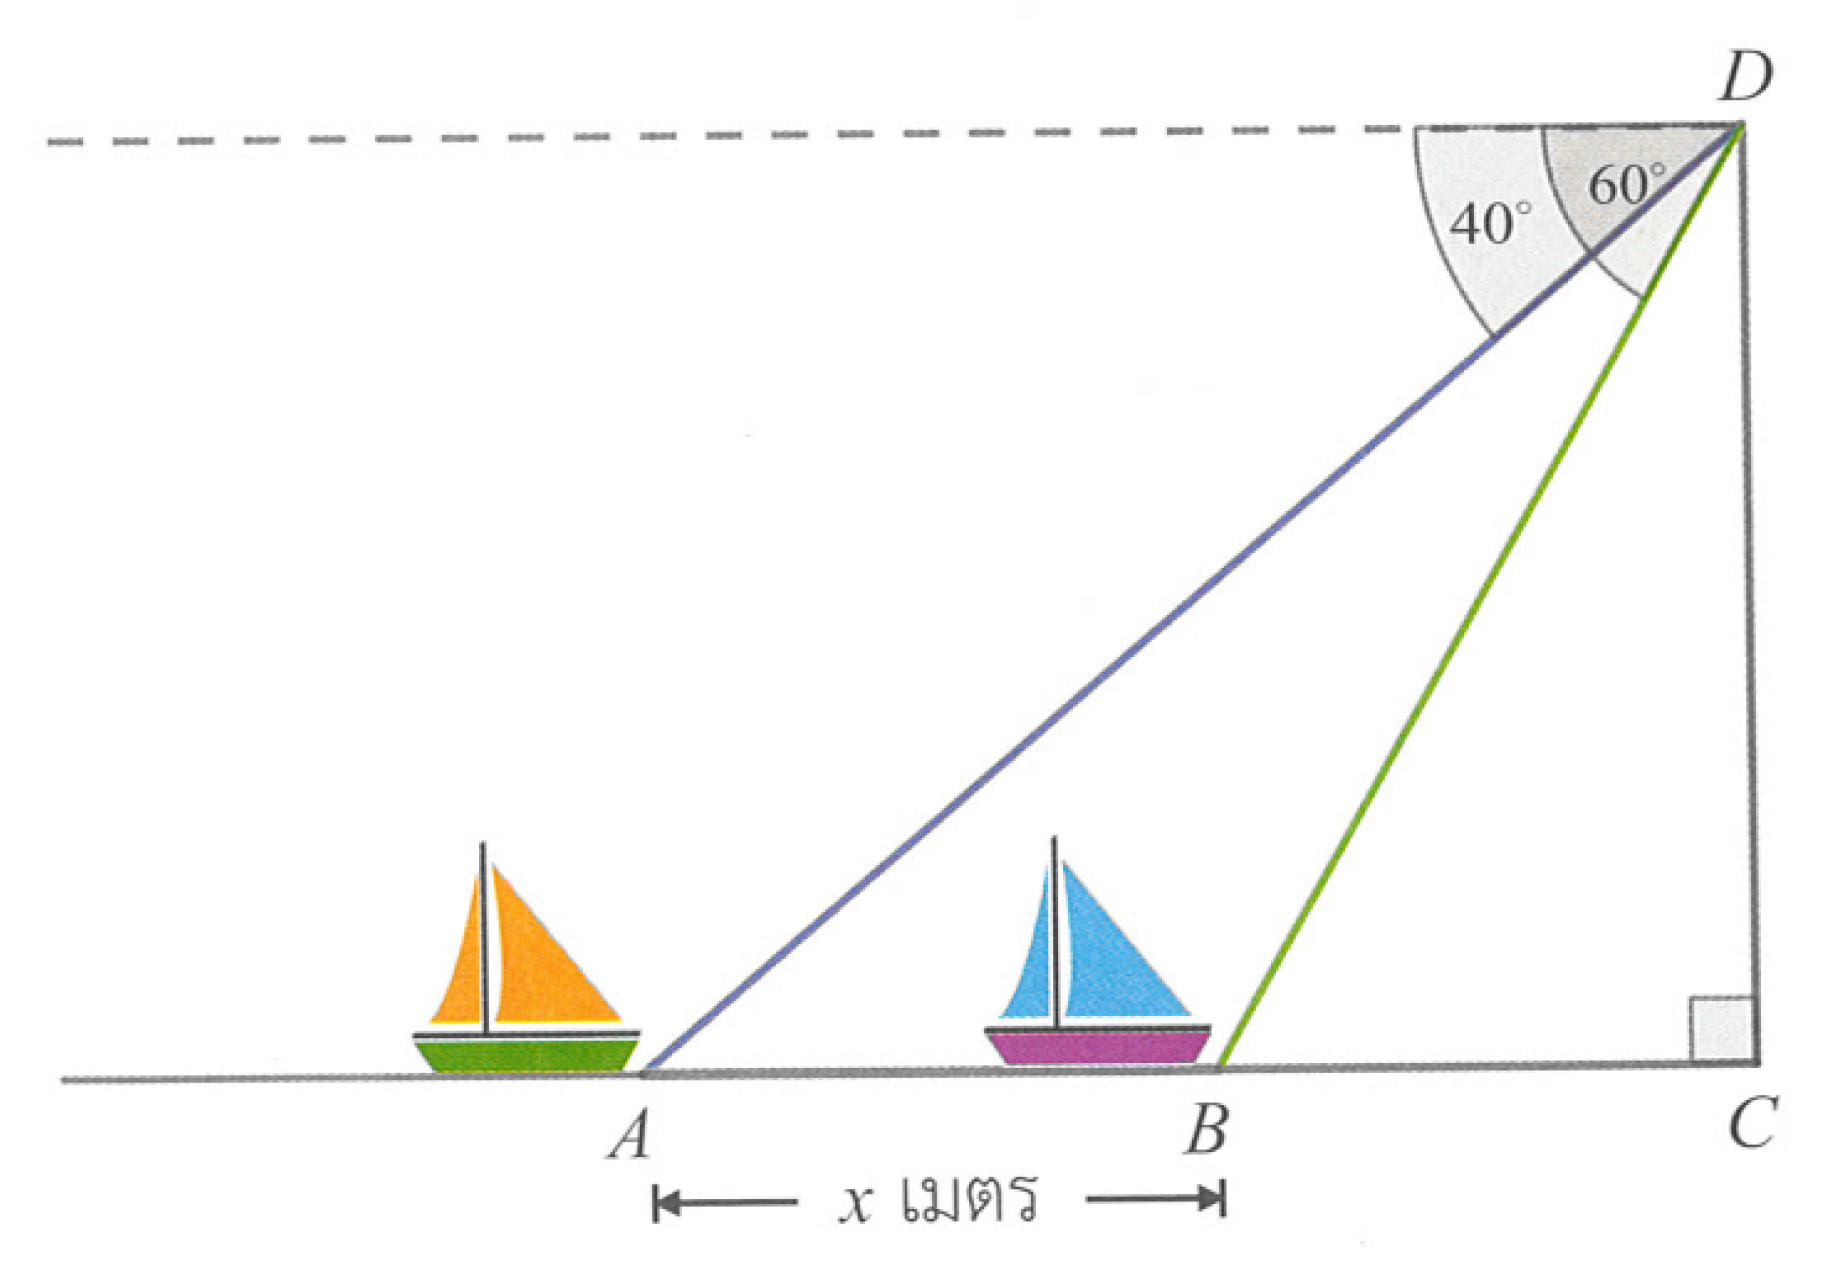
\includegraphics[scale=0.4]{60} 
	\caption{} 
	\label{Figure60} 
\end{figure}

\noindent ให้ $A$ และ $B$ เป็นตำแหน่งของเรือสองลำ โดยให้เรือทั้งสองห่างกัน $x$ เมตร และ $CD$ เป็นความสูงของหน้าผา
\newpage
\begin{examplebox}
	จากรูปที่กำหนดให้ จงหาความสูงของภูเขาตามแนว $SC$ ถ้าวัดระยะ $AB$ ในแนวราบบนพื้นดินได้ $a$ หน่วย และวัดมุม $SAC$ มุม $SBA$ และมุม $SAB$ ได้เป็น $\alpha, \, \beta$ และ $\gamma$ ตามลำดับ
\end{examplebox}
\solution 

\begin{figure}[H] 
	\centering 
	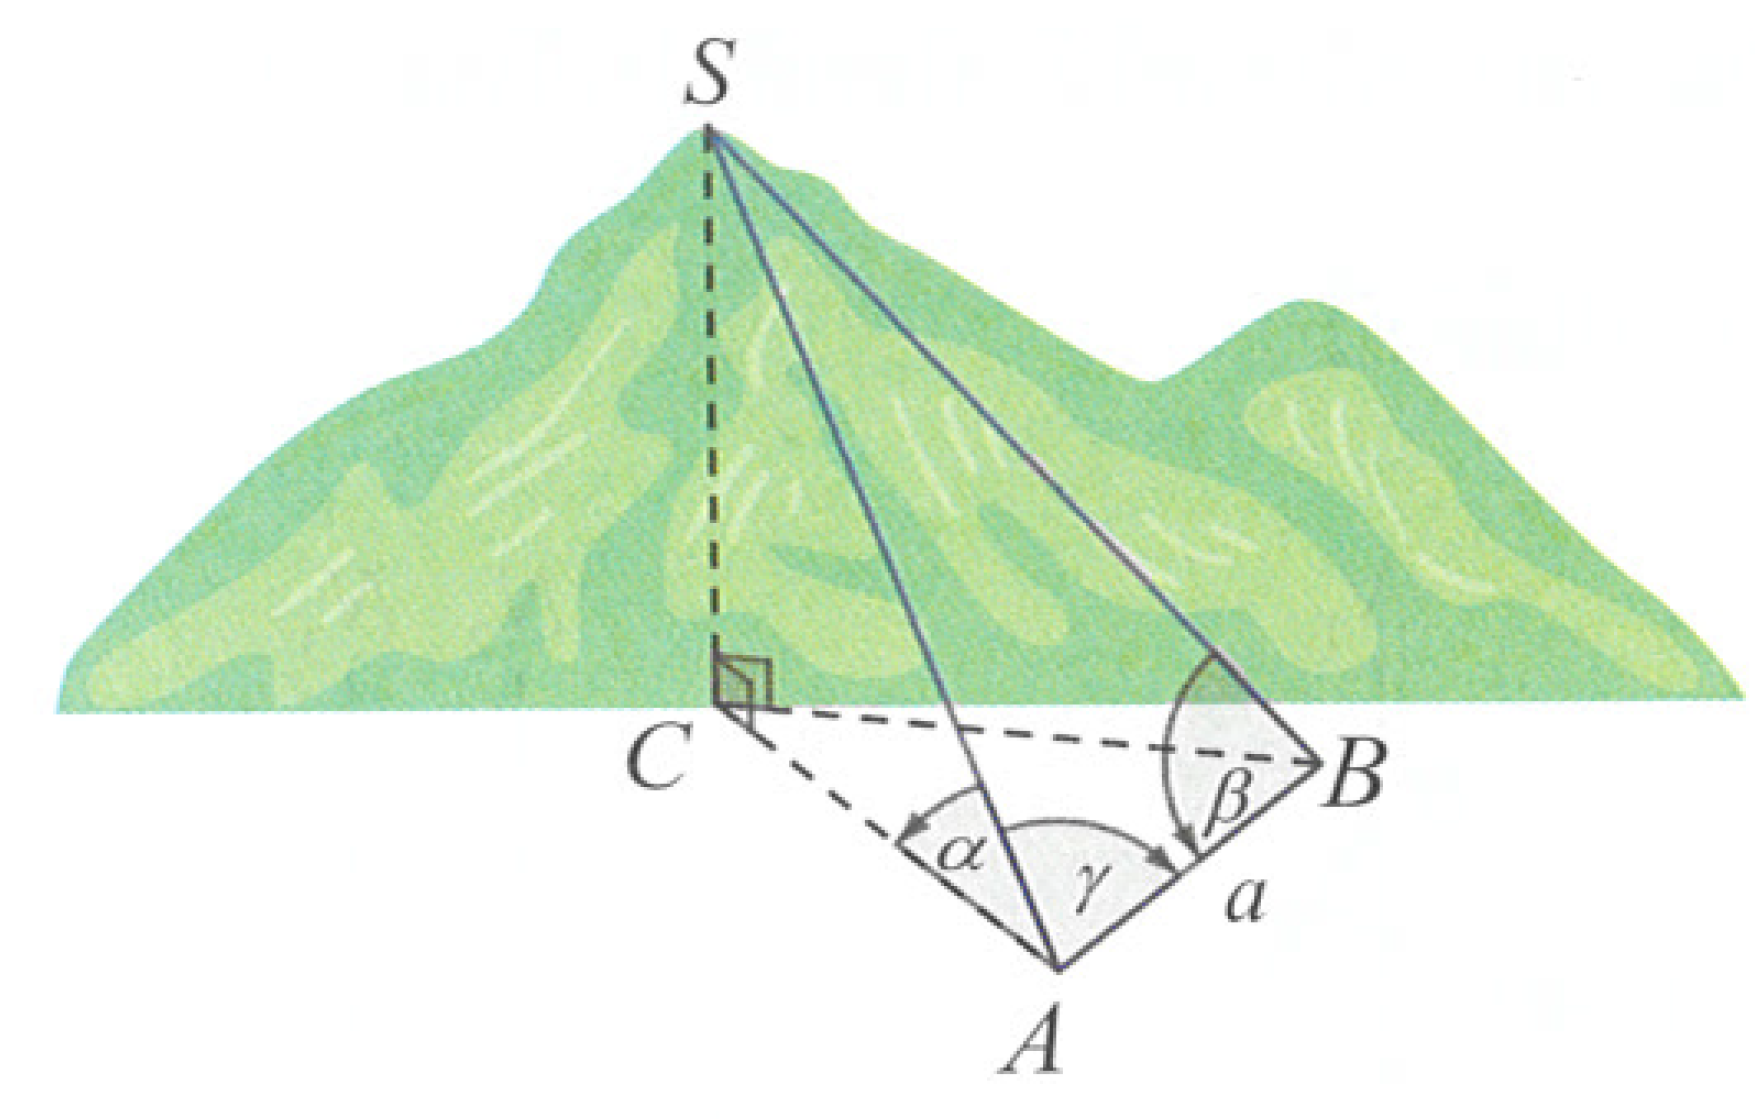
\includegraphics[scale=0.4]{61} 
	\caption{} 
	\label{Figure61} 
\end{figure}


\newpage
\begin{examplebox}
	จากจุด $A$ นักบินบินไปยังจุด $B$ ในแนวเฉียงไปทางทิศตะวันตก โดยทำมุม $38^{\circ} 20^{\prime}$ กับทิศเหนือ เป็นระยะทาง $125$ ไมล์ และบินไปยังจุด $C$ เป็นระยะทาง $125$ ไมล์ ในแนวเฉียงไปทางทิศตะวันออก โดยทำมุม $51^{\circ} 40^{\prime}$ กับทิศใต้ จงหาว่านักบินจะต้องบินจากจุด $C$ ไปในแนวเฉียงไปทางทิศตะวันตก เป็นระยะทางเท่าใด โดยบินทำมุมเท่าใดกับทิศใต้ เพื่อกลับไปยังจุด $A$
\end{examplebox}
\solution 

\begin{figure}[H] 
	\centering 
	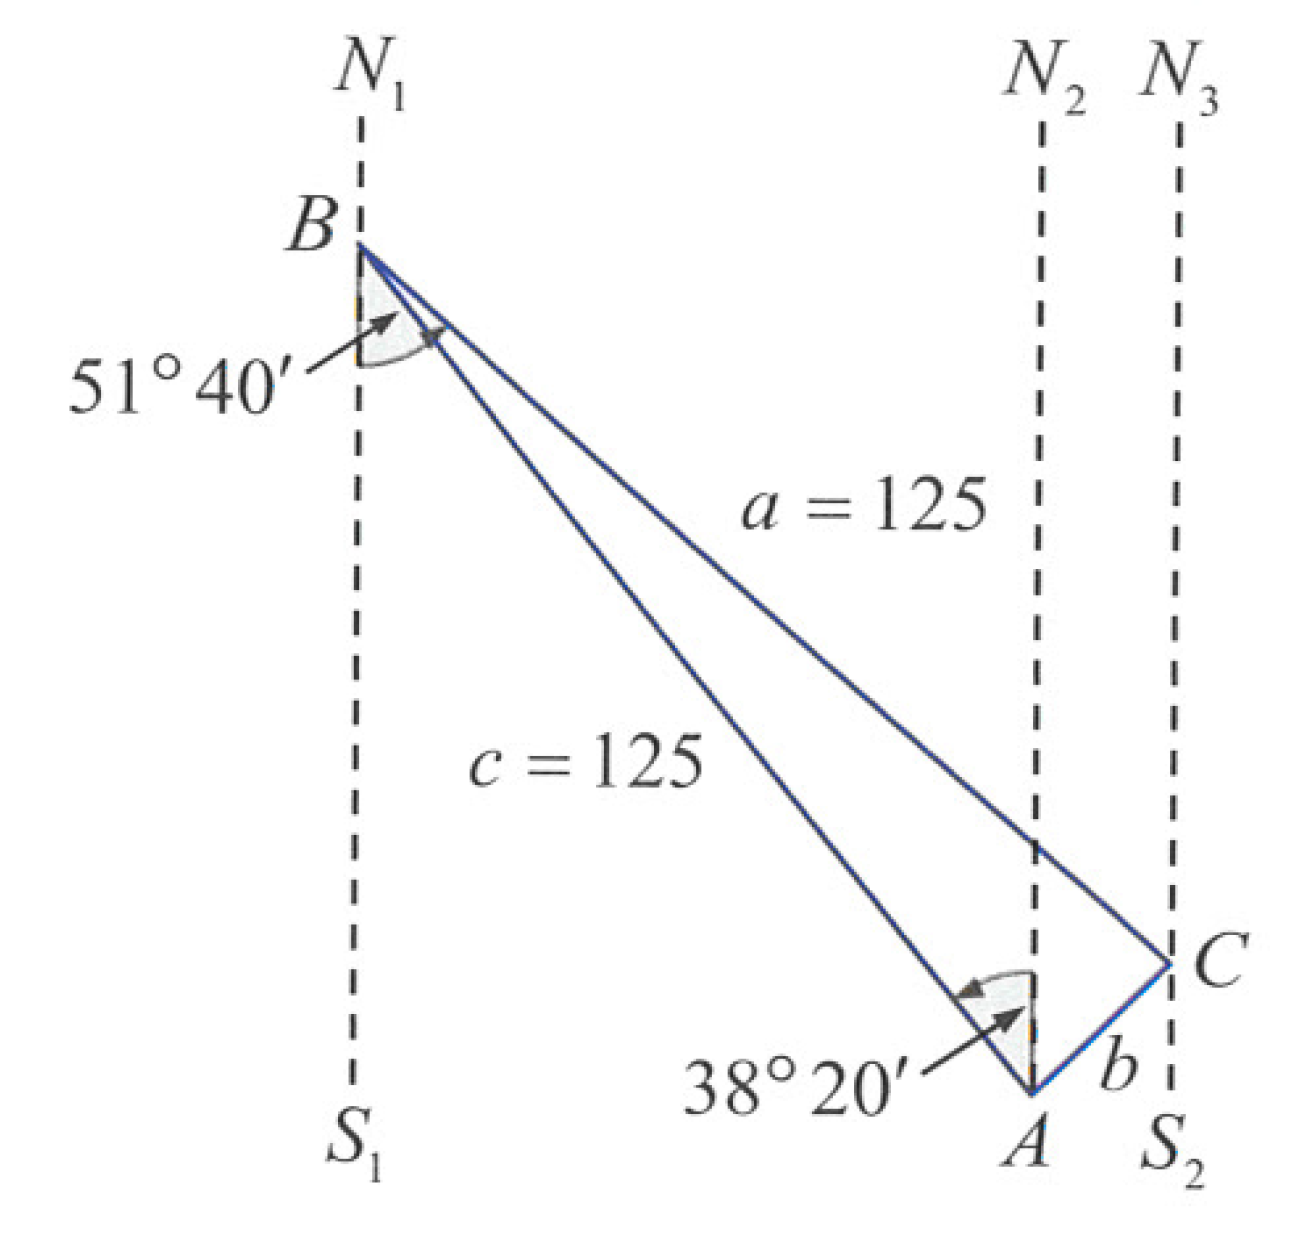
\includegraphics[scale=0.4]{62} 
	\caption{} 
	\label{Figure62} 
\end{figure}